\documentclass{ieeeaccess}
\usepackage{cite}
\usepackage{amsmath,amssymb,amsfonts}
\usepackage{algorithmic}
\usepackage{graphicx}
\usepackage{subfigure}
\usepackage{url}
\usepackage{textcomp}
\usepackage{comment}
\usepackage{epsfig}
\usepackage{verbatim}
\usepackage{cite}
\usepackage{psfrag}
\usepackage{alltt}
\usepackage{indentfirst}
\usepackage{color}
\usepackage{xcolor}
\usepackage{mathrsfs}
\usepackage{amsmath}
\usepackage{scalefnt}
\usepackage{colortbl}
\usepackage{float}
\usepackage{multirow}
\usepackage{flushend}
%\usepackage[table,xcdraw]{xcolor}
\newcolumntype{M}[1]{>{\centering\arraybackslash}m{#1}}

\begin{document}
\history{Date of publication xxxx 00, 0000, date of current version xxxx 00, 0000.}
\doi{10.1109/ACCESS.2017.DOI}

\title{Identifying Fake News on Social Networks based on Natural Language Processing: Trends and Challenges}

\author{\uppercase{Nicollas R. de Oliveira}\authorrefmark{1},
\uppercase{Martin Andreoni Lopez}\authorrefmark{2}, \uppercase{Dianne Scherly V. de Medeiros}\authorrefmark{1}, and \uppercase{Diogo M. F. Mattos}.\authorrefmark{1}
\IEEEmembership{Member, IEEE}}
\address[1]{LabGen / MídiaCom -- PPGEET/TCE/IC/UFF\\Universidade Federal Fluminense (UFF) -- Niter\'{o}i, RJ, Brazil}
\address[2]{Technology Innovation Institute (TII)}
\tfootnote{This work was supported in part by CNPq, CAPES, RNP, FAPERJ, FAPESP (2018/23062-5), and City hall of Niterói/FEC/UFF (PDPA 2020).}

%\markboth
%{Author \headeretal: Preparation of Papers for IEEE TRANSACTIONS and JOURNALS}
%{Author \headeretal: Preparation of Papers for IEEE TRANSACTIONS and JOURNALS}

\corresp{Corresponding author: Diogo M. F. Mattos (e-mail: menezes@midiacom.uff.br).}

\begin{abstract}
The epidemic spread of fake news is a side effect of the expansion of social networks to circulate news, in contrast to traditional mass media such as newspapers, magazines, radio, and television. Human inefficiency to distinguish between true and false facts exposes fake news as a threat to logical truth, democracy, journalism, and credibility in government institutions. In this paper, we survey methods for preprocessing data in natural language, vectorization, dimensionality reduction, machine learning, and quality assessment of information retrieval. We also contextualize the identification of fake news, and we discuss research initiatives and opportunities.
\end{abstract}

\begin{keywords}
Fake News, Machine Learning, Natural Language Processing, Social Networking
\end{keywords}

\titlepgskip=-15pt

\maketitle

\section{Introduction}
\label{sec:introduction}
%\PARstart{T}{his}~\cite{adnan2019analytical,AndreoniLopez2019}
\PARstart{T}{he} veracity of information is an essential part of its integrity. The combat against fake news makes indissoluble the integrity and veracity checking of the information on social networks and data consumption in the application layer. 
%and the problems of information integrity and veracity in social networks and data consumption in the data layer are inseparable. 
The disclosure of fake content implies waste of processing and networks resources. Further, it consists on a serious threat to information integrity and credibility of the provided service~\cite{nicollasspl2020}. Hence, the sharing of untrue information concerns the Quality of Trust (QoT) applied to the news dissemination~\cite{liu2010quality}, referring to how much a user trusts a content of a particular source. 
%The information veracity is an essential part of its integrity. The fighting against fake news makes indissoluble the integrity and veracity checking of the information on social networks and data consumption in the application layer. Disclosure of false content implies wasted network and processing resources and constitutes a severe threat to the integrity of the information and the credibility of the service provider~\cite{nicollasspl2020}. In this way, the sharing of untrue information concerns the quality of trust (QoT) applied to news propagation~\cite{liu2010quality}, referring to how much a user trusts the content from a particular source.

%A veracidade da informação é parte da essencial da sua integridade. O combate às notícias falsas torna indissociáveis os problemas de integridade e veracidade da informação em rede social e do consumo de dados na camada de aplicação. A divulgação de conteúdo falso implica desperdícios de recursos da rede e de processamento e, também, consiste em grave ameaça à integridade das informações e à credibilidade do serviço prestado~\cite{nicollasspl2020}. Dessa forma, o compartilhamento de informações inverídicas diz respeito à qualidade da confiança (\textit{Quality of Trust} - QoT) aplicada à distribuição de notícias~\cite{liu2010quality}, referindo-se a quanto um usuário confia em um conteúdo de uma determinada fonte. 


In different countries, it is possible to observe low levels of trust in the mass media, \textit{e.g.}, only 40\% in the United States\footnote{Available at https://news.gallup.com/poll/185927/americans-trust-media-remains-historical-low.aspx}, whereas never read links are highly shared (blindshares), \textit{e.g.}, 59\% in the United Kingdom. In 2016, during the presidential elections of the United States, the American society witnesses an alarming epidemic of fake news, which had a multilateral effect. A similar effect also happened in the Brazilian elections, in 2018. Due to its potential of dissemination, acceptance an destruction~\cite{science-spread-fakenews}, fake news are, currently, one of the greatest threats to the concept of logical truth, having a high potential for deteriorating democracy, journalism, justice and even economy~\cite{zhou2018fake,wang2017liar}. The economy, in particular, had to deal with fluctuations of 130 billion on the stock exchange as a result of a false statement claiming that Barack Obama had been injured in an explosion\footnote{Available at https://www.forbes.com/sites/kenrapoza/2017/02/26/can-fake-news-impact-the-stock-market/\#559102f12fac.}. In this context, there is a growing joint effort by the academic community to develop approaches that are capable of analyzing, detecting and intervening in the actuation of these misleading contents. Scientific evidences have already revealed the vulnerability of human to distinguish true from false. In average, human are correct 54\% and, thus, our ability to identify fake and legitimate news is almost random~\cite{zhou2018fake,wang2017liar,rubin2010deception,rubin2016fake}. 
%In different countries, low levels of confidence are observed in the mass media, \textit{eg} only 40\% of the people in the United States trust on the mass media \footnote{Available at https://news.gallup.com/poll/185927/americans-trust-media-remains-historical-low.aspx.}, while there are high percentages of unread link sharing (blindshares), \textit{eg} 59\% of social media users in the UK report blind sharing links \cite{gabielkov : hal-01281190}. In 2016, American society witnessed an alarming epidemic of fake news during the United States presidential elections, which affected multilaterally. A similar effect occurred in the 2018 presidential elections in Brazil. Due to its potential for dissemination, acceptance, and destruction~\cite{science-spread-fakenews}, fake news is currently one of the greatest threats to the concept of logical truth, deteriorating democracy, journalism, justice, and even the economy~\cite{zhou2018fake, wang2017liar}. In particular, the latter had to deal with fluctuations of 130 billion on the stock market due to a false statement claiming that Barack Obama had been injured in an explosion\footnote {Available at https://www.forbes.com/sites/kenrapoza/2017/02/26 /can-fake-news-impact-the-stock-market /\ # 559102f12fac.}. In this sense, the academic community has a growing joint effort to develop approaches capable of analyzing, detecting, and intervening in these misleading contents' performance. Scientific evidence has already revealed humans' vulnerability to distinguish between truth and falsehood, which reduces to almost a random probability, on average 54\% of correctness\cite{zhou2018fake, wang2017liar rubin2010deception, rubin2016fake}.

%Em diferentes países, observam-se baixos níveis de confiança nas mídias de massa, \textit{e.g.} apenas 40\% nos Estados Unidos\footnote{Disponível em https://news.gallup.com/poll/185927/americans-trust-media-remains-historical-low.aspx.}, enquanto há altas porcentagens de compartilhamento de \textit{links} nunca lidos (\textit{blindshares}), \textit{e.g.} 59\% no Reino Unido \cite{gabielkov:hal-01281190}.
%Em 2016, durante as eleições presidenciais dos Estados Unidos, a sociedade americana testemunhou uma epidemia alarmante de notícias falsas, cujos efeitos foram sentidos multilateralmente. Efeito semelhante foi sentido nas eleições de 2018 no Brasil. Devido ao seu potencial de disseminação, aceitação e destruição~\cite{science-spread-fakenews}, as notícias falsas são atualmente uma das grandes ameaças ao conceito de verdade lógica, deteriorando a democracia, o jornalismo, a justiça e até a economia~\cite{zhou2018fake,wang2017liar}. Esta última, em especial, teve de lidar com flutuações de 130 bilhões na bolsa de valores, como consequência de uma declaração falsa afirmando que Barack Obama havia se ferido em uma explosão\footnote{Disponível em https://www.forbes.com/sites/kenrapoza/2017/02/26/can-fake-news-impact-the-stock-market/\#559102f12fac.}. 
%Nesse sentido, há um crescente esforço conjunto da comunidade acadêmica para desenvolver abordagens capazes de analisar, detectar e intervir na atuação desses conteúdos enganosos. Comprovações científicas já revelaram a vulnerabilidade dos humanos em distinguir verdade e falsidade, sendo reduzida a quase uma probabilidade aleatória, em média 54\% de acerto \cite{zhou2018fake,wang2017liar,rubin2010deception,rubin2016fake}.


In this paper, we aim to present the main algorithms and techniques that assist in linguistic characterization and detection of false news on social networks to guarantee the integrity of the information. The paper characterizes the phenomenon~\cite {rubin2015deception, rubin2015towards}, investigates the spread on social media, and presents tools and algorithms for detecting fake news. 
%
The key factor driving the widespread of fake news is that it is created and published online, more quickly and cheaply than traditional media outlets like newspapers or television. Thus, this paper shows that although identifying fake news can be carried out manually by journalism professionals, we focus on automatic identification through computational apparatus. % The identification of fake news automatically is the focus of the chapter.
Automatic identification follows different approaches, such as automatic proofing of logical statements through facts already known, analysis of news spread on social networks, analysis of the profile of users who share the news, or natural language processing to extract knowledge in a stylistic-computational approach~\cite{zhou2018fake}. The paper's scope is limited to the stylistic-computational approach based on natural language processing, as the consumption of data by users on social networks  is restricted to information that reaches the end-user using natural language. The user does not access the content dissemination models or the users' reputation models of whom share the consumed content. The paper also presents the quality metrics used in the extraction of knowledge. 

The key contributions of this paper are: (i) the definition of fake news in contrast with correlated false-content pieces of information; (ii) the categorization of the traditional processes of fake news identification, eliciting the main dataset and used features to characterize the fake news; (iii) the discussion about the main vectorization schemes for converting natural language data into mathematically operable data; and (iv) the listing of research opportunities and initiatives on fake news detection.



The rest of the chapter is organized as follows. Section~\ref{sec:def} defines the phenomenon of spreading fake news. Traditional methods of identifying fake news are discussed in Section~\ref{sec:metodos}. The creation of a dataset for correct identification of fake news is presented in Section~\ref{sec:base}. Section~\ref{sec:nlp} describes data processing in natural language. Section~\ref{sec:vetorização} explains the processes for transforming texts into computationally operable matrices, while Section~\ref{sec:learning} presents the main machine learning tools used over natural language data. Section~\ref{sec:research} describes research initiatives to identify fake news. Challenges and opportunities are discussed in Section~\ref{sec:desafios}. Finally,  Section~\ref{sec:conclusion} concludes this paper.


%O objetivo deste capítulo é apresentar os principais algoritmos e técnicas que auxiliam na caracterização linguística e detecção de notícias falsas em redes sociais para a garantia da integridade da informação. 
%Este capítulo caracteriza o fenômeno~\cite{rubin2015deception,rubin2015towards}, investiga a propagação em mídias sociais e apresenta as ferramentas e os algoritmos para a detecção de notícias falsas.

%O fator chave que impulsiona a criação de notícias falsas é que estas são criadas e publicadas {\it online}, de maneira mais rápida e barata quando comparadas a veículos tradicionais de mídia como jornais e televisão. Assim, o capítulo evidencia que embora a identificação de notícias falsas possa ser realizada manualmente por profissionais em jornalismo, o foco deste capitulo está na identificação automática através de aparato computacional. %A identificação de notícias falsas de maneira automática é o foco do capítulo. 
%A identificação automática pode seguir abordagens distintas, como a prova automática de afirmações lógicas através de fatos já conhecidos, através da análise de propagação das notícias nas redes sociais, através da análise do perfil dos usuários que compartilham as notícias ou através do processamento de linguagem natural para a extração de conhecimento em uma abordagem estilístico-computacional~\cite{zhou2018fake}. O escopo do capítulo se limita à abordagem estilístico-computacional baseada em processamento de linguagem natural e justifica-se no fato de que o consumo de dados em redes sociais, por parte de usuários, está restrito à informação que chega ao usuário final. O usuário não tem acesso aos modelos de disseminação de conteúdo ou a modelos de reputação dos usuários que compartilharam os conteúdos consumidos. No capítulo são apresentas ainda as métricas de qualidade na extração das informações, assim como plataformas computacionais, disponíveis no mercado, que já executam o processamento de linguagem natural como serviço na nuvem. 

%O restante do capítulo está organizado da seguinte forma. A Seção~\ref{sec:def} define o fenômeno da propagação de notícias falsas. Os métodos tradicionais de identificação de notícias falsas são discutidos na Seção~\ref{sec:metodos}. A criação de uma base de dados para identificação correta de notícias falsas é apresentada na Seção~\ref{sec:base}. A Seção~\ref{sec:nlp} descreve o processamento de dados em linguagem natural. A Seção~\ref{sec:vetorização} explica os processos para a transformação de textos em matrizes operáveis computacionalmente, enquanto a Seção~\ref{sec:aprendizado} apresenta as principais ferramentas de aprendizado de máquina usadas sobre dados em linguagem natural. A Seção~\ref{sec:solucoes-nuvem} elenca soluções comerciais em nuvens computacionais para tratamento de dados em linguagem natural e a Seção~\ref{sec:pesquisa} descreve iniciativas de pesquisas para a identificação de notícias falsas. Os desafios e oportunidades são discutidos na Seção~\ref{sec:desafios}. A Seção~\ref{sec:pratica} apresenta uma atividade prática para a identificação de notícias falsas. A Seção~\ref{sec:conclusao} realiza as considerações finais do trabalho.



\section{Fake News Definition}
\label{sec:def}

\urldef{\googlefakenews}\url{https://trends.google.com.br/trends/explore?date=all&geo=BR&q=fake%20news}

The fake news term originally refers to false and often sensationalist information disseminated under the guise of relevant news. However, this term's use has evolved and is now considered synonymous with the spread of false information on social media~\cite{sharma2019combating}. It is noteworthy that, according to \textit{Google Trends}, the ``fake news'' term reached significant popularity in Brazil between the years 2017 and 2018, having its peak of popularity in October 2018, when there was the presidential election in Brazil\footnote{Available at \googlefakenews.}. 

Fake news is defined as news that is intentionally and demonstrably false~\cite{zhou2018fake}, or as any information presented as news that is factually incorrect and designed to mislead the news consumer into believing it to be true~\cite{golbeck2018 }. Sharma {\it et al.} argue that these definitions, however, are restricted by the type of information or the intention of deception and, therefore, do not capture the broad scope of the current use. Thus, Sharma {\it et al.} define the term as news or messages published and propagated through the media, containing false information, regardless of the means and reasons behind it~\cite{sharma2019combating}. Despite the lack of a clear consensus on the concept of fake news, the most accepted formal definition interprets news as intentionally and verifiably false. Regarding this definition, two aspects stand out: intention and authenticity. The first aspect concerns the dishonest intention of deceiving the reader. The second, on the other hand, relates to the possibility of this false information being verified.

Fake news can be distinguished by the means employed to distort information. The news content can be completely fake, entirely manufactured to deceive the consumer, or it can be tricky content that employs misleading information to address a particular topic. There is also the possibility of imposing content that simulates genuine sources but, in fact, the sources are false. Other fraudulent characteristics of fake news content are the use of manipulated content, such as headlines and images that are not in accordance with the content conveyed, or the contextualization of the fake news with legitimate elements and content but in a false context.

Fake news also has different motives or intentions, such as intentions to harm or discredit people or institutions; profit intentions to generate financial gains by increasing the placement and viewing of online publications; intentions to influence and manipulate public opinion; as well as intentions to promote discord or, simply, for fun are identified as motivations for the creation and dissemination of fake news.

Several concepts compete and overlap with the concept of fake news. A synthesis of these multiple concepts, which are not considered fake news, are listed as follows~\cite{rubin2015deception,shu2017fake,zhou2018fake,chen2015misleading}: 

\begin{enumerate}
    \item \textbf{Satires and parodies} have embedded humorous content, using sarcasms and ironies. It is feasible to have its deceptive character identified; 
    \item \textbf{Rumors} that do not originate from news events, but are publicly accepted; 
    \item  \textbf{Conspiracy theories}, which are not easily verifiable as true or false; 
    \item \textbf{Spams}, commonly described as unwanted messages, mainly e-mail, spams are any advertising campaign that reaches readers via social media without being wanted; 
    \item \textbf{Scams and hoaxes} which are motivated just for fun or to trick targeted individuals; 
    \item \textbf{Clickbaits} use miniature images, or sensationalist headlines, in the process of convincing users to access and share dubious content. Clickbaits are more like a type of false advertising;
    \item \textbf{Misinformation} that is created involuntarily, without a specific origin or intention to mislead the reader; 
    \item \textbf{Disinformation} which is pieces of information created with the specific intention of confusing the reader.
\end{enumerate}

\noindent The characteristics of each of these types of fraudulent content are compared to the fake news in Table~\ref{tab:comp}.

%Apesar da inexistência de um consenso claro sobre o conceito de notícias falsas (\textit{fake news}), uma das definições formais mais aceitas as interpreta como notícias intencionalmente e verificavelmente falsas. Com relação a tal definição, destacam-se dois aspectos: a intenção e a autenticidade. O primeiro aspecto diz respeito à intenção desonesta usada com o intuito de enganar o leitor. Já o segundo se relaciona com a possibilidade de essas informações falsas terem sua veracidade checada. Uma vantagem dessa definição é a eliminação da ambiguidade gerada por diversos conceitos que frequentemente co-ocorrem e se sobrepõem ao conceito de notícias falsas. Uma síntese desses múltiplos conceitos, não considerados notícias falsas segundo essa definição, pode ser elencada como: (i) sátiras e paródias, que pelo conteúdo humorístico embutido, usando sarcasmos e ironias, é factível de ter seu caráter enganoso identificado; (ii) rumores e boatos, que não se originaram de eventos de notícias, porém são aceitos publicamente; (iii) teorias de conspiração, por não serem facilmente verificáveis como verdadeiras ou falsas; (iv) spam; (v) trotes e embustes (\textit{hoaxes}) que são motivados apenas por diversão ou para enganar indivíduos direcionados; (vi) caça-cliques (\textit{clickbait}) que pelo fato de empregarem imagens em miniaturas, ou manchetes sensacionalistas, no processo convencimento de usuários a acessarem e compartilharem conteúdos duvidosos, mais se assemelham a um tipo de propaganda falsa; (vii) \textit{misinformation} que é criada involuntariamente, sem uma origem ou intenção específica de desorientar o leitor; (viii) \textit{disinformation}~\cite{rubin2015deception,shu2017fake,zhou2018fake,chen2015misleading}. 

\begin{table}[!h]
\centering
\caption{Fake news-related terms and concepts.}
\label{tab:comp}
\footnotesize
\begin{tabular}{|M{.20\columnwidth}|M{.20\columnwidth}|M{.20\columnwidth}|M{.20\columnwidth}|}
\cline{2-4}
\multicolumn{1}{c|}{} & \textbf{Authenticity}  & \textbf{Intention} & \textbf{Reported as News}  \\ 
\hline 
Satires and Parodies      & False                  & Not Bad          & No               \\ 
\hline
Rumors       & Unknown           & Unknown      & Unknown      \\ 
\hline
Conspiracy Theories & Unknown           & Unknown      & No               \\ 
\hline
Spam                   & Possibly True   & Bad / Advertising & No               \\ 
\hline
Scams and Hoaxes      & False        & Not Bad          & No               \\ 
\hline
Clickbait           & Possibly True   & Advertising      & No               \\ 
\hline
Disinformation         & False                  & Unknown      & Unknown      \\ 
\hline
Misinformation         & False                  & Bad              & Unknown     \\
\hline
\end{tabular}
\end{table}

\subsection{Fake News Characterization}

The growth of communications mediated by social media is one of the main factors that encourage the change of characteristics in the current fake news~\cite{sharma2019combating}. An individual's inability to accurately discern fake news from the legitimate news leads to continued sharing and belief in false information on social media~\cite{zhou2018fake, wang2017liar, rubin2010deception, rubin2016fake}. It is difficult for an individual to differentiate between what is true and what is false while being overwhelmed with misleading information that is received over and over again. Furthermore, individuals tend to trust fake news because there is currently public disbelief in relation to traditional communication media. Additionally, the fake news is often shared by friends or confirms prior knowledge, which, for the individual, is more reliable than the discredited mass media. In this context, the identification of fake news is more critical compared to other types of information, since it is usually presented with elements that embeds it with authenticity and objectivity, being relatively easier to obtain the public's trust.

%O crescimento das comunicações mediadas por mídia social é um dos principais fatores que fomentam a mudança de características nas notícias falsas atuais~\cite{sharma2019combating}. A incapacidade de um indivíduo de discernir com precisão as notícias falsas das verdadeiras leva ao compartilhamento contínuo e à crença em informações falsas nas redes sociais~\cite{zhou2018fake,wang2017liar,rubin2010deception,rubin2016fake}. É difícil para um indivíduo diferenciar entre o que é verdadeiro e o que é falso enquanto é sobrecarregado com informações enganosas que são recebidas por repetidas vezes. Ademais, os indivíduos tendem a confiar em notícias falsas porque há atualmente uma descrença do público em relação às mídias tradicionais e, porque, muitas vezes tais notícias são compartilhadas por amigos ou confirmam um conhecimento prévio. Isso torna a identificação de notícias falsas mais crítica em comparação a outros tipos de informações, já que geralmente são apresentadas com elementos que lhe conferem autenticidade e objetividade, sendo relativamente mais fácil de obter a confiança do público.


Social media and collaborative information sharing on online platforms also encourage the spread of fake news, an effect called an echo chamber effect~\cite{shu2020fakenewsnet}. The \textit{naive realism}, in which individuals tend to believe more easily in information that is aligned with their points of view, the \textit{confirmation bias}, in which individuals seek and prefer to receive information that confirms their existing points of view, and the theory of \textit{normative influence}, in which individuals choose to share and consume socially safe options as a preference for acceptance and affirmation in a social group, are important factors in the perception and sharing of fake news that foster the effect of the echo chamber~\cite{shu2020fakenewsnet}. These concepts imply the need for individuals to seek, consume and share information that is in line with their views and ideologies. As a consequence, individuals tend to form connections with ideologically similar individuals. In a complementary way, social network recommendation algorithms tend to personalize content recommendations that meet the preferences of an individual or group. These behaviors lead to the formation of echo chambers and filter bubbles, in which individuals are less exposed to conflicting points of view and are isolated in their own information bubble~\cite{fuller2009, sharma2019combating}. The confinement of fake news in echo chambers, or information bubbles, tends to increase the survival and dissemination of such news. This is because the confinement incurs in the phenomenon of social credibility, which suggests that people's perception of the credibility of information increases if others also perceive it as true, since there is a tendency for individuals to consider information to which they are submitted repeatedly~\cite{rubin2016fake} as true.

%A mídia social e o compartilhamento colaborativo de informações em plataformas \textit{online} fomentam também a propagação de notícias falsas, efeito chamado de câmara de eco (\textit{echo chamber effect})~\cite{shu2020fakenewsnet}.  O realismo ingênuo, em que os indivíduos tendem a acreditar mais facilmente nas informações que estão alinhadas a seus pontos de vista, o viés de confirmação, no qual os indivíduos procuram e preferem receber informações que confirmam seus pontos de vista existentes, e teoria da influência normativa, em que os indivíduos escolhem compartilhar e consumir opções socialmente seguras como uma preferência para aceitação e afirmação em um grupo social, são fatores importantes na percepção e compartilhamento de notícias falsas que fomentam o efeito da câmara de eco~\cite{shu2020fakenewsnet}. Esses conceitos implicam a necessidade de os indivíduos buscarem, consumirem e compartilharem informações que estejam alinhadas com suas visões e ideologias. Como consequência, os indivíduos tendem a formar conexões com indivíduos ideologicamente semelhantes e, de forma complementar, os algoritmos de recomendação de redes sociais tendem a personalizar recomendações de conteúdos que atendam às preferências de um indivíduo ou grupo. Esses comportamentos levam à formação de câmaras de eco e bolhas de filtro, em que os indivíduos ficam menos expostos a pontos de vista conflitantes e ficam isolados em sua própria bolha de informação~\cite{fuller2009, sharma2019combating}. O confinamento das notícias falsas em câmaras de eco ou bolhas de informação tendem a aumentar as suas sobrevida e divulgação, pois incorrem no fenômeno da credibilidade social, que sugere que a percepção das pessoas sobre a credibilidade de uma informação aumenta se os outros também a percebem como verdadeira, já que há a tendência de que indivíduos considerem como verídica uma informação a que são submetidos repetidas vezes~\cite{rubin2016fake}.


The spreading patterns of fake news on social media have often been studied to identify the characteristics of fake news that help discriminate between fake and legitimate news. The problem of identifying fake news can be defined in several ways. The classification can be seen as the execution of a binary classification between false or true, rumor or not, hoax or not. Another way to define the problem is how to perform a classification of several classes, true, almost true, partially true, mainly false or false, or as an unverified rumor, true rumor, false rumor or not rumor~\cite{sharma2019fake}. The main difference between the definition of the classification problem is due to the different annotation schemes or application contexts in different datasets. Typically, datasets are collected from annotated statements on fact-checking web sites, such as Politifact~\footnote{Available at https://www.politifact.com/.}, Full Fact\footnote{Available at https://fullfact.org/.}, Volksverpetzer \footnote{Available at https://www.volksverpetzer.de/.} and Agência Lupa~\footnote{Available at https://piaui.folha.uol.com.br/lupa/.}. These sites reflect the labeling scheme used by the specific fact-checking organization.


%Os padrões de difusão de notícias falsas nas redes sociais têm sido frequentemente estudados para identificar as características das notícias falsas que auxiliam na discriminação entre notícias falsas e verdadeiras. O problema de identificação de notícias falsas pode ser definido de diversas formas. A classificação pode ser vista como a execução de uma classificação binária entre falsa ou verdadeira, boato ou não boato, farsa ou não farsa. Outra forma de definir o problema é como a execução de uma classificação de várias classes, verdadeira, quase verdadeira, parcialmente verdadeira, principalmente falsa ou falsa, ou ainda como rumor não verificado, rumor verdadeiro, rumor falso ou não é rumor~\cite{sharma2019fake}. A principal diferença entre a definição dos problemas de classificação é em função dos diferentes esquemas de anotação ou contextos de aplicativos em conjuntos de dados diferentes. Normalmente, os conjuntos de dados são coletados de declarações anotadas em sítios \textit{web} de verificação de fatos, como o ``Fato ou Fake"\footnote{Disponível em https://g1.globo.com/fato-ou-fake/.} ou a ``Agência Lupa"\footnote{Disponível em https://piaui.folha.uol.com.br/lupa/.}. Esses sítios refletem o esquema de rotulagem usado pela organização de verificação de fatos específica. 


Sharma {\it et al.} identify three characteristics that are relevant to the identification of fake news: the sources, or promoters of the news; the content of the information; and the user's response when receiving the news on social networks~\cite{sharma2019combating}. The source, or promoters of the news have a major influence on the rating of the truthfulness of the news. However, Sharma \textit{et al.} highlight that the lists of possible sources of fake news are not exhaustive, and that the domains used to spread the news can be falsified~\cite{sharma2019combating}. In addition, it is important to emphasize that social networks are also populated by bots, which are fake or compromised accounts controlled by humans or programs to present and promote information on social networks. Such bots are responsible for accelerating the speed of propagation of true and false information almost equally, aiming to leverage the credibility and reputation of bot accounts~\cite{botOrNot} accounts. The second important feature is the content of the spread information. The content is one of the main characteristics to be analyzed to classify the news as true or false. Oliveira {\it et al.} identify that fake news and legitimate news dissemination in Brazil behave statistically different according to the sum of the relative frequency of the words used in the content. Fake news tend to use fewer relevant words than legitimate news~\cite{nicollasspl2020}. Other textual characteristics include the use of social words, self-references, statements of denial, complaints and generalizing items, and there is a tendency for fake news to have less cognitive complexity, less exclusive words, more negative emotion words and more action words~\cite{sharma2019combating}. Finally, user responses on social media provide auxiliary information for detecting fake news. User response is important for identification because, in addition to propagation patterns, user responses are more difficult to manipulate than the content of the information. In addition, sometimes user responses contain obvious information about the truth~\cite{zhou2018fake}. User engagement, in the form of likes, sharing, responses or comments, contains information that is captured in the structure of propagation trees that indicate the path of the information flow. Such information is included in the form of temporal information in timestamps, textual information in user comments and profile information of the user involved in the engagement~\cite{sharma2019combating}.


%Sharma {\it et al.} identificam três características relevantes para a identificação de notícias falsas: as fontes ou promotores da notícia; o conteúdo da informação; e a resposta do usuário ao receber a notícia em redes sociais~\cite{sharma2019combating}. A fonte ou os promotores da notícia têm grande influência na classificação da veracidade da notícia. Contudo, Sharma \textit{et al.} ressaltam que as listas de fontes possíveis de notícias falsas não são exaustivas e que os domínios usados para a divulgação de uma notícia podem ser falsificados~\cite{sharma2019combating}. Outro ponto a ser ressaltado é que {\it bots}, contas falsas ou comprometidas controladas por humanos ou programas para apresentar e promover informações nas redes sociais, são responsáveis por acelerar a velocidade de propagação de informações verdadeiras e falsas de forma quase igual, a fim de alavancar a credibilidade e a reputação das contas de \textit{bots}~\cite{botOrNot}. A segunda característica importante é o conteúdo da informação propagada. O conteúdo da informação é uma das principais características a ser analisada para classificar a notícia como verdadeira ou falsa. Oliveira {\it et al.} identificam que notícias falsas e notícias reais veiculadas no Brasil têm um comportamento estatisticamente diferente no somatório da frequência relativa das palavras usadas no conteúdo. Notícias falsas tendem a usar menos palavras relevantes do que notícias reais~\cite{nicollasspl2020}. Outras características textuais incluem o uso de palavras sociais, auto-referências, declarações de negação, reclamações e itens generalizantes, além de que há uma tendência de que notícias falsas apresentem menor complexidade cognitiva, menos palavras exclusivas, mais palavras de emoção negativa e mais palavras de ação~\cite{sharma2019combating}. Por fim, as respostas do usuário nas redes sociais fornecem informações auxiliares para a detecção de notícias falsas. A resposta dos usuários é importante para a identificação, pois, somada aos padrões de propagação, são mais difíceis de serem manipuladas do que o conteúdo da informação e, por vezes, as respostas dos usuários contêm informações óbvias sobre a veracidade~\cite{zhou2018fake}. O engajamento dos usuários, nas formas de curtidas, compartilhamentos, respostas ou comentários, contém informações capturadas na estrutura de árvores de propagação que indicam o caminho do fluxo de informações, informações temporais em carimbos de data e hora, informações textuais em comentários do usuário e informações de perfil do usuário envolvido no engajamento~\cite{sharma2019combating}.

The characterization of the information source, propagation and content, and of the user's response allows to define different techniques of fake news identification. For instance, the identification can be based on feedback from the propagation pattern, on the natural language processing applied to the content of messages and application of machine learning mechanisms and, finally, on the user intervention. This paper focuses on solutions based on the analysis of news content.

%A caracterização da fonte ou da propagação, do conteúdo e da reposta do usuário permitem definir diferentes técnicas de identificação de notícias falsas, tais como, identificação baseada em retroalimentação pelo padrão de propagação, identificação no processamento de linguagem natural aplicado ao conteúdo de mensagens e aplicação de mecanismos de aprendizado de máquina e, por fim, identificação baseada em intervenção dos usuários. Este capítulo foca nas soluções baseadas na análise do conteúdo das notícias.

\subsection{Fake News Spreading Process}

Several entities, individuals, and organizations interact to disseminate, moderate and consume fake news on social networks. Due to the plurality of actors involved, the problem of identifying and mitigating the spread of fake news becomes even more complicated. The dissemination of fake news heavily relies on social media to the detriment of traditional media, due to the large scale, the reach of social media, and the ability to share content collaboratively. Social media websites have become the most popular form of fake news dissemination due to the increasing ease of access and popularization of computer-mediated communication and Internet access~\cite{Mattos2019}. Concurrently, while in the traditional journalism media, creating content remains with the journalist and the writing organization, moderation on social networks varies widely. Each social media is subjected to different moderation rules and content regulation. Information is consumed mainly by the general public or society, which constitutes an increasing number of social media users. The growth in the consumption of information through social media increases the risk of fake news causing widespread damage~\cite{sharma2019combating}.

%Diversas entidades, indivíduos e organizações interagem na divulgação, moderação e consumo de notícias falsas nas redes sociais. Devido à pluralidade de atores envolvidos, o problema de identificação e mitigação da disseminação de notícias falsas torna-se ainda mais complexo. A divulgação das notícias falsas é fortemente baseada em mídias sociais em detrimento de mídias tradicionais de jornalismo, devido à grande escala, ao alcance das mídias sociais e à capacidade de compartilhar colaborativamente conteúdo. Os sítios \textit{web} de mídias sociais têm se tornado a forma mais popular de disseminação, devido à crescente facilidade de acesso e popularização da comunicação mediada por computador e do acesso à Internet~\cite{Mattos2019}. Paralelamente, enquanto nas mídias tradicionais de jornalismo a responsabilidade pela criação do conteúdo cabe ao jornalista e à organização redatora, a moderação nas redes sociais varia bastante. Cada mídia social está sujeita a diferentes regras de moderação e regulamentação de conteúdo. A informação é consumida principalmente pelo público em geral ou pela sociedade, que constituem número crescente de usuários de mídia social. O crescimento no consumo de informação por meio de mídia social aumenta o risco de notícias falsas causarem danos generalizados~\cite{sharma2019combating}.

Sharma {\it et al.} highlight three different actors in the spread of fake news: the adversary, the fact-checker, and the susceptible user~\cite{sharma2019combating}. The adversaries are malicious individuals or organizations that often pose as ordinary social network users using bots~\cite{botOrNot} or real accounts. Adversaries can either act as a source or as a promoter of fake news. These social network accounts also act in groups by propagating sets of fake news. The fact-checker consists of a set of various fact verification organizations, %such as Politifact~\footnote{Available at https://www.politifact.com/.}, Full Fact\footnote{Available at https://fullfact.org/}, Volksverpetzer \footnote{Available at https://www.volksverpetzer.de/} and Agência Lupa~\footnote{Available at https://piaui.folha.uol.com.br/lupa/.}, 
which seek to expose or confirm the news that generates doubts about its veracity. Checking the veracity of the news often relies on fact-checking journalism that depends on human verification. However, there are automated technological solutions that aim to detect fake news for companies and consumers. These solutions assign credit scores to web content using artificial intelligence. Finally, the susceptible user consists of the social network user who receives the questionable content but is not able to distinguish between fake or legitimate news and, thus, ends up propagating the fake news on the user's own social network, even if there is no intention to contribute to the proliferation of fraudulent content.



\section{Traditional Methods of Detecting Fake News}
\label{sec:metodos}

The identification of fake news can be carried out by manual means, through professionals in journalism. This approach is the most commonly used but it is not compatible with the current volume of content creation and dissemination on social networks. To counteract this scalability problem, automatic methods generally integrate techniques of Information Retrieval, Natural Language Processing (NLP) and Machine Learning in the process of verifying the veracity of news transmitted throughout the Internet.

%A identificação de notícias falsas pode ser realizada por meios manuais, através de profissionais em jornalismo, sendo a abordagem mais utilizada normalmente. Contudo, tal abordagem não é compatível com o volume atual de criação e disseminação de conteúdo nas redes sociais. Para contrapor esse problema de escalabilidade, métodos automáticos geralmente integram técnicas de Recuperação de Informação, Processamento de Linguagem Natural (PLN) e Aprendizado de Máquina no processo de verificação da veracidade de notícias veiculadas na Internet. 

Automatic methods for fake news detection can be distinguished when discretizing the forms of detection by actuation focus. In the literature, three major analytical theories are envisaged and they are potentially useful in containing the spread of fake news. The first theory follows an \textbf{propagation-based analysis}, whose focus is on the qualitative, or quantitative mapping of the spread of fake news on social networks, based on empirical patterns or mathematical modeling, respectively. The basis of both mappings is the cascade of fake news, a tree structure that represents the entire process of fake news dissemination. The cascade can be guided by either a hop-based or a time-based perspective, as depicted in Figure~\ref{fig:cascata}. %depicts the perspectives of representation of the aforementioned propagation.

%A respeito de métodos automáticos de detecção de notícias falsas, distinções podem ser observadas ao discretizar as formas de detecção por foco de atuação. Na literatura são vislumbradas três teorias analíticas preponderantes e potencialmente úteis na contenção de notícias falsas. A primeira teoria é fundamentada em uma \textbf{análise baseada na propagação}, cujo foco está no mapeamento qualitativo ou quantitativo do espalhamento das notícias falsas em rede sociais, a partir de padrões empíricos ou modelagem matemática, respectivamente. A base de ambos os mapeamentos é a cascata de notícias falsas, uma estrutura em árvore que representa todo o processo de disseminação de notícias falsas, podendo ser pautada tanto em uma perspectiva por saltos ou por tempo. A Figura \ref{fig:cascata} retrata as perspectivas de representação da propagação citadas.


%\Figure[](topskip=0pt,botskip=0pt,midskip=0pt)[width=\columnwidth]{../minicurso/cascata_hop_time.png} {Cascades of fake news in a hop-based (left) and time-based (right) perspective. The root node $A$, in both perspectives, represents the first user to publish or create the fake news, while the remaining nodes represent users that actively forward or share the fake content.}\label{fig:cascata}

\begin{figure}
    \centering
    \includegraphics[width=\columnwidth]{../minicurso/cascata_hop_time.png}
    \caption{Cascades of fake news in a hop-based (left) and time-based (right) perspective. The root node $A$, in both perspectives, represents the first user to publish or create the fake news, while the remaining nodes represent users that actively forward or share the fake content.}
    %Ilustração das cascatas de notícias falsas, tanto numa perspectiva baseada em saltos (à esquerda) quanto baseada em tempo (à direita). O nó-raiz $A$, em ambas as perspectivas, representa o primeiro usuário a publicar ou criar a notícia falsa e os demais nós representam usuários atuantes no encaminhamento ou compartilhamento do conteúdo falso.}
    \label{fig:cascata}
\end{figure}

Kwon {\it et al.} mapped the propagation pattern of fake news, revealing a tendency for unconfirmed news to exhibit multiple and periodic peaks of discussion throughout the day on Twitter, while confirmed news featured just a prominent peak~\cite{kwon2013prominent}. In addition, the works of Zhou \textit{et al.} and Vosoughi \textit{et al.} warn about the ability of fake news to spread faster, farther and more widely than legitimate news, especially in the political scenario. This conclusion is based on the behavior of the cascade representation of fake news, which achieves a larger maximum width, depth and size, more quickly than the cascade representation of legitimate news~\cite {zhou2015real, science-spread-fakenews}.

%Um desses padrões de propagação foi mapeado por Kwon \textit{et al.}, cujo estudo revelou uma tendência das notícias não-confirmadas exibirem múltiplos e periódicos picos de discussão ao longo do dia no \textit{Twitter}, enquanto que notícias confirmadas apresentavam apenas um pico proeminente \cite{kwon2013prominent}. Adicionalmente, os estudos de Zhou \textit{et al.} e Vosoughi \textit{et al.} alertaram sobre a capacidade das notícias falsas, sobretudo do âmbito político, se espalharem de maneira mais rápida, mais longe e com mais abrangência do que notícias verdadeiras. Tal conclusão foi embasada no comportamento da representação em cascata das notícias falsas, marcado por uma maior largura máxima, profundidade e tamanho, alcançados em menos tempo que a representação em cascata de notícias legítimas~\cite{zhou2015real,science-spread-fakenews}. 

Although useful, the discovery of empirical patterns of the characteristic propagation of each type of news is a strategy with temporary results due to the high dynamics and behavior variability of fake news. Hence, it is convenient the joint application of mathematical modeling. In general, this modeling is based on a regression analysis using classic models, such as the epidemic and the economic.

%Embora útil, a descoberta de padrões empíricos de propagação característicos de cada tipo de notícia é uma estratégia com resultados temporários, pois a alta dinamicidade e variabilidade de comportamento das notícias falsas. É conveniente a aplicação em conjunto com uma modelagem matemática. Em geral, essa modelagem recorre a uma análise regressiva usando modelos clássicos como o epidêmico e o econômico.

The mathematical construction of the dissemination of fake news through epidemic modeling aims mainly at the prediction of the number of disseminators (general temperature). This modeling strategy begins with a step that associates each user with one of three states: (i) disseminator; (ii) potential disseminator; and (iii) repentant disseminator. The repentant disseminators are those who delete the post after forwarding or publishing a fake news. At this stage, there is also the initial definition of the transition rates between these states. The next step is the construction of the model, which can consider phenomena such as the backfire effect, and the reflection of Semmelweis. The backfire effect is related to the fact that individuals reject more strongly evidence opposing their beliefs. In turn, the reflection of Semmelweis refers to the tendency of individuals to reject new evidence because it contradicts their established norms and beliefs. Hence, these phenomena reveal the rejection of individuals to ideas contrary to their own. The third step is to determine the real transition rates between states~\cite{zhou2018fake}.

%A construção matemática da difusão de notícias falsas através de uma modelagem epidêmica visa principalmente a predição do número de disseminadores (temperatura geral). Essa estratégia de modelagem inicia com uma etapa que associa cada usuário a um dentre três estados: (i) disseminadores; (ii) potenciais disseminadores; e (iii) disseminadores arrependidos, aqueles que após encaminharem ou publicarem uma notícia falsa a apagam. Nesta etapa, há também a definição inicial das taxas de transição entre esses estados. A próxima etapa consiste na construção do modelo, a qual pode considerar fenômenos como o efeito \textit{backfire}~\footnote{Relacionado ao fato de indivíduos rejeitarem mais fortemente evidências opostas as suas crenças.} e o reflexo de Semmelweis~\footnote{Remete a tendência dos indivíduos rejeitarem novas evidências por estas contradizerem suas normas e crenças estabelecidas.}, que revelam a rejeição de indivíduos às ideias contrárias as suas. A terceira etapa consiste na determinação das taxas reais de transição entre estados~\cite{zhou2018fake}.

Economic modeling introduces a rational approach to fake news interactions, which attempts to capture and predict the behavior of individuals when exposed to fake news. In this type of modeling, the news generation and consumption cycle are seen as a strategy game between two players, publishers and consumers. For each player, the decision to forward or delete a false news implies pairs of specific and exclusive advantages among themselves. Publishers have the choice between obtaining a short-term advantage ($g_{p}$), which maximizes the profit related to the number of consumers reached, or a long-term advantage ($ b_{p} $), which privileges their reputation, making them an authentic source of news. For consumers, the consequences of this dual decision are divided between an information advantage ($ g_{c} $), which allows obtaining true and unbiased information, or a psychological advantage ($ b_{c} $), linked to the confirmatory bias theory that reflects his preference for receiving news that satisfies previous opinions and social needs. In this way, when $ g_{p}> b_{p} $ and $ g_{c}> b_{c} $ a chain favorable to the spreading of fake news is built~\cite{shu2017fake}.

%A modelagem econômica introduz uma abordagem racional sobre interações de notícias falsas, que tenta capturar e predizer o comportamento dos indivíduos ao serem expostos a uma notícia falsa. Neste tipo de modelagem, o ciclo de geração e consumo de notícias é visto como um jogo de estratégia entre dois jogadores, os publicadores e os consumidores. A cada jogador, a decisão de encaminhar ou deletar uma notícia falsa implica pares de vantagens específicas e excludentes entre si. Aos publicadores, cabe a escolha entre obter uma vantagem de curto prazo ($g_{p}$), que maximiza o lucro relacionado ao número de consumidores alcançados, ou uma vantagem de longo prazo ($b_{p}$), que privilegia sua reputação, tornando-os uma fonte autêntica de notícias. Já para os consumidores, as consequências dessa decisão dual é dividida entre uma vantagem de informação ($g_{c}$), que permite a obtenção de informação verdadeira e não enviesada, ou uma vantagem psicológica ($b_{c}$), ligada à teoria de viés confirmatório que reflete sua preferência por receber notícias que satisfazem opiniões prévias e necessidades sociais. Dessa forma, quando $g_{p} > b_{p}$ e $g_{c} > b_{c}$ constrói-se uma cadeia propícia para o espalhamento de notícias falsas~\cite{shu2017fake}.


The \textbf{user-based analysis} considers the role of the user in the dissemination of news, consequently distinguishing a malicious user from those without bad intentions, the naive ones. Whether motivated by monetary or non-monetary benefits, the performance of malicious users on social networks occurs through accounts that hide the real identity of the manager. When analyzing the level of human participation in the management process of these accounts, it can be divided into three categories: \textit{social bots}, \textit{cyborgs} and \textit{trolls}. All of these highly active and partisan malicious accounts have a single purpose of becoming powerful sources of proliferation of fake news. At a low level of human dependency, \textit{social bots} are accounts controlled by a computer algorithm, the purpose of which is to produce content automatically and interact with humans or other bots. At an intermediate level, \textit{cyborgs} are accounts that alternate between automated and human activities. Usually, this type of malicious account is registered by a human user, thus providing a camouflage to define automated programs to perform activities on social networks. At the highest level of dependency, \textit{trolls} are accounts entirely held by real human users that aim to disrupt online communities and provoke an emotional response from consumers~\cite{shu2017fake}.

%Paralelamente, existe a \textbf{análise baseada no usuário}, que considera o papel deste na disseminação das notícias, consequentemente distinguindo um usuário malicioso daqueles sem má intenção, os ingênuos. Sejam motivados por benefícios monetários ou não monetários, a atuação de usuários maliciosos nas redes sociais se dá através de contas que escondem a real identidade do gerenciador. Ao analisar o nível de participação de humanos no processo de gerenciamento dessas contas, pode-se dividi-las em trés categorias: \textit{social bots}, \textit{cyborgs} e \textit{trolls}. Todas essas contas maliciosas altamente ativas e partidárias têm um único propósito de tornarem-se fontes poderosas de proliferação de notícias falsas. Em um nível baixo de dependência humana, os \textit{social bots} são contas controladas por um algoritmo de computador, cujo objetivo é produzir conteúdo automaticamente e interagir com humanos ou outros \textit{bots}. Já em nível intermediário, os \textit{cyborgs} são contas que alternam entre atividades automatizadas e humanas. Normalmente, este tipo de conta maliciosa é registrado por um usuário humano, fornecendo assim uma camuflagem para definir programas automatizados para realizar atividades nas redes sociais. No nível mais elevado de dependência, os \textit{trolls} são contas totalmente mantidas por usuários humanos reais que visam perturbar comunidades \textit{online} e provocar uma resposta emocional dos consumidores~\cite{shu2017fake}.

%Em Shao (Shao et al., 2016), os autores expõem um método que descreve a extração de postagens que continham links para notícias falsas e páginas da web de checagem de fatos. Em seguida, eles analisaram a popularidade e os padrões de atividade dos usuários que publicaram esse tipo de postagem. Os autores concluíram que os usuários que propagam notícias falsas são muito mais ativos nas redes sociais do que os usuários que refutam as alegações (espalhando links de checagem de fatos). As descobertas dos autores também sugerem que há um pequeno conjunto de contas que geram grandes quantidades de notícias falsas em postagens. 
%De 14 milhões de mensagens espalhando 400 mil artigos no Twitter durante um período de dez meses em 2016 e 2017, Shao et al. encontrar evidências de que os bots espalharam notícias não confiáveis em um momento anterior em comparação com os humanos para aumentar as chances de um artigo se tornar "viral". (ver Fig. 18) [Shao et al. 2018]. Eles também descobrem que os humanos fazem a maioria das retuitar e retuitar artigos postados por [prováveis] bots quase tanto quanto os de outros humanos (ver Fig. 19)


Other works, such as Barreto {\it et al.}, propose a methodology capable of distinguishing legitimate users and \textit{spammers} considering the 2-neighborhood in Twitter. The proposal is subdivided into three stages, the first of which is the manual pre-selection of possible users. As a criterion for pre-selecting a malicious user, the fact that the user sends messages containing at least one popular topic is used. The second stage includes the collection of data from the network around the pre-selected users. As a final step, the data are analyzed through the evaluation of metrics such as degree distribution, degree centrality, grouping coefficient and \textit{PageRank}. The authors conclude that spammers have a different behavior of degree distribution, contrary to the expected power law for legitimate users~\cite{spam-ieee-access}.

%Outros trabalhos, como Barreto {\it et al.}, propõem uma metodologia capaz de distinguir usuários legítimos e \textit{spammers} considerando a 2-vizinhança no \textit{Twitter}. A proposta é subdivida em três etapas, cuja primeira é a pré-seleção manual de possíveis usuários. Como critério de pré-seleção de um usuário malicioso utiliza-se o fato do usuário enviar mensagens contendo pelo menos um tópico popular. A segunda etapa inclui a coleta dos dados da rede no entorno dos usuários pré-selecionados. Como última etapa, é feita uma análise desses dados avaliando métricas como distribuição de grau, centralidade de grau, coeficiente de agrupamento e \textit{PageRank}. Ao final, os autores relatam um comportamento diferenciado da distribuição de grau dos \textit{spammers}, contrariando a lei de potência esperada para os usuários legítimos~\cite{spam-ieee-access}.


Even unintentionally, ordinary users are just as likely to become spreaders of fake news as malicious users. In addition to the low ability to detect fake news, normal users are influenced by psychological and social factors. In psychology, these factors are identified as individual vulnerabilities whose one known example is naive realism. This vulnerability formulates a tendency for users to believe that their perceptions of reality are the only points of view, while the others are considered uninformed, irrational or biased. Considering the social field, the dissemination of false news is closely connected to the social dynamics of individuals, being correlated to three theories: (i) Prospecting Theory, which describes decision making as a process by which individuals make choices based on relative gains and losses compared to its current state; (ii) the Social Identity Theory, which associates the self-concept of individuals, is derived from the perception of belonging to a relevant social group; and (iii) the Normative Influence Theory, in which it emphasizes that acceptance and social affirmation are essential for an individual's identity and self-esteem, making users choose to be ``socially safe''~\cite{shu2017fake}.

%Mesmo não intencionalmente, usuários comuns são igualmente susceptíveis a se tornarem propagadores de notícias falsas. Além da baixa capacidade de detecção de notícias falsas, usuários normais são influenciados por fatores psicológicos e sociais. Na psicologia, esses fatores são identificados como vulnerabilidades individuais cujo um dos exemplos conhecidos é o realismo ingênuo. Esta vulnerabilidade formula uma tendência dos usuários em acreditar que suas percepções da realidade são os únicos pontos de vista, enquanto as demais são consideradas desinformadas, irracionais ou tendenciosas. Considerando o campo social, a disseminação das notícias falsas está intimamente conectada à dinâmica social dos indivíduos, estando correlacionada à três teorias: (i) a Teoria da Prospecção, que descreve a tomada de decisão como um processo pelo qual os indivíduos fazem escolhas com base nos ganhos e perdas relativas em comparação com seu estado atual; (ii) a Teoria da Identidade Social, que associa o autoconceito dos indivíduos é derivado a partir da percepção de pertencimento a um grupo social relevante; (iii) a Teoria da Influência Normativa, na qual enfatiza que aceitação e afirmação social são essenciais para a identidade e autoestima de um indivíduo, fazendo com que os usuários escolham ser ``socialmente seguros''~\cite{shu2017fake}.

\begin{table*} [tb!]
\footnotesize
\centering
\caption{Fake news datasets available.}
\label{tab:datasets}
\begin{tabular}{|M{.16\textwidth}|M{.12\textwidth}|M{.1\textwidth}|M{.3\textwidth}|M{.2\textwidth}|} 
\cline{2-5}
 \multicolumn{1}{c|}{} & \textbf{Content}             & \textbf{Quantity} & \textbf{Labeling}                                                                                                 & \textbf{Annotator}                               \\ 
\hline 
\textbf{Buzzface} \cite{santia2018buzzface}              & Social media posts and comments (Facebook) & 2,263            & Categorized on four levels (predominantly true, predominantly false, mix of true and false and no factual content)& Previously checked by news agencies (Buzzfeed)                \\ 
\hline
\textbf{FAKENEWSNET} \cite{shu2020fakenewsnet}           & Whole articles                                    & 23,921           & Binary (true or false)                                                                                                           & Previously checked by news agencies (PolitiFact and GossipCop)  \\ 
\hline
\textbf{Fake.Br Corpus} \cite{monteiro2018contributions} & Whole articles                                    & 7,200            & Binary (true or false)                                                                                                           & Considers the credibility of the source                                     \\ 
\hline
\textbf{LIAR} \cite{wang2017liar}                        & Short statements (political)                      & $\approx$12,800           & Categorized on six levels (true, predominantly true, half-true, almost true, false, pants-fire)                          & Previously checked by news agencies (PolitiFact)              \\ 
\hline
\textbf{Emergent} \cite{ferreira2016emergent}            & 
Related statements and titles                  & 300             & Binary (true or false)                                                                                                           & Journalistic team                                                    \\ 
\hline
\textbf{FEVER} \cite{thorne-etal-2018-fever}             & Short statements (Wikipedia)                      & $\approx$185,000            & Categorized on three levels (supported, disproved and not enough information)                                                               & Trained human annotators                                           \\ 
\hline
\textbf{CREDBANK} \cite{mitra2015credbank}               & Social network posts (Twitter)                & $\approx$60,000,000             & Vector with 30 dimensions containing variable scores at five levels of veracity                                                      & Crowd-sourcing                                                         \\ 
\hline
\textbf{BuzzfeedNews}                                                   & Social network posts (Facebook)               & 2,282            & Categorized on four levels                                                                                                               & Journalistic team                                                    \\ 
\hline
\textbf{BuzzFeed-Webis} \cite{potthast2017stylometric}   & Social network posts (Facebook)               & 1,687            & Categorized on four levels                                                                                                               & Previously checked by news agencies (Buzzfeed)                \\ 
\hline
\textbf{PHEME} \cite{zubiaga2016analysing}               & Social media posts (Twitter)                & 330             & Binary (true or false)                                                                                                           & Journalistic team and crowd-sourcing                                           \\
\hline
\end{tabular}
%\vspace{-8mm}
\end{table*}

Although the existence of fake news precedes the emergence of social media, its advent has altered and expanded the dynamics of the propagation of fraudulent information, and included new actors in the scenario. Another current factor that facilitates the dissemination of this type of news is the phenomenon of social bubble or echo chamber  in which users tend to relate virtually to their like-minders, that is, people who think like them. Two main ideas are present in these social bubbles, the first being known as social credibility. This idea is explained by the fact that people are more likely to consider a source as credible if others also consider it, especially when there is no way to prove it. The second idea refers to a frequency heuristic, according to which consumers naturally prefer news that is heard more constantly, even if it is false~\cite{shu2017fake}.

%Embora a existência de notícias falsas preceda o surgimento das mídias sociais, seu advento alterou e ampliou a dinâmica de propagação desse tipo de informação, inclusive adicionando novos atores. Outro fator atual que facilita a disseminação desse tipo de notícia é o fenômeno de bolha social ou câmara de eco (\textit{echo chamber}) em que usuários tendem a se relacionar virtualmente com seus \textit{like-minders}, ou seja, pessoas que pensam como eles. Nessas bolhas sociais estão presentes duas ideias principais, sendo a primeira conhecida como credibilidade social. Tal ideia é explicada pelo fato de as pessoas serem mais propensas a considerar uma fonte como credível se os outros também a considerarem, especialmente quando não há como se comprovar. A segunda ideia remete a uma heurística de frequência, segundo a qual consumidores naturalmente preferem notícias que são ouvidas mais constantemente, mesmo sendo falsas \cite{shu2017fake}.

A third analytical theory refers to the \textbf{style-based analysis} of writing, whose main focus is on the content of the news, that is, the text itself. This analysis starts from the premise that fake news has unique writing profiles, different from their legitimate peers. It is, then, up to the detection methods aligned with this theory to apply techniques for extracting linguistic characteristics.


%Uma terceira teoria analítica remete à \textbf{análise baseada no estilo} da escrita, cujo foco de atuação principal está no conteúdo da notícia, ou seja, no texto propriamente dito. Essa análise parte da premissa de que notícias falsas detêm perfis de escrita únicos, diferentes dos seus pares legítimos. Cabe então aos métodos de detecção alinhados com essa teoria aplicar técnicas para extração de características linguísticas.

Among the studies related to the stylistic approach, we highlight the one presented by Rashkin \textit{et al.}. The authors work under the hypothesis that fake news tends to contain a more interesting narrative in order to attract readers~\cite{rashkin2017truth}. Thus, using a \textit{corpus}\footnote{Linguistically, a \textit{corpus} is a collection of documents on a given topic. A set of \textit{corpus} is called \textit{corpora}.} composed of news articles of different intentions, sources and discrete degrees of veracity, the method employed uses the extraction of latent lexical features. The analysis of these features allows to formulate different news profiles depending on their source. Thus, it seems that news from reliable sources usually present some form of concrete basis, such as numerical comparisons and expressions related to money. Conversely, news from less reliable sources had a higher incidence of first and second person pronouns, superlatives, adverbs of mode and words that express hesitation (\textit{hedging words}). %Style-based analysis is explored below.% In the remaining sections of this chapter.

%Dentre os estudos relacionados a essa abordagem estilística, destaca-se o apresentado por Rashkin \textit{et al.}, que trabalha sob a hipótese de que as notícias falsas tendem a conter uma narrativa mais interessante a fim atrair leitores~\cite{rashkin2017truth}. Assim, utilizando um \textit{corpus} composto por artigos de notícias de diversas intenções, fontes e graus discretos de veracidade, o método empregado prevê a extração de características léxicas latentes. A análise dessas características permitiu formular perfis distintos de notícias dependendo da sua fonte de veiculação. Assim, constata-se que notícias oriundas de fontes confiáveis normalmente apresentam alguma forma de embasamento concreto, como comparações numéricas e expressões relativas a dinheiro. Em um sentido oposto, notícias de fontes menos confiáveis detinham uma incidência maior de pronomes de primeira e segunda pessoa, superlativos, advérbios de modo e palavras que expressam hesitação (\textit{hedging words}). A análise baseada no estilo é a explorada a seguir.%nas demais seções deste capítulo.



\section{Construction of the Dataset} %não seria dataset?
%\section{A construção da base de dados}
\label{sec:base}

The characterization of the news identification as a classification problem implies the construction of an adequate dataset. The construction of a dataset with quality and availability is the mainstay of any automatic mechanism for detecting fake news. The importance of the dataset is linked to the need to store the maximum number of contrasting examples, false and legitimate news, to be absorbed by machine learning algorithms~\cite{oshikawa2018survey}. Table~\ref{tab:datasets} contains a compilation of fake news datasets available, both in English and in Portuguese. %vamos deixar portugues?
%Diogo: por mim deixo... também é contribuição do trabalho

%A caracterização do problema de identificação de notícias como um problema de classificação implica a construção de uma base de dados adequada. A construção de uma base de dados com qualidade e disponibilidade é o pilar de qualquer mecanismo automático de detecção de notícias falsas. Sua importância está atrelada à necessidade de armazenar a máxima quantidade de exemplos contrastantes, notícias falsas e verdadeiras, para então serem absorvidos por algoritmos de aprendizagem de máquina~\cite{oshikawa2018survey}. A Tabela \ref{tab:datasets} traz uma compilação de bases de dados de notícias falsas disponíveis, tanto na língua inglesa quando em na língua portuguesa.



In this context, an eventual erroneous data collection has the potential to cause innumerable negative consequences, which vary from the particularization of the analysis, to the obtaining of dissonant results. Therefore, it is prudent to adopt some guidelines as suggested by Rubin \textit{et al.} for the formation of a \textit{corpus} of fake news~\cite{rubin2015deception}. Rubin {\it et al.} argue that any construction of a dataset, \textit{corpus}, of fake news must adhere to nine important conditions, listed below. (i) Considering both false and true instances allows any predictive methods applied to the dataset to consider patterns characteristic of each type of news. (ii) The information should preferably be in textual format, instead of being presented as media, in audio or video format. Information in these formats must be transcribed, making it manipulable by natural language processing tools. (iii) The homogeneity of the news in terms of size, and (iv) as to the way of writing, there are two other conditions to be considered, avoiding, whenever possible, very different instances. Equally, there is a concern with (v) the form of distribution of the news, since there are suspicions that by knowing how and in what context it was provided, \textit{e.g.}, humorous, or sensational, one can influence readers. Also, (vi) the acquisition of news from the same time interval is a key factor, as the subjects can vary dramatically in a short period. Additionally, (vii) it is advisable to meet some pragmatic aspects, such as copyright costs, availability, ease of obtaining, and privacy of the writers. One should not neglect the (viii) language and (ix) culture to which the collected data belong, as the translation may imply ambiguities or misinterpretations, negatively affecting the efficiency of the detection processes~\cite{rubin2015deception, rubin2014pragmatic}.

%Nesse contexto, uma eventual coleta errônea de dados tem o potencial de causar inúmeras consequências negativas, que variam desde a particularização da análise até a obtenção de resultados dissonantes. Logo, é prudente adotar algumas diretrizes sugeridas por Rubin \textit{et al.} para a formação de um \textit{corpus} de notícias falsas~\cite{rubin2015deception}. Rubin {\it et al.} defendem que qualquer construção de uma base de dados, \textit{corpus}, de notícias falsas deve se ater a nove condições importantes, elencadas a seguir. (i) Considerar tanto as instâncias falsas como as verdadeiras permite que eventuais métodos preditivos aplicados à base considerem padrões característicos de cada tipo de notícia. (ii) A informação deve estar preferencialmente em formato textual, em vez de ser apresentada como mídia em formato de áudio ou vídeo. Informações nesses formatos devem ser transcritas, tornando-se manipuláveis por ferramentas de processamento de linguagem natural. (iii) A homogeneidade das notícias quanto ao tamanho e (iv) quanto a maneira da escrita, são outras duas condições a serem consideradas, evitando sempre que possíveis instâncias muito díspares. Igualmente, existe uma preocupação com (v) a forma de distribuição das notícias, visto que há suspeitas de que ao saber como e em qual contexto estas foram fornecidas, \textit{e.g.} humorístico, sensacionalista, pode-se influenciar os leitores. Além disso, (vi) a aquisição de notícias de um mesmo intervalo temporal é um fator primordial, pois os assuntos podem variar drasticamente em um curto intervalo de tempo. Adicionalmente, (vii) é aconselhável atender alguns aspectos pragmáticos, tais como custos com direito autoral, disponibilidade, facilidade de obtenção e privacidade dos escritores. Não se deve negligenciar o (viii) idioma e a (ix) cultura a que pertencem os dados coletados, pois a tradução pode implicar ambiguidades ou más interpretações, afetando negativamente a eficiência de processos de detecção~\cite{rubin2015deception,rubin2014pragmatic}.

%%%%%%%%%%
\section{Natural Language Processing}
%\section{Processamento de Linguagem Natural}
\label{sec:nlp}

Natural Language Processing (NLP), also known as computational linguistics, consolidates itself as a field of research that involves computational models and processes to solve practical problems for understanding and manipulating human languages. Regardless of its form of manifestation, textual or speech, natural language is understood as any form of daily communication between humans. This definition excludes programming languages and mathematical notations, considered to be artificial languages. Natural languages are constantly changing, making it difficult to establish explicit rules for computers~\cite{clark2012automatically,otter2020survey,bird2009natural}.

%O Processamento de Linguagem Natural (PLN), também conhecido como linguística computacional, consolida-se como um campo de pesquisa que envolve modelos e processos computacionais para a solução de problemas práticos de compreensão e manipulação de linguagens humanas. Independentemente de sua forma de manifestação, textual ou fala, a linguagem natural é entendida como qualquer forma de comunicação diária entre humanos. Tal definição exclui linguagens de programação e notações matemáticas, consideradas linguagens artificiais. As linguagens naturais estão em constante mudança, dificultando o estabelecimento de regras explícitas para computadores~\cite{clark2012automatically, otter2020survey, bird2009natural}.

\begin{figure}[tb!]
	\centering
	\includegraphics[width=1\columnwidth]{../minicurso/nlp_schema_layers_2.png}
	\vspace{4mm}
	\caption{Application of natural language processing in raw text. The tokenization segments contiguous text into a set of tokens. Elements of small semantic relevance are removed, as well as punctuation, special characters and stopwords. Named entities are identified and removed. Stemization or lemmatization reduces the diversity of tokens.}
	\label{fig:esquema_nlp}
	%\vspace{-8mm}
\end{figure}

\begin{table*}[tb!]
\caption{Characteristics used in each approach to detect fake news based on natural language processing.}
%Características usadas em cada abordagem de detecção de notícias falsas baseadas em processamento de linguagem natural.}
\centering
%\footnotesize
\begin{tabular}{|M{2cm}|l|l|l|l|l|l|l|l|} 
\cline{3-9}
\multicolumn{1}{l}{}           &                                          & \rotatebox[origin=c]{90}{ Zhou \textit{et al.}\cite{zhou2004automating} }                   & \rotatebox[origin=c]{90}{ Fuller \textit{et al.}~\cite{fuller2009} }                 & \rotatebox[origin=c]{90}{ Afroz \textit{et al.}~\cite{afroz2012detecting} }                & \rotatebox[origin=c]{90}{Hauch \textit{et al.}~\cite{hauch2015computers}}               & \rotatebox[origin=c]{90}{ Monteiro \textit{et al.}~\cite{monteiro2018contributions} }              & \rotatebox[origin=c]{90}{ Rashkin \textit{et al.}~\cite{rashkin2017truth} }              & \rotatebox[origin=c]{90}{ Rubin \textit{et al.}~\cite{rubin2016fake} }                 \\ 
\hline
\textbf{\textbf{Type}}      & \multicolumn{1}{c|}{\textbf{\textbf{Features}} } &                       &                         &                        &                        &                           &                          &                         \\ 
\hline
\multirow{9}{*}{Quantity}    & Character or token count                                                         & x                     &                         & x                      &                        & x                         &                          &                         \\ 
\cline{2-9}
                               & Word count                                                                     &                       & ~x                      & x                      & x                      & x                         &                          &                         \\ 
\cline{2-9}
                               & Sentence count                                                                    & x                     & x                       & x                      & x                      & x                         &                          &                         \\ 
\cline{2-9}
                               & Verb count                                                                       & x                     & x                       &                        & x                      &                           & x                        &                         \\ 
\cline{2-9}
                               & Nominal phrase count$^1$                                                           & x                     &                         &                        &                        &                           &                          &                         \\ 
\cline{2-9}
                               & Noun count                                                                 &                       &                         &                        &                        & x                         &                          &                         \\ 
\cline{2-9}
                               & Stopword count                                                                    &                       &                         &                        &                        & x                         &                          & x                       \\ 
\cline{2-9}
                               & Adjective count                                                                    &                       &                         &                        &                        & x                         &                          & x                       \\ 
\cline{2-9}
                               & Modifier count$^2$                                                                & x                     & x                       & x                      &                        & x                         & x                        & x                       \\ 
\hline
Informality                  & Typographical error ratio                                                               & x                     &                         &                        & x                      & x                         &                          &                         \\ 
\hline
\multirow{4}{*}{Complexity}  & Average of characters per word                                                          & x                     & x                       & x                      & x                      &                           &                          &                         \\ 
\cline{2-9}
                               & Average of words per sentence                                                           & x                     & x                       & x                      & x                      & x                         &                          &                         \\ 
\cline{2-9}
                               & Average of clauses per sentence                                                            & x                     &                         &                        &                        &                           &                          &                         \\ 
\cline{2-9}
                               & Average of punctuation signs per sentence                                                         & x                     & x                       & x                      &                        & x                         &                          &                         \\ 
\hline
\multirow{6}{*}{Uncertainty}     & \% of modal verbs                                                                      & x                     & x                       & x                      & x                      & x                         & x                        &                         \\ 
\cline{2-9}
                               & \% of terms that indicate certainty$^3$                                                         & x                     & x                       & x                      & x                      &                           & x                        &                         \\ 
\cline{2-9}
                               & \% of terms that indicate generalization                                                      &                       & x                       &                        & x                      &                           & x                        &                         \\ 
\cline{2-9}
                               & \% terms that indicate tendency                                                          &                       & x                       & x                      & x                      &                           &                          &                         \\ 
\cline{2-9}
                               & \% of quantifier numbers$^4$                                                         &                       &                         & x                      & x                      &                           & x                        &                         \\ 
\cline{2-9}
                               & \# of interrogation marks                                                             &                       &                         & x                      &                        &                           &                          &                         \\ 
\hline
\multirow{4}{*}{Non-immediacy} & \% of passive voice                                                                        & x                     & x                       &                        & x                      & x                         &                          &                         \\ 
\cline{2-9}
                               & Pronouns in the 1$st$ singular person                                              & x                     & x                       & x                      & x                      & x                         & x                        & x                       \\ 
\cline{2-9}
                               & Pronouns in the 1$st$ plural person                                                           & x                     & x                       & x                      & x                      & x                         & x                        & x                       \\ 
\cline{2-9}
                               & Pronouns in the 2$nd$ or 3$rd$ plural person                                                      & x                     & x                       & x                      & x                      & x                         &                          & x                       \\ 
\hline
\multirow{4}{*}{Diversity}   & Lexical diversity: \% unique words                                                   & x                     & x                       & x                      & x                      &                           &                          &                         \\ 
\cline{2-9}
                               & Redundancy: \% of function words$^5$                                                        & x                     & x                       & x                      & x                      &                           &                          &                         \\ 
\cline{2-9}
                               & \% of content words$^6$                                                                      & x                     & x                       &                        & x                      &                           &                          &                         \\ 
\cline{2-9}
                               & Random named entities$^7$                                                            &                       &                         &                        &                        &                           &                          & x                       \\ 
\hline
\multirow{4}{*}{Feelings}    & \% of positive words                                                                 & x                     & x                       & x                      & x                      & x                         &                          &                         \\ 
\cline{2-9}
                               & \% of negative words                                                                 & x                     & x                       & x                      & x                      & x                         &                          & x                       \\ 
\cline{2-9}
                               & \# of exclamation marks                                                               &                       &                         & x                      &                        &                           &                          &                         \\ 
\cline{2-9}
                               & Humorous / sarcastic content                                                              &                       &                         &                        &                        &                           &                          & x                       \\
\hline
\end{tabular}\\ \vspace{2mm}
$^1 $ phrases whose cores are nouns. $^2$ adjectives and adverbs. $^3$ e.g. ``never'', ``always''. $^4 $ intensity adverbs. $^5$ words with little meaning attached, used to express grammatical relationships between words or to specify the speaker's attitude or mood, e.g., prepositions, pronouns, auxiliary verbs, conjunctions, and articles. $^6$ words that contain semantic content, e.g., nouns, verbs, adjectives, and most adverbs. $^7$ presence of proper names, never mentioned in the text before.\\
%\vspace{-5mm}
\label{tab:caracteristicas}
\end{table*}

In a refined decomposition, NLP can be divided into five primary stages of analysis, which allow the meaning intended by the author to be extracted computationally from a textual document. Although it is more consistent with a pre-processing stage, the first stage is the segmentation by \textit{tokenization}. The \textit{tokenization} is a mandatory technique since textual documents in natural language are usually composed of long, complicated, and malformed sentences. The next step is the lexical analysis, which aims to relate the morphological variants to their \textit{lemmas}, \textit{i.e}, the primitive form of the words in the dictionary. The syntactic analysis focuses on the relationship between words, each assuming its structural role in sentences, and how phrases can be part of others, constituting sentences. Linguistically, the semantic analysis attempts to distill the meaning of words, fixed expressions, entire sentences and is thus often applied in resolving ambiguities. Finally, the pragmatic analysis seeks to understand a particular sentence, observing pronominal references % or pronominal
and the textual coherence of the structure of the adjacent sentences. Although NLP may introduce other stages of analysis, such as emotion recognition, these five basic stages are sufficient to extract contextualized semantic information from a natural language document~\cite{dale2010}.



%Em uma decomposição refinada, o PLN pode ser dividido em cinco estágios primários de análise, que, quando realizados, permitem que o significado pretendido pelo autor seja extraído computacionalmente de um documento textual. Embora seja mais condizente com um estágio de pré-processamento, o primeiro estágio é a segmentação por \textit{tokenização}. A \textit{tokenização} é uma técnica obrigatória dado que os documentos textuais em linguagem natural geralmente são compostos de frases longas, complicadas e mal formadas. A etapa seguinte é a análise léxica, que visa relacionar as variantes morfológicas aos seus \textit{lemas}, ou seja, a forma primitiva das palavras do dicionário. A análise sintática foca no relacionamento das palavras entre si, cada uma assumindo seu papel estrutural nas frases, e de como as frases podem ser partes de outras, constituindo sentenças. Linguisticamente, a análise semântica tenta destilar o significado de palavras, expressões fixas, sentenças inteiras, sendo assim frequentemente aplicada na resolução de ambiguidades. Por fim, a análise pragmática busca compreender uma determinada frase, observando referências pronominais % ou pronominais 
%e a coerência textual da estrutura das frases adjacentes. Embora o PLN possa introduzir outros estágios de análise, como reconhecimento de emoção, esses cinco estágios básicos são suficientes para extrair a informação semântica contextualizada de um documento de linguagem natural~\cite{dale2010}.

Considering the processing up to the stage of morphological analysis, it is possible to compose a basic sequence of NLP techniques to ensure the identification, and subsequent removal, of any textual noise that could compromise the extraction and intelligent interpretation of the information contained in each sentence. In this sequence, illustrated in Figure~\ref{fig:esquema_nlp}, data cleaning and shaping techniques are applied including \textit{tokenization}, removal of punctuation and special characters, elimination of stopwords, spelling correction, recognition of named entities and \textit{stemization} or \textit{lematization}. Guided by this ordering, each sentence of the original text is first subjected to a discretization procedure as shown in Step 1, known as \textit{tokenization}. In this case, using the space character as a bounding criterion, \textit{tokenization} transforms each contiguous sentence into a list of tokens, allowing the individual handling of tokens. Basically each token is seen as an instance of a string. In Step 2, orthographic features such as punctuation, \textit{e.g.}, periods, exclamation and question marks, and special characters, \textit{e.g.}, numbers, dollar sign and asterisk, are removed from each token.

%Limitando o processamento até o estágio de análise morfológica, é possível compor uma sequência básica de técnicas de PLN para garantir a identificação, e posterior remoção, de qualquer ruído textual que possa comprometer a extração e interpretação inteligente das informações contidas em cada sentença.
%Nesta sequência, ilustrada na Figura~\ref{fig:esquema_nlp}, são aplicadas técnicas de limpeza e conformação dos dados incluindo
%\textit{tokenização}, remoção de pontuação e caracteres especiais, eliminação de \textit{stopwords}, correção ortográfica, reconhecimento de entidades nomeadas e \textit{stemização} ou \textit{lematização}. Guiada pela ordem acima mencionada, cada \textit{sentença} do texto original é primeiramente submetida a um procedimento de discretização visto na Etapa 1, conhecido como \textit{tokenização}. Usando neste caso o caractere de espaço como critério delimitador, a \textit{tokenização} transforma cada sentença contígua em uma lista de \textit{tokens}, permitindo o manuseio individualizado dos \textit{tokens}. Basicamente cada \textit{token} é visto como uma instância de uma sequência de caracteres. Posteriormente na Etapa 2, recursos ortográficos como pontuação, \textit{e.g.} pontos final, de exclamação e de interrogação, e caracteres especiais, \textit{e.g.} números, cifrão e asterisco, são removidos de cada \textit{token}.

In Step 3, stopwords, or more frequent words, such as connectors, articles, and pronouns, are eliminated. This particular task is based on the principle that the higher the frequency of a word in the \textit{corpus}, the less relevant information the word has. In Step 4, the spelling is corrected by comparing the token with its closest correspondent in the dictionary. Such a procedure is performed by calculating the Levenshtein distance, \textit{i.e.}, the minimum number of operations required to transform a name in the dataset, into another name contained in a dictionary of names. The recognition of named entities, Step 5, mainly identifies proper names, with subsequent removal of these names. Finally, to reduce unnecessary processing caused by possible redundancies between words, either by inflections or derivations, it is common to adopt Step 6a or 6b, with the following being \textit{stemming} and \textit{lemmatization}. In the task of \textit{lemmatization}, we try to eliminate the possible variants or plurals of the same word, reducing them to the same lemma, known as the dictionary form. On the other hand, in \textit{stemization} this reduction is made by transforming each word into its radical~\cite{icnc-2020-nicollas, navigli2009word, manning1999foundations}.

%Na Etapa 3, eliminam-se as \textit{stopwords}, ou palavras mais frequentes, como conectivos, artigos e pronomes. Essa tarefa em especial tem como base o princípio de que quanto maior a frequência de uma palavra no \textit{corpus}, menos informação relevante a palavra possui. Em seguida na Etapa 4, ocorre a correção ortográfica através da comparação do \textit{token} com seu correspondente mais próximo no dicionário. Executa-se tal procedimento calculando a distância Levenshtein, \textit{i.e.}, o número mínimo de operações necessárias para transformar um nome no banco de dados em outro contido em um dicionário de nomes. O reconhecimento de entidades nomeadas, Etapa 5, identifica principalmente nomes próprios, com subsequente remoção dessas palavras. Por fim, com o objetivo de reduzir o processamento desnecessário causado por eventuais redundâncias entre as palavras, seja por flexões ou derivações, é comum a adoção da Etapa 6a ou 6b, sendo respetivamente a \textit{lematização} e a \textit{stemização}. Na tarefa de \textit{lematização}, procura-se eliminar as possíveis variantes ou plurais de uma mesma palavra, reduzindo-as ao mesmo lemas, conhecidos como forma de dicionário. Em contrapartida, na \textit{stemização} esta redução é feita transformando cada palavra no seu radical~\cite{icnc-2020-nicollas, navigli2009word,manning1999foundations}.
 
Expanding textual processing to other linguistic stages, there are NLP techniques that perform the task of syntactic analysis in different degrees of complexity. At a basic level, the \textit{tagging} Part-Of-Speech (POS) is characterized as a technique that returns only the lowest layer of the analysis tree, \textit{i.e.}, grammatical markup. Thus, each sentence word is assigned a metadata, identifying its grammatical class and conjugation. At an intermediate level, the \textit{chunking} technique, also called surface analysis, is a technique that analyzes whole sentences, first identifying the constituent parts of the sentences (nouns, verbs, adjectives) and then linking them to higher-order units with discrete grammatical meaning. Through this technique, it is to select specific syntactic structures as nominal and verbal phrases~\cite{manning2014stanford}. 
 
%Expandindo o processamento textual a outros estágios linguísticos, há técnicas de PLN que desempenham a tarefa de análise sintática em diferentes graus de complexidade. Em um nível básico, a POS (\textit{part-of-speech}) \textit{tagging} caracteriza-se como uma técnica que retorna apenas a camada mais inferior da árvore de análise, ou seja, a marcação gramatical. Assim, a cada palavra de sentença é atribuído um meta-dado, identificando sua classe gramatical e conjugação. Em um nível intermediário, a técnica \textit{chunking}, também chamada de análise superficial, é uma técnica que analisa frases inteiras, primeiro identificando as partes constituintes das frases (substantivos, verbos, adjetivos) e, em seguida, ligando-as a unidades de ordem superior com significado gramatical discreto. Através dessa técnica, é selecionar estruturas sintáticas específicas como frases nominais, verbais~\cite{manning2014stanford}.

%Seria legal colocar como essas técnicas de PLN são implementadas computacionalmente

Sentiment analysis, or opinion mining, inspects the provided text  and identifies the dominant attitude or emotion in the text through a degree of polarity, classifying it as positive, negative, or neutral. Another property commonly associated with sentiment analysis is subjectivity, which allows differentiating phrases with a high incidence of opinion, judgment, or emotion from phrases with factual information. Typically, sentence feeling classification works by considering words in isolation, assigning positive points to positive words and negative points to negative words, and then summarizing those points. The simplicity of this logic disregards the order of words, resulting relevant semantic losses~\cite{socher2013recursive}. Current online models consider sentence structure and construct the representation of entire sentences. Thus, these models calculate the sentiment based on how the words in the sentence make up the meaning of long phrases.

%A análise de sentimento, ou mineração de opinião, inspeciona o texto fornecido e identifica a atitude ou emoção dominante no texto através de um grau de polaridade, classificando-o como positivo, negativo ou neutro. Outra propriedade comumente associada à análise de sentimento é a subjetividade, que permite diferenciar frases com alta incidência de opinião, julgamento ou emoção das frases com informações factuais. Normalmente a classificação do sentimento de frases funciona considerando as palavras isoladamente, atribuindo pontos positivos para palavras positivas e pontos negativos para palavras negativas e, em seguida, resumindo esses pontos. A simplicidade dessa lógica resulta em um desprezo pela ordem das palavras implicando perdas semânticas relevantes\cite{socher2013recursive}.
%Modelos online atuais consideram a estrutura da sentença e constro\~em a representação de sentenças inteiras. Assim, esses modelos calculam o sentimento baseados em como as palavras da sentença compõem o significado de frases longas. 

Currently, among the most powerful tools for extracting knowledge from texts, Stanford CoreNLP\footnote{Available at https://stanfordnlp.github.io/CoreNLP/.} and NLTK\footnote{Available at https://www.nltk.org/.} are the best-known tools. Other tools such as Linguistic Inquiry and Word Count (LIWC)~\cite{pennebaker2001linguistic} stands out as a textual analysis software capable of analyzing and quantifying emotional, cognitive, and structural components present in the texts. LIWC's ability to reveal latent characteristics of a text is closely dependent on the language of the word dictionary associated with the software. Although originally optimized for the English language, the LIWC dictionary has now been translated into Portuguese~\cite{balage2013evaluation}. These tools are also useful in extracting features like those seen in Table~\ref{tab:caracteristicas}.

%Atualmente, dentre as ferramentas mais poderosas de extração de conhecimento sobre textos, a Stanford CoreNLP~ \footnote{Disponível em https://stanfordnlp.github.io/CoreNLP/.} e a NLTK~\footnote{Disponível em https://www.nltk.org/.} são as mais conhecidas.
%Outras ferramentas como a Consulta Linguística e Contagem de Palavras, \textit{Linguistic Inquiry and Word Count} - LIWC)~\cite{pennebaker2001linguistic} destaca-se como um software de análise textual capaz de analisar e quantificar os componentes emocionais, cognitivos e estruturais presentes nos textos. A capacidade do LIWC revelar características latentes de um texto é intimamente dependente do idioma do dicionário de palavras associado ao software. Embora originalmente otimizado para a língua inglesa, atualmente o dicionário LIWC foi traduzido para a língua portuguesa\cite{balage2013evaluation}. Essas ferramentas são igualmente úteis na extração de características como as vistas na Tabela \ref{tab:caracteristicas}. 

%reescrevi só pq não sei se foi copiado de alguma parte...
%Contudo, atualmente há modelos \textit{online} que constroẽm uma representação de sentenças inteiras com base na estrutura da sentença. Ele calcula o sentimento com base em como as palavras compõem o significado de frases mais longas.
%alternativa a essa lógica é modelo 
%Diante das possibilidade, os análise de sentimento é especialmente útil na identificação de discursos de ódio

\section{Vector Representation of Texts}
%\section {Representação Vetorial de Textos}
\label{sec:vetorização}

Even if properly standardized, each sentence is not liable to be mathematically operated, since it is still composed of radical words and not measurable values. It is noteworthy that until this moment, the operations carried out on the data are carried out in character strings. However, for the calculation of machine learning models, data that can be operated mathematically are needed . To obtain a numerical representation, the Vector Space Model is used. This model defines that texts, whether sentences or documents, can be interpreted as a vector space of words, in which each word can be represented in different patterns, such as the binary, Bag-of-Words, Term Frequency-Inverse Document Frequency (TF-IDF). To illustrate the particularities of each vectorization pattern, we consider the \textit{corpus} in Table~\ref{tab:corpus}, which is formed by a collection of four documents, each containing only a single sentence. Due to the uniqueness in the number of sentences adopted in the \textit{corpus} example, the following descriptions show the possible vector representations at the document level and not at the sentence level, although this is equally feasible.

%Mesmo devidamente padronizada, cada sentença não é passível de ser operada matematicamente, visto que ainda é composta por radicais de palavras e não por valores mensuráveis. Destaca-se que até este momento, as operações realizadas sobre os dados são realizadas em cadeias de caracteres. No entanto, para o cálculo de modelos de aprendizado de máquina são necessários dados que possam ser operados matematicamente. Para obter uma representação numérica, emprega-se o Modelo de Espaço Vetorial. Esse modelo define que textos, sejam sentenças ou documentos, podem ser interpretados como um espaço vetorial de palavras, em que cada palavra pode ser representada em diferentes padrões, tais como: o binário, Saco-de-Palavras, Frequência do Termo -- Inverso da Frequência nos Documentos (\textit{Term Frequency–Inverse Document Frequency}, TF-IDF). Para ilustrar as particularidades de cada padrão de vetorização, considera-se o \textit{corpus}~\footnote{Linguisticamente, um \textit{corpus} é uma coletânea de documentos sobre determinado tema. Um conjunto de \textit{corpus} é denominado \textit{corpora}.} da Tabela~\ref{tab:corpus} formado por uma coletânea de quatro documentos, cada um contendo apenas uma única sentença.
%Devido à unicidade na quantidade de sentenças adotada no \textit{corpus} exemplo, as descrições a seguir mostram as possíveis representações vetoriais em nível de documento e não em nível de sentença, embora isto seja igualmente viável.

\begin{table}[h]
\centering
\caption{\textit Sample {Corpus}. A toy example for vectorization techniques.}
\begin{tabular}{
>{\columncolor[HTML]{EFEFEF}}c cllllllllll}
\hline
{\color[HTML]{333333} \textbf{Document 1 (D1)}} & \multicolumn{11}{c}{First sentence of corpus}           \\ \hline
{\color[HTML]{333333} \textbf{Document 2 (D2)}} & \multicolumn{11}{c}{The second sentence is short}            \\ \hline
{\color[HTML]{333333} \textbf{Document 3 (D3)}} & \multicolumn{11}{c}{The third sentence is short}                    \\ \hline
{\color[HTML]{333333} \textbf{Document 4 (D4)}} & \multicolumn{11}{c}{The forth sentence is the biggest of corpus}
\end{tabular}
\label{tab:corpus}
\end{table}

\subsection {Binary Vector Space Model}

%\subsection{Modelo de Espaço Vetorial Binário}

% being the first vectorization model proposed, in 1988, this determines to be proposed
The Binary Vector Space Model consists of the most intuitive vectorization model, in which each word is assigned a value of $ 1 $ or $ 0 $ according to its presence or absence in the sentence. Although simple, it is possible to see from Table~\ref{tab:corpus} that this pattern of representation is poor from a semantic point of view since it does not provide any information about the importance of a term for the set of texts. However, this representation model is quite useful for techniques that apply filters to data in natural language, as it allows the creation of binary comparison masks. In addition, this representation model requires just a few computational resources for its implementation.

%sendo o primeiro modelo de vetorização proposto, em 1988, este determina ser proposto
%Consiste no modelo mais intuitivo de vetorização, em que para cada palavra é atribuído um valor $1$ ou $0$ de acordo com sua presença ou ausência na sentença. Embora simples, é possível constatar pela Tabela~\ref{tab:corpus} que este padrão de representação é pobre do ponto de vista semântico, uma vez que não traz qualquer informação sobre a importância de um termo para o conjunto de textos. No entanto, este modelo de representação é bastante útil para técnicas que aplicam filtros sobre os dados em linguagem natural, já que permite a criação de máscaras binárias de comparação. Ademais, esse modelo de representação requer poucos recursos computacionais para a sua implementação.

\begin{table}[h]
\centering
\caption{Vector representation of the sample \textit{corpus} shown in Table \ref{tab:corpus} using the binary model.}
\footnotesize
\begin{tabular}{cccccccccccc}
\textbf{Terms} & \rotatebox[origin=c]{90}{\textbf{~~first~~}} & \rotatebox[origin=c]{90}{\textbf{~~forth~~}} & \rotatebox[origin=c]{90}{\textbf{~~the~~}} & \rotatebox[origin=c]{90}{\textbf{~~corpus~~}} & \rotatebox[origin=c]{90}{\textbf{~~short~~}} & \rotatebox[origin=c]{90}{\textbf{~~of~~}} & \rotatebox[origin=c]{90}{\textbf{~~biggest~~}} & \rotatebox[origin=c]{90}{\textbf{~~second~~}} & \rotatebox[origin=c]{90}{\textbf{~~sentence~~}} & \rotatebox[origin=c]{90}{\textbf{~~third~~}} & \rotatebox[origin=c]{90}{\textbf{~~is~~}}  \\ 
\hline\hline
\textbf{D1}     & 1          & 0        & 0   & 1        & 0       & 1    & 0       & 0         & 1          & 0          & 0    \\ 
\hline
\textbf{D2}     & 0          & 0        & 1   & 0        & 1       & 0    & 0       & 1         & 1          & 0          & 1    \\ 
\hline
\textbf{D3}     & 0          & 0        & 1   & 0        & 1       & 0    & 0       & 0         & 0          & 1          & 1    \\ 
\hline
\textbf{D4}     & 0          & 1        & 1   & 1        & 0       & 1    & 1       & 0         & 1          & 0          & 1   
\end{tabular}
\label{tab:binario}
\end{table}

\subsection {Vector Space Model of Bag-of-Words}
\label{subsec:bag}
The Bag-of-Words (BoW) model, is characterized as a type of vector model that assigns weights to terms, corresponding to the number of observed occurrences of the terms in the text . Mathematically, the vectors of this representation are expressed according to the equation

  \begin{equation}
     V_ {D} = [w_ {1}, w_ {2}, ..., w_ {n-1}, w_ {n}],
     \label{eq: bow}
  \end{equation}
  
   \noindent where $ V_ {D} $ is the weight vector $ w $ for each sentence in the document $ D $ up to the n-th term.

%\subsection{Modelo de Espaço Vetorial de Saco-de-Palavras}
%\label{subsec:bag}
%O modelo de Saco-de-Palavras, tradução livre para \textit{Bag-of-Words} (BoW), caracteriza-se como um tipo de modelo vetorial que atribui pesos aos termos, correspondentes ao número de ocorrências observadas do termos no texto. Matematicamente, os vetores dessa representação são expressos conforme a equação 
% \begin{equation}
%    V_{D} = [w_{1},w_{2},...,w_{n-1},w_{n}],
%    \label{eq:bow}
% \end{equation}
%  \noindent em que $V_{D}$ é o vetor de pesos $w$ para cada sentença do documento $D$ até o n-iésimo termo.
 
Table~\ref{tab:bow} highlights the presence of a weight equal to $ 2 $ in the last row of the column referring to the term ``a''. This is in fact consistent with the number of times that term appears in D4 in the Table~\ref{tab:corpus}, however, it does not reflect the semantic importance for the \textit{corpus} considered. 
 
%A Tabela~\ref{tab:bow} ressalta a presença de um peso igual a $2$ na última linha da coluna referente ao termo ``a''. Isto de fato está condizente com a quantidade de vezes que esse termo aparece em D4 na Tabela~\ref{tab:corpus}, entretanto não reflete a importância semântica para o \textit{corpus} considerado. 

\begin{table}[h]
\centering
\caption{Vector representation of the sample \textit{corpus} shown in Table \ref{tab:corpus} using the \textit{Bag-of-Words} model.}
\footnotesize
\begin{tabular}{cccccccccccc}
\textbf{Terms} & \rotatebox[origin=c]{90}{\textbf{~~first~~}} & \rotatebox[origin=c]{90}{\textbf{~~forth~~}} & \rotatebox[origin=c]{90}{\textbf{~~the~~}} & \rotatebox[origin=c]{90}{\textbf{~~corpus~~}} & \rotatebox[origin=c]{90}{\textbf{~~short~~}} & \rotatebox[origin=c]{90}{\textbf{~~of~~}} & \rotatebox[origin=c]{90}{\textbf{~~biggest~~}} & \rotatebox[origin=c]{90}{\textbf{~~second~~}} & \rotatebox[origin=c]{90}{\textbf{~~sentence~~}} & \rotatebox[origin=c]{90}{\textbf{~~third~~}} & \rotatebox[origin=c]{90}{\textbf{~~is~~}}  \\ 
\hline\hline
\textbf{D1}      & 1          & 0        & 0                   & 1        & 0       & 1    & 0       & 0         & 1          & 0          & 0    \\ 
\hline
\textbf{D2}      & 0          & 0        & 1                   & 0        & 1       & 0    & 0       & 1         & 1          & 0          & 1    \\ 
\hline
\textbf{D3}      & 0          & 0        & 1                   & 0        & 1       & 0    & 0       & 0         & 0          & 1          & 1    \\ 
\hline
\textbf{D4}      & 0          & 1        & \textcolor{red}{2 } & 1        & 0       & 1    & 1       & 0         & 1          & 0          & 1   
\end{tabular}
\label{tab:bow}
\end{table}

The BoW representation model, like its predecessor, suffers from the same critical problem, the presumption of equality for the relevance of all terms towards the \textit{corpus}. Such an assumption can give questionable results since terms with high occurrence in a single document can eventually be overestimated in an evaluation based on the total sum of each term in the \textit{corpus}~\cite{manning2010introduction}. Although this model fails to identify the semantic importance of a term, the computational cost for its implementation is low and allows to identify more prevalent terms both in a document and throughout the \textit{corpora} via simple operations, the sum of columns, with the weight matrix. It is also noteworthy that the BoW is a first step in the implementation of more complex models.

%Este modelo de representação, assim como seu antecessor, sofre do mesmo problema crítico, a presunção de uma igualdade de relevância de todos os termos perante ao \textit{corpus}. Tal suposição pode conferir resultados questionáveis, uma vez que, termos com alta ocorrência em um único documento podem eventualmente ser supervalorizados em uma avaliação baseada na soma total de cada termo no \textit{corpus}~\cite{manning2010introduction}. Embora esse modelo falhe ao identificar a importância semântica de um termo, o custo computacional para a sua implementação é baixo e permite identificar termos mais prevalentes tanto em um documento quanto em todo \textit{corpora} através de operações simples, soma de colunas, com a matriz de pesos. Destaca-se ainda que o Saco de Palavras é um primeiro passo da implementação de modelos mais complexos.

\subsection{Vector Space Model Term Frequency-Inverse Document Frequency}

%\subsection{Modelo de Espaço Vetorial Frequência do Termo -- Inverso da Frequência nos Documentos}


This classic vectorization model computes the TF-IDF value of each word in a document using Equation~\ref{eq:tfidf}, being defined as the product of two statistical measures, the \textbf{term frequency} (TF) and the  \textbf{inverse document frequency} (IDF). The first factor of this multiplication, $ tf_{t,d}$, is calculated according to Equation~\ref{eq:tf} by dividing the number of occurrences $ n_{t,d} $ of a term $ t $ in the document $ d $, by the total number of terms in document  $ d $. The second factor, $ idf_{t} $, refers to how much that term $ t $ is mentioned in other documents. In its formula, expressed in the Equation~\ref{eq:idf}, $ N $ is defined as the number of documents in the \textit {corpora} and $ df_{t} $ considers the number of documents in which the term $ t $ appears.

\begin {equation}
    TF-IDF=tf_{t,d}\cdot idf_{t}
    \label{eq:tfidf}
\end{equation}
\begin{equation}
    tf_{t,d} = \frac{n_{t,d}}{\sum_{w\in d}^{}n_{w,d}}
    \label{eq:tf}
\end {equation}
\begin {equation}
    idf_{t} = log\frac{N}{df_{t}}
    \label{eq:idf}
\end {equation}

%Esse modelo clássico de vetorização computa o valor TF-IDF de cada palavra em um documento através da Equação~\ref{eq:tfidf}, sendo definido como o produto de duas medidas estatísticas, a \textbf{frequência do termo} (TF) e a \textbf{inverso da frequência nos documentos} (IDF). A primeira parcela dessa multiplicação, $tf_{t,d}$, é calculada segundo a Equação~\ref{eq:tf} dividindo o número de ocorrências $n_{t,d}$ de um termo $t$ no documento $d$, pelo número total de termos no documento $d$. A segunda parcela, $idf_{t}$, remete a quanto esse termo $t$ é citado nos demais documentos. Em sua fórmula, expressa na Equação~\ref{eq:idf}, define-se $N$ como o número de documentos no \textit{corpora} e $df_{t}$ considera o número documentos em que o termo $t$ aparece. 
%\begin{equation}
 %   TF-IDF = tf_{t,d} \cdot idf_{t}
  %  \label{eq:tfidf}
%\end{equation}
%\begin{equation}
%    tf_{t,d} = \frac{n_{t,d}}{\sum_{w\in d}^{}n_{w,d}}
%    \label{eq:tf}
%\end{equation}
%\begin{equation}
%    idf_{t} = log\frac{N}{df_{t}}
%    \label{eq:idf}
%\end{equation}

The TF-IDF allows to measure the degree of semantic relevance of a document term, in relation to the entire collection. As expected, Table~\ref{tab:tfidf} has the same number of rows and columns as the Bag-of-Words model. A variant of the original TF-IDF, is known as Term Frequency-Inverse Sentence Frequency (TF-ISF), being widely used in summarizing of texts at sentence level and not at document level like the TF-IDF.

%Essa modificação permite mensurar o grau de relevância semântica de um termo de um documento, em relação a toda coletânea. Como esperado, verifica-se que a Tabela~\ref{tab:tfidf} possui a mesma quantidade de linhas e colunas do modelo Saco-de-Palavras. Uma variante do TF-IDF original, é conhecido como TF-ISF (\textit{Term Frequency -- Inverse Sentence Frequency}), sendo largamente empregada na sumarização de textos em nível de sentença e não em nível de documento como o TF-IDF.

\begin{table*}[h]
\centering
\caption{Vector representation of the sample \textit{corpus} shown in Table \ref{tab:corpus} using the TF-IDF model.}
\footnotesize
\begin{tabular}{cccccccccccc}
\textbf{Terms} & \rotatebox[origin=c]{90}{\textbf{~~first~~}} & \rotatebox[origin=c]{90}{\textbf{~~forth~~}} & \rotatebox[origin=c]{90}{\textbf{~~the~~}} & \rotatebox[origin=c]{90}{\textbf{~~corpus~~}} & \rotatebox[origin=c]{90}{\textbf{~~short~~}} & \rotatebox[origin=c]{90}{\textbf{~~of~~}} & \rotatebox[origin=c]{90}{\textbf{~~biggest~~}} & \rotatebox[origin=c]{90}{\textbf{~~second~~}} & \rotatebox[origin=c]{90}{\textbf{~~sentence~~}} & \rotatebox[origin=c]{90}{\textbf{~~third~~}} & \rotatebox[origin=c]{90}{\textbf{~~is~~}}  \\ 
\hline\hline
\textbf{D1}      & 0.614      & 0        & 0     & 0.484    & 0       & 0.484 & 0       & 0         & 0.392      & 0          & 0      \\ 
\hline
\textbf{D2}      & 0          & 0        & 0.378 & 0        & 0.467   & 0     & 0       & 0.592     & 0.378      & 0          & 0.378  \\ 
\hline
\textbf{D3}      & 0          & 0        & 0.408 & 0        & 0.505   & 0     & 0       & 0         & 0          & 0.640      & 0.408  \\ 
\hline
\textbf{D4}      & 0          & 0.419    & 0.535 & 0.330    & 0       & 0.330 & 0.419   & 0         & 0.267      & 0          & 0.267 
\end{tabular}
\label{tab:tfidf}
%\vspace{-5mm}
\end{table*}

The representation by the TF-IDF model, compared to the others, is the one that carries the greatest correlation between the semantics of the term and its weight in the vector space. This representation is very useful in problems that aim to extract knowledge from the datasets according to the semantics of the documents~\cite{icnc-2020-nicollas}. However, this representation is sensitive to the use of synonyms of common words. As unusual synonyms have a low frequency of use, even if they refer to common meanings widely represented by other words, the synonym term has a high weight in the TF-IDF representation, although it may not be as significant for the representation of the data. This anomaly is frequently addressed in works that rely on thesaurus dictionaries to normalize the vocabulary of the text~\cite{mario-thesaurus}.

%A representação pelo modelo TF-IDF, em relação às demais, é a que carrega maior correlação entre a semântica do termo e o seu peso no espaço vetorial. Essa representação é bastante útil em problemas que visam extrair conhecimento das bases de dados de acordo com a semântica dos documentos~\cite{icnc-2020-nicollas}. No entanto, essa representação é sensível ao uso de sinônimos de palavras comuns. Como sinônimos pouco usuais têm baixa frequência de utilização, mesmo que se refiram a significados comuns amplamente representado por outras palavras, o termo sinônimo passa a ter alto peso na representação TF-IDF, embora possa não ser tão significativo para a representação do dado. Tal anomalia é frequentemente abordada em trabalhos que se baseiam em dicionários de sinônimos, tesauro (\textit{thesaurus}), para normalizar o vocabulário do texto~\cite{mario-thesaurus}.

An important point to be clarified is that, regardless of the applied representation, the dimension of the vector is linked to the remaining amount of distinct words contained throughout the dataset, since several of them were removed during the steps described in Section~\ref{sec:nlp}. The words kept in the sentence are those that carry meaning and, therefore, are the most important for understanding the central idea of the text. When considering the modeling of machine learning problems based on natural language processing, the remaining words are the characteristics of the dataset on which the learning is to be done.

%Um ponto importante a ser esclarecido é que, independente da representação aplicada, a dimensão do vetor está vinculada à quantidade restante de palavras distintas contidas em todo o banco de dados, já que várias delas foram removidas durante as etapas descritas na Seção~\ref{sec:nlp}. As palavras mantidas na sentença são as que carregam significado e, portanto, são as mais importantes para o entendimento da ideia central do texto. Ao se considerar a modelagem de problemas de aprendizado de máquina baseados no processamento de linguagem natural, as palavras remanescentes são as características do conjunto de dados sobre o qual deseja-se fazer o aprendizado.

\subsection {Vector Space Model of Feature Hashing}
%\subsection{Modelo de Espaço Vetorial de \textit{Feature Hashing}}


Unlike the previous representations, the representation by Feature Hashing delimits the size of the vector space based on positions in a hash table. This representation uses a hash function  to generate the vectors, which maps data of variable size in indexes of a table with fixed size, called  hash table, or scatter table. In the context of vectorization, the resulting indexes correspond to the analyzed terms.

%Diferentemente das representações anteriores, a representação por \textit{Feature Hashing} delimita o tamanho do espaço vetorial com base em posições em uma tabela \textit{hash}. Essa representação usa uma função \textit{hash} para geração dos vetores, a qual mapeia dados de tamanho variável em índices de uma tabela de tamanho fixo, denominada tabela \textsl{hash}, ou tabela de dispersão. No contexto da vetorização, os índices resultantes correspondem aos termos analisados.
%

Each document can be represented from the \textsl{N} indexes in the table, so that, for a grouping of \textsl{M} documents, their mathematical representation is verified using a $M \times N $ matrix, which identifies the document collection (\textit{corpora}). The determination of \textsl{N} is arbitrary and may be less than or equal to the total number of terms (tokens). However, the optimum value of positions must be evaluated because, being less than the number of terms observed in the documents, the representation can present inconsistency, since there is a collision of terms in common indexes that can store non-correlated information.
%
%Cada documento pode ser representado a partir dos \textsl{N} índices da tabela, de forma que, para um agrupamento de \textsl{M} documentos, a sua representação matemática é verificada por meio de uma matriz $M$$\times$$N$, que identifica a coleção de documentos (\textit{corpora}). A determinação de \textsl{N} é arbitrária, podendo ser menor ou igual a quantidade total de termos (\textit{tokens}). Entretanto, o valor ótimo de posições deve ser avaliado pois, sendo inferior à quantidade de termos observados nos documentos, a representação pode apresentar inconsistência, uma vez em que há a colisão de termos em índices comuns que podem armazenar informações não correlatas.
%
For the representation of the \textit{corpus} example according to the Feature Hashing model, $5$ indexes are selected, arbitrarily, considering a vocabulary of 11 different words. Thus, the vectors are checked in Table~\ref{tab:hash}.


%Para a representação dos \textit{corpus} exemplo conforme o modelo de \textit{feature hashing} foram selecionados 5 índices, arbitrariamente, considerando um vocabulário de 11 palavras distintas. Assim, os vetores são verificados na Tabela~\ref{tab:hash}.

\begin{table}[h]
\centering
\caption{Vector representation of the sample \textit{corpus} shown in Table \ref{tab:corpus} using the \textit{feature hashing} model. Unlike the other models, only 5 columns are observed for representing the documents, which corresponds to the number of indexes in the hash table.}
\footnotesize
\begin{tabular}{cccccc}
\textbf{\textit{Hashes}} & \textbf{Index 1} & \textbf{Index 2} & \textbf{Index 3} & \textbf{Index 4} & \textbf{Index 5} \\ 
\hline\hline
\textbf{D1}     & 1  &   1   &   1   &   0   & 0\\ 
\hline
\textbf{D2}     & 0  &   1   &   1   &   1   & 1\\ 
\hline
\textbf{D3}     & 0  &   1   &   1   &   0   & 1\\ 
\hline
\textbf{D4}     & 1  &   \textcolor{red}{3}   &   1   &   1   & 1
\end{tabular}
\label{tab:hash}
\end{table}

The Feature Hashing model provides a compact representation of the data, at the cost of less semantic granularity, since each index in the hash table can contain data that is not semantically correlated.

%Esse modelo de espaço vetorial fornece uma representação compacta dos dados, ao custo de uma menor granularidade semântica, já que cada índice da tabela \textit{hash} pode conter dados não correlacionados semanticamente.


\subsection{Word Embeddings}
%\subsection{Incorporações de Palavras (\textit{Word Embeddings})}

The choice to treat words as atomic units, that is, without a semantic connection between them, brings simplicity and robustness to the vector space model. Despite allowing an assessment of the similarity between phrases or documents, these models make it impossible to measure by word, making words with close meanings like ``sea'' and ``ocean'' invisible to vector modeling. An immediate consequence of this semantic shortage is the difficulty of dealing with synonyms. Another disadvantage is the high dimensionality, a reflection of the sparse character of the vectors generated~\cite {camacho2018word, mikolov2013efficient}. This vector space model provides a compact representation of the data, at the cost of less semantic granularity, since each index in the hash table can contain data that is not semantically correlated.

%A escolha de tratar as palavras como unidades atômicas, isto é, sem uma conexão semântica entre si, traz simplicidade e robustez ao modelo de espaço vetorial. Apesar de possibilitar uma avaliação da similaridade entre frases ou documentos, esses modelos inviabilizam uma medição por palavra, tornando palavras com sentidos próximos como ``mar'' e ``oceano'' invisíveis à modelagem vetorial. Uma consequência imediata dessa carência semântica é a dificuldade de lidar com sinônimos. Outra desvantagem é a alta dimensionalidade, um reflexo do caráter esparso dos vetores gerados~\cite{camacho2018word,mikolov2013efficient}.

As an alternative, Word Embeddings model appears as a form of distributed representation of words, idealized according to the distributional hypothesis. In this hypothesis, each word is characterized by its neighborhood, thus expressing a tendency for words with similar meanings to appear in similar contexts~\cite{firth1957}. Such word representations can be obtained by applying predictive models based on neural networks that, when trained with large volumes of textual data, incorporate the semantics of words in small, dense, and fixed-sized vectors. The main advantage of individualized vector representation for each word is the preservation of semantic and syntactic relations between words, thus allowing synonyms or minimally related words to be mapped into similar vectors~\cite{li2015word}. % making it possible to make analogies.

%Como alternativa, as incorporações de palavras (\textit{words embeddings}) surgem como uma forma de representação distribuída de palavras, idealizada segundo a hipótese distribucional. Nesta hipótese, cada palavra é caracterizada pela sua vizinhança, expressando, portanto uma tendência de palavras com significados semelhantes aparecerem em contextos similares\cite{firth1957}. Tais representações de palavras podem ser obtidas aplicando modelos preditivos baseados em redes neurais que, quando treinados com grandes volumes de dados textuais, incorporam a semântica das palavras em vetores de baixa dimensão, densos e de tamanho fixo. A principal vantagem da representação vetorial individualizada para cada palavra consiste na preservação das relações semânticas e sintáticas entre palavras, permitindo assim que sinônimos ou palavras minimamente relacionadas sejam mapeadas em vetores semelhantes~\cite{li2015word}. %possibilitando realizar analogias.

The popularization of word embeddings techniques occurred through \textit{Word2Vec}~\cite{mikolov2013efficient}, a tool that computes the vector representation of words using two possible models, the Continuous Bag-of-Words (CBOW) and a Skip-gram. Both models divide the texts into two groups, target word, and context. In particular, the context is interpreted as a limited set of words that surround the target word. The size of this limitation, known as a window, defines the number of words to be considered to the left and right of the target word.

%A popularização das técnicas de incorporações de palavras ocorreu através da \textit{Word2Vec}~\cite{mikolov2013efficient}, uma ferramenta que computa a representação vetorial de palavras através de dois modelos possíveis, o Saco de Palavras Contínuo (\textit{Continuous Bag-of-Words}, CBOW) e a \textit{Skip-gram}. Ambos os modelos dividem os textos em dois grupos, palavra-alvo e contexto. Em especial, o contexto é interpretado como um conjunto limitado das palavras que circundam a palavra-alvo. O tamanho dessa limitação, conhecida como janela, define o número de palavras a serem consideradas a esquerda e a direita da palavra-alvo. 

\begin{figure*}[h]
	\centering
	\includegraphics[width=.8\linewidth]{../minicurso/skipgram.png}
	\caption{Skip-gram model considering the target word $ w_t $ encoded in its one-hot vector $ X $ as input. This vector represents the target word as a  sequence of 0s $ V $, except for a single value 1 in the position $ x_i $.   The $C$ probability distribution vectors are obtained at the output of the model, one for each word in the context. With the model properly trained, it is expected that the highest probabilities of each  vector $ Y $, found in the positions $ y_2 $ and $ y_1 $, will express the context words $ w_ {t-1} $ and $ w_ {t + 1} $.}
	\label{fig:skip-gram}
\end{figure*}

\begin{figure*}[t]
	\centering
	\includegraphics[width=.8\linewidth]{../minicurso/cbow.png}
	\caption{CBOW model considering the context words $ w_ {t + 1} $ and $ w_ {t-1} $ encoded in their one-hot vectors. At the output of the model, a probability distribution vector is obtained. With the model properly trained, it is expected that the highest probability of the $Y$ vector, found in the position $ y_i $, will express the target word $ w_ {t} $.}
	\label{fig:cbow}
\end{figure*}

The particularity of the Skip-gram model is its ability to use a target word $ w_ {t} $ for  predicting the context of words $ W_t = [w_ {tj}, \cdot, w_ {t + j}] $ that surrounds it. As illustrated in Figure \ref{fig:skip-gram}, the architecture of the Skip-gram model is composed of the input and output layers, interspersed by a projection layer. The size of the input layer, as well as the output layer, is linked to the number of words $ V $ existing in the vocabulary used in the training. The size of the projection layer is determined based on an arbitrary $ N $ parameter, which expresses the size of the future generated vector of words $ H $ (word embeddings). This dimension indicates the number of characteristics used in the numerical representation of each word, being, therefore, less than the dimension of the original vector of each word inserted in the input layer. The connection of the input layer to the projection layer is made through an array of weights $ W_ {I} $ of size $ V \times N $. Similarly, the connection from the projection layer to the output layer is performed by the matrix $ W_ {O} $ of size $ N \times V $. As usually done before training neural networks, both weight matrices $ W_ {I} $ and $ W_ {O} $ are initialized with small random values. The insertion of a target word in the input layer of the neural network begins with the encoding of that word in its one-hot vector, a column array $ N \times 1 $ used to distinguish each word in a vocabulary. This vector consists of 0s in all positions, except a single 1 in a position used exclusively to identify the word.

%A particularidade do modelo Skip-gram está na sua capacidade usar uma palavra-alvo $w_{t}$ na predição do contexto de palavras $W_t=[w_{t-j},...,w_{t+j}]$ que a circunda. Como ilustrado na Figura \ref{fig:skip-gram}, a arquitetura do modelo Skip-gram é composta pelas camadas de entrada e saída, intercaladas por uma camada de projeção. O tamanho da camada de entrada, assim como da camada de saída, está atrelado ao número de palavras $V$ existentes no vocabulário usado no treinamento. Já o tamanho da camada de projeção é determinado com base em um parâmetro $N$ arbitrário, que expressa a dimensão do futuro vetor de palavras gerado $H$ (\textit{word embeddings}). Esta dimensão indica a quantidade de características usadas na representação numérica de cada palavra, sendo, portanto, inferior à dimensão do vetor original de cada palavra inserido na camada de entrada. A conexão da camada de entrada para a camada de projeção é feita através de uma matriz de pesos $W_{I}$ de tamanho $V\times N$. Analogamente, a conexão da camada de projeção para a camada de saída é desempenhada pela matriz $W_{O}$ de tamanho $N \times V$. Como usualmente feito antes do treinamento de redes neurais, ambas as matrizes de peso $W_{I}$ e $W_{O}$ são inicializadas com valores aleatórios pequenos. A inserção de uma palavra-alvo na camada de entrada da rede neural inicia com a codificação desta palavra em seu vetor \textit{one-hot}, uma matriz coluna $N \times 1$ usada para distinguir cada palavra em um vocabulário. Este vetor consiste em 0s em todas as posições, com exceção de um único 1 em uma posição usada exclusivamente para identificar a palavra. 

In the training process, two learning algorithms are used for each iteration: forward propagation and back-propagation. Applying the forward propagation algorithm first, the one-hot vector of the input target word is multiplied by the weight matrix $ W_ {I} $ to form the $ H $ vector of the hidden layer. Then, the $ H $ vector is  multiplied by $ W_ {O} $ thereby generating $ C $ identical intermediate vectors, each representing a context word. The model outputs are acquired by applying the softmax function to each intermediate vector:

%No processo de treinamento, a cada iteração são empregados dois algoritmos de aprendizado: de propagação direta (\textit{forward propagation}) e de retropropagação (\textit{back-propagation}). Aplicando primeiramente o algoritmo de propagação direta, o vetor \textit{one-hot} da palavra-alvo de entrada é  multiplicado pela matriz de pesos $W_{I}$ para formar o vetor $H$ da camada oculta. Em seguida, o vetor $H$ é então multiplicado por $W_{O}$ gerando assim $C$ vetores intermediários idênticos, cada um representando uma palavra de contexto. As saídas do modelo são adquiridas aplicando a cada vetor intermediário a função \textit{softmax}:

\begin{equation}
    p(w_{t+j}|w_t)=\frac{exp({{v'}_{w_o}}^{\top} v_{w_t})}{\sum_{i=1}^{V}exp({{v'}_{w_i}}^{\top} v_{w_I})},
\end{equation}

\noindent where given the target word $ w_t $, $ v_ {w_i} $ is its corresponding line in the weight matrix $ W_ {I} $ and $ v_ {w} $ is its corresponding column in the matrix $ W_ {O } $. This function normalizes the intermediate vector $ U $ composed of $ V $ floating numbers, transforming it into the probability distribution vector $ Y $. % This function normalizes the model's outputs to a probability distribution, showing the context words related to the inserted target word with the highest probability.
Once the normalized probability vector of each context word has been discovered, the back-propagation algorithm compares them with the one-hot vector of the corresponding word to update the weight matrices $ W_ {I} $ and $ W_ { O} $. This update occurs specifically in the corresponding column values of $ W_ {O} $ and the corresponding line of $ W_ {I} $.

%\noindent em que dada a palavra-alvo $w_t$, $v_{w_i}$ é sua linha correspondente na matriz de peso $W_{I}$ e $v_{w}$ é sua coluna correspondente na matriz $W_{O}$. Esta função normaliza o vetor intermediário $U$ composto por $V$ números flutuantes, transformando-o no vetor de distribuição de probabilidade $Y$. %Esta função normaliza as saídas do modelo para uma distribuição de probabilidade, evidenciando com a maior probabilidade as palavras de contexto relativas à palavra-alvo inserida.
%Uma vez descoberto o vetor normalizado de probabilidades de cada palavra de contexto, o algoritmo de retropropagação os compara com o vetor \textit{one-hot} da palavra correspondente para assim atualizar as matrizes de peso $W_{I}$ e $W_{O}$. Essa atualização ocorre especificamente nos valores da coluna correspondente de $W_{O}$ e da linha correspondente de $W_{I}$.




The reversion of the action of the target word and the context words in the neural network, allows the architecture of the CBOW model to predict a target word from the context of nearby words, as shown in Figure~\ref{fig:cbow}. As a consequence of this inversion, the model admits multiple entries, one for each context word. This multiplicity of input vectors incurs the need to calculate the average of the corresponding word vectors, constructed by multiplying the multiple input one-hot vector and the matrix W. A second consequence is the presence of a single softmax function, as opposed to the $ C $ existing in the Skip-gram model architecture~\cite{hu2016novel}. The CBOW model converges faster than the Skip-gram. However, the Skip-gram presents better results for infrequent words compared to the former.

%Ao inverter a atuação da palavra-alvo e as palavras de contexto na rede neural, a arquitetura do modelo CBOW torna possível a predição de uma palavra-alvo a partir do contexto de palavras próximas. Como consequência dessa inversão, o modelo admite múltiplas entradas, uma para cada palavra de contexto. Essa multiplicidade de vetores de entrada deriva a necessidade do cálculo da média de seus vetores de palavras correspondentes, estes construídos pela multiplicação dos múltiplos vetor \textit{one-hot} de entrada e pela matriz W. Uma segunda consequência é a presença uma única função \textit{softmax}, ao contrário das $C$ existentes na arquitetura do modelo Skip-gram~\cite{hu2016novel}.
%O modelo CBOW converge de maneira mais rápida em relação ao Skip-gram. Contudo, este apresenta melhores resultados para palavras pouco frequentes em relação àquele. 

%regularidades e padrões linguísticos.
%A popularização das \textit{word embeddings} ocorreu através da \textit{Word2Vec}~\cite{mikolov2013efficient}, uma ferramenta que computa a representação vetorial de palavras através de dois modelos possíveis, o Saco de Palavras Contínuo (\textit{Continuous Bag-of-Words}, CBOW) ou a Skip-Gram. A arquitetura genérica da Word2vec é composta pelas camadas de entrada e saída intercaladas por um única camada oculta, sendo esta última contendo somente neurônios lineares. A quantidade de neurônios da camada de entrada está atrelada ao número de palavras ($V$) existentes no vocabulário usado na fase de treinamento do modelo. O tamanho da camada oculta é determinado pelo hiperparâmetro $N$, que expressa a dimensão do futuro vetor de palavras gerado (\textit{word embeddings}. Esta dimensão portanto será inferior àquelas na camada de entrada.




%Outra arquitetura de incorporação de palavras proeminentes é GloVe (Pennington et al., 2014), que combina fatoração de matriz global e métodos de janela de contexto local por meio de um modelo de regressão bilinear.

%\subsubsection{Glove}
%\subsubsection{FastText}

%Estaremos usando o dicionário de incorporação de palavras FastText, que foi desenvolvido pelo centro de pesquisa do Facebook AI. O modelo é treinado tentando adivinhar uma palavra que está faltando usando outras palavras conhecidas em uma frase. Como todos os embeddings de palavras, FastText foi treinado usando um corpus de texto extremamente grande, neste caso a Wikipedia.

\section{Learning on Natural Language Data from Social Networks}
%\section{Aprendizado Sobre Dados de Redes Sociais em Linguagem Natural}
\label{sec:learning}

Machine learning is inherently a multidisciplinary field, focused on building computer programs that automatically improve with the experience~\cite{boutaba-jisa-2018}. Machine learning is related to the extraction of knowledge from raw data. The machine learning algorithms aim to discover how to perform important tasks by generalizing their operations from data examples~\cite{domingos2012few}. Although there are different definitions for machine learning, they all converge on the idea of using algorithms to obtain data, learn from it, and then determine or predict some phenomenon. There are different machine learning algorithms, each indicated for a desired type of output. The \textbf{supervised learning} also called learning with examples, assumes the existence of labeled inputs and outputs, composing a training set, to learn a general rule that maps the inputs to outputs. In contrast, \textbf{unsupervised learning}, is independent of any label on the data, forcing the algorithm to identify patterns in the inputs, so that the inputs that have something in common are grouped into the same category. \textbf{Reinforcement learning} learns as it interacts with a dynamic environment, so that any action that has an impact on the environment provides feedback that guides the  algorithm~\cite{ayodele2010types}.

%Falta algum texto aqui e colocar a seção em ordem
%Aprendizado de máquina é inerentemente um campo multidisciplinar, focado na construção de programas de computador que melhoram automaticamente com a experiência~\cite{boutaba-jisa-2018}. O aprendizado de máquina está relacionado à extração de conhecimento a partir de dados brutos. Os algoritmos de aprendizado de máquina têm como objetivo descobrir como realizar tarefas importantes generalizando as suas operações a partir de exemplos de dados~\cite{domingos2012few}. Embora existam diferentes definição para o aprendizado de máquina, todas convergem para a ideia de usar algoritmos para obter dados, aprender com eles e então determinar ou prever algum fenômeno. 
%Existem diferentes algoritmos de aprendizado de máquina, cada qual indicado para um tipo de saída desejada. O \textbf{aprendizado supervisionado}, também intitulado aprendizagem com exemplos, pressupõe a existência de entradas e saídas marcadas, compondo um conjunto de treinamento, para assim aprender uma regra geral que mapeia as entradas em saídas. Em contraste, o \textbf{aprendizado não-supervisionado}, independe de qualquer marcação sobre os dados, forçando o algoritmo a identificar padrões entre as entradas, de modo que as entradas que têm algo em comum sejam agrupadas na mesma categoria. O \textbf{aprendizado por reforço} aprende à medida que interage com um ambiente dinâmico e, dessa maneira, qualquer ação que tenha algum impacto no ambiente fornece uma retroalimentação que orienta o algoritmo~\cite{ayodele2010types}.


%This section discusses dimensionality reduction techniques based on vector representations extracted from data in natural language, presents the similarity metrics possible to be used on the data, supervised and unsupervised algorithms and, finally, evaluation metrics. algorithms.% machine learning.

%Esta seção discute as técnicas de redução de dimensionalidade a partir das representações vetoriais extraídas dos dados em linguagem natural, apresenta as métricas de similaridade possíveis de serem usadas sobre os dados, os algoritmos supervisionados e não-supervisionados e, por fim,  métricas de avaliação dos algoritmos.% de aprendizado de máquina. 


\subsection{Dimension Reduction}
%\subsection{Redução Dimensional}
\label{sec:redução}


When using extensive datasets, especially if they are composed of texts from heterogeneous knowledge domains, it is inevitable to deal with vectors of extremely long characteristics. In addition to increasing computational complexity, the use of vector representations that are too large may not be the most appropriate option. This hypothesis is confirmed in the problem known as the ``curse of dimensionality'', which expresses the existence of an optimal number of characteristics that can be selected in relation to the sample size to maximize the learning performance~\cite{zhai2014emerging}. In this scenario, it is convenient to apply some procedure to reduce the dataset, either through the selection of original characteristics or through dimensionality reduction techniques. The latter aims to find less complex vector representations, creating new synthetic characteristics from the original ones.

%Ao utilizar base de dados extensas, ainda mais sendo composta por textos de domínios de conhecimento heterogêneos, é inevitável lidar com vetores de características extremamente longos. Além da elevação da complexidade computacional, o uso de representações vetoriais demasiadamente grandes pode não ser a opção mais adequada. Essa hipótese é confirmada no problema conhecido como ``maldição da dimensionalidade'', o qual expressa a existência um número ótimo de características que podem ser selecionados em relação ao tamanho da amostra para maximizar o desempenho do aprendizado~\cite{zhai2014emerging}.
%Nesse cenário, torna-se conveniente a aplicação de algum procedimento para redução da base de dados, seja pela seleção de características originais ou através de técnicas de redução da dimensionalidade. Esta última alternativa tem o objetivo de encontrar representações vetoriais menos complexas, criando novas características sintéticas a partir das originais.


\textbf{Dimensionality reduction} is the process of deriving a smaller set of degrees of freedom that reproduces the greater variability of a dataset~\cite{zhai2014emerging, AndreoniLopez2019}. Ideally, the reduced representation should have a dimensionality that corresponds to the intrinsic dimensionality of the data, which is the minimum number of parameters to account for the properties observed in the data. Mathematically, in reducing dimensionality, given the $ p $-dimensional random variable  x = $ (x_1, x_2, \ldots, x_p) $, a lower-dimensional representation is calculated, s = $ (s_1, s_2, \ldots, s_k) $ with $ k \leq p $.

%Redução de dimensionalidade é o processo de derivar um conjunto de graus de liberdade menor que reproduza a maior variabilidade de um conjunto de dados~\cite{zhai2014emerging,AndreoniLopez2019}. Idealmente, a representação reduzida deve ter uma dimensionalidade que corresponda à dimensionalidade intrínseca dos dados. A dimensionalidade intrínseca dos dados é o número mínimo de parâmetros para contabilizar as propriedades observadas nos dados. Matematicamente, na redução da dimensionalidade, dada a variável aleatória $p$-dimensional x = $ (x_1, x_2, \ldots, x_p) $, calcula-se uma representação dimensional inferior a ela, s = $ (s_1, s_2, \ldots, s_k) $ com $ k \leq p $.

Different approaches are proposed to reduce dimensionality, being classified as linear or non-linear. Linear dimensionality reduction is a linear projection of the original data, in which the $ p $-dimensional data is reduced to a $ k $-dimensional data using $ k $ linear combinations of the original $ p $ characteristics. Two important examples of linear dimension reduction algorithms are Principal Component Analysis (PCA) and Independent Component Analysis (ICA). The objective of the PCA is to find an orthogonal linear transformation that maximizes the variance of the characteristics. The first base vector of the PCA, the main component, describes the direction of greater variability of the data. The second vector is the second-best description and must be orthogonal to the first, and so on in order of importance. Similarly, the ICA's goal is to find a linear transformation, in which the base vectors are statistically independent and non-Gaussian, \textit{i.e.}, the mutual information between two characteristics in the new vector space is equal to zero. Unlike the PCA, the base vectors in the ICA are neither orthogonal nor classified in order. All vectors are equally important. PCA is generally applied to reduce data representation. On the other hand, ICA is normally used to obtain the extraction of characteristics, identifying, and selecting the characteristics that best adapt to the application. Nonlinear methods apply transforms to the data, changing them into a new vector space, in which linear methods can be applied.

%Diferentes abordagens são propostas para reduzir a dimensionalidade, classificadas em lineares ou não lineares. A redução linear da dimensionalidade é uma projeção linear dos dados originais, na qual os dados $p$-dimensionais são reduzidos em dados $k$-dimensionais usando $k$ combinações lineares de $p$ características originais. Dois exemplos importantes de algoritmos de redução de dimensão linear são a análise de componentes principais (\textit{Principal Component Analysis} - PCA) e a análise de componente independente (\textit{Independent Component Analysis} - ICA). O objetivo da PCA é encontrar uma transformação linear ortogonal que maximize a variância das características. O primeiro vetor base do PCA, a componente principal, descreve a direção de maior variabilidade dos dados. O segundo vetor é a segunda melhor descrição e deve ser ortogonal ao primeiro e assim por diante em ordem de importância. De forma semelhante, o objetivo da ICA é encontrar uma transformação linear, na qual os vetores da base sejam estatisticamente independentes e não gaussianos, ou seja, a informação mútua entre duas características no novo espaço vetorial é igual a zero. Ao contrário da PCA, os vetores de base na ICA não são ortogonais nem classificados em ordem. Todos os vetores são igualmente importantes. A PCA é geralmente aplicada para reduzir a representação dos dados. Por outro lado, a ICA normalmente é usada para obter a extração de características, identificando e selecionando as características que melhor se adaptam à aplicação. Métodos não-lineares aplicam transformadas nos dados, levando-os a um novo espaço vetorial, no qual aplicam métodos lineares.

Aimed especially at vector representations derived from texts, Latent Semantic Indexing~\footnote {Also referred to as Latent Semantic Analysis (LSA) for purposes beyond the area of information retrieval.} (LSI) is a dimensional reduction technique based on Singular Value Decomposition (SVD). The LSI's adaptability to textual data is linked to the sparse nature of the data. LSI proposes to build a ``semantic '' space in which closely associated terms and documents are placed close to each other.

%Direcionada especialmente para representações vetoriais derivadas de textos, a \textbf{Indexação Semântica Latente}~\footnote{Também referenciada como Análise Semântica Latente (\textit{Latent Semantic Analysis}, LSA) para propósitos para além da área de recuperação da informação.} (\textit{Latent Semantic Indexing}, LSI) é uma técnica de redução dimensional baseada na Decomposição em Valores Singulares (\textit{Singular Value Decomposition}, SVD). Sua adaptabilidade a dados de origem textual está atrelada a natureza esparsa dos dados. A LSI propõe construir um espaço ``semântico'' em que termos e documentos intimamente associados são colocados próximos uns dos outros. 

Assuming $ A $ as the original matrix $ n \times m $, in which terms and documents are represented in rows and columns respectively, the application of LSI begins by adopting a level of approximation $ k $. Hence, $ A $ can be decomposed as follows:

%Supondo $A$ como a matriz original $n\times m$, em que termos e documentos são representados em linhas e colunas respectivamente, a aplicação da LSI inicia-se pela adoção de um nível de aproximação $k$. Com isso, $A$ pode ser decomposta da seguinte forma:

\begin{equation}
    A\approx A_{k} = U_{k} D_{k} V_{k}^{T},
    \label{eq:lsi}
\end{equation}


\noindent where $ A_ {k} $ is an approximation of $ A $, composed of the product of the term-concept matrix $ U_ {k} $, the singular value matrix $ D_ {k} $ and the document-concept matrix  $ V_ {k} $. Thus, the $ A_ {k} $ matrix expresses the best representation of the semantic structure of the original \textit{corpus}, omitting all but the largest $ k $ single values in the decomposition. For this reason, LSI is also known as truncated SVD~\cite{papadimitriou2000latent, deerwester1990indexing}. Regarding the choice of $ k $, this is done through empirical tests, evaluating the variance rate of the singular values. The $ k $ value must be small enough to allow for quick retrieval of information and large enough to properly capture the \textit{corpus} structure. For textual data, the reduction of dimensionality is preferable to be performed by the LSI technique in comparison to the PCA or ICA because, due to the sparse nature of the data, the PCA and ICA techniques show less significant or flawed results, while the LSI is suitable for sparse data.

%\noindent em que $A_{k}$ é uma aproximação de $A$, composta pelo produto da matriz de termo-conceito $U_{k}$, a matriz de valores singulares $D_{k}$ e a matriz de conceito-documento $V_{k}$. Assim, esta matriz $A_{k}$ expressa a melhor representação da estrutura semântica do \textit{corpus} original, omitindo todos, exceto os $k$ maiores valores singulares na decomposição. Por tal razão, a LSI é também conhecida como SVD truncada~\cite{papadimitriou2000latent,deerwester1990indexing}. A respeito da escolha de $k$, esta é feita através de testes empíricos, avaliando a taxa de variância dos valores singulares. O valor de $k$ deve ser pequeno o suficiente para permitir uma recuperação rápida da informação e grande o suficiente para capturar adequadamente a estrutura do \textit{corpus}.
%Para dados textuais, a redução da dimensionalidade é preferível de ser realizada pela técnica LSI em comparação à PCA ou ICA, pois, devido à natureza esparsa dos dados, as técnicas PCA e ICA apresentam resultados menos significativos ou falhos, enquanto a LSI é adequada a dados esparsos.

The dimensionality reduction techniques lack expressiveness, as the generated characteristics are combinations of other original characteristics. Therefore, the meaning of the new synthetic characteristic is lost. When there is a need to interpret the model, for example, when creating filters based on texts in natural language, it is necessary to use other methods. The \textbf{feature selection} techniques produce a subset of the original features, which are the best representatives of the data. Thus, there is no loss of meaning. There are three types of feature selection techniques~\cite{AndreoniLopez2019}: wrapper, filter and embedded.

%As técnicas de redução de dimensionalidade carecem de expressividade, pois as características geradas são combinações de outras características originais. Portanto, o significado da nova característica sintética é perdido. Quando há a necessidade de interpretação do modelo, por exemplo, ao criar filtros baseados em textos em linguagem natural, é necessário utilizar outros métodos. As técnicas de \textbf{seleção de características} produzem um subconjunto das características originais, que são as melhores representantes dos dados. Assim, não há perda de sentido. Existem três tipos de técnicas de seleção de características~\cite{AndreoniLopez2019}: \textit{wrapper}, filtro e incorporadas.


The wrapper methods, also called closed-loop, use different classifiers, such as Support Vector Machine (SVM), decision tree, among others, to measure the quality of a subset of characteristics without incorporating knowledge about the specific structure classification function. Thus, the method evaluates subsets based on the classifier's accuracy. These methods consider feature selection as a search problem, creating a $ NP $-hard problem. An exhaustive search of the complete dataset should be done to assess the relevance of the resource. Wrapper methods tend to be more accurate than filter methods, but have a higher computational cost~\cite{AndreoniLopez2019}. A popular wrapper method due to its simplicity is Sequential Forward Selection (SFS). The algorithm starts with an empty set $ S $ and the complete set of all characteristics $ X $. The SFS algorithm searches and gradually adds features, selecting $ S $ by an evaluation function, minimizing the Mean Square Error (MSE). At each iteration, the algorithm selects a feature to be included in $ S $ from the remaining available features in $ X $. The main disadvantage of SFS is that adding a new feature to the $ S $ set prevents the method from removing any feature that has the slightest error after adding others. The filter methods are computationally lighter than the wrapper methods and avoid overfitting. The filter methods, also called open-loop methods, use heuristics to assess the relevance of the feature in the~\cite{survey-features} dataset. The algorithm filters out the characteristic that meets the heuristic criterion. One of the most popular filtering algorithms is Relief. The Relief algorithm associates each feature with a score, which is calculated as the difference between the distance of the example closest to the same class and the example closest to the other class. The main disadvantage of this method is the requirement to label data records in advance. Relief is limited to problems with only two classes, but ReliefF~\cite{relif-comparison} is an improvement on the Relief method that handles multiple classes using the nearest neighboring $ k $ technique. The built-in methods behave similarly to the wrapper methods, using the precision of a classifier to evaluate the relevance of the characteristic. However, the built-in methods make the selection of characteristics during the learning process and use their properties to guide the evaluation of the characteristic. This modification reduces computational time compared to wrapper methods. The Support Vector Machine Recursive Feature Elimination (SVM-RFE) classifies features according to a classification problem based on training a support vector machine (SVM) with a linear kernel. The element with the lowest classification is removed, according to the criterion $ w $, in the form of sequential reverse elimination. The $ w $ criterion is the value of the decision hyperplane in SVM.

%Os métodos \textit{wrapper}, também chamados de laço fechado, utilizam diferentes classificadores, como máquina vetor de suporte (SVM), árvore de decisão, entre outros, para medir a qualidade de um subconjunto de características sem incorporar conhecimentos sobre a estrutura específica da função de classificação. Assim, o método avalia subconjuntos com base na precisão do classificador. Esses métodos consideram a seleção de característica como um problema de busca, criando um problema $NP$ -difícil. Uma pesquisa exaustiva no conjunto de dados completo deve ser feita para avaliar a relevância do recurso. Os métodos \textit{wrapper} tendem a ser mais precisos do que os métodos de filtro, mas apresentam um custo computacional mais alto~\cite{AndreoniLopez2019}. Um método \textit{wrapper} popular por sua simplicidade é o \textit{Sequential Forward Selection} (SFS). O algoritmo começa com um conjunto vazio $S$ e o conjunto completo de todas as características $X$. O algoritmo SFS faz uma pesquisa e gradualmente adiciona características, selecionados $ S $ por uma função de avaliação, minimizando o erro quadrático médio (MSE). A cada iteração, o algoritmo seleciona uma característica a ser incluída em $ S $ entre as características disponíveis restantes em $ X $. A principal desvantagem do SFS é que adicionar uma nova característica ao conjunto $ S $ evita que o método remova qualquer característica que tenha o menor erro após adicionar outras.
%Os métodos de filtro são computacionalmente mais leves do que os métodos de \textit{wrapper} e evitam o sobreajuste. Os métodos de filtro também chamados de métodos de laço aberto, usam heurísticas para avaliar a relevância da característica no conjunto de dados~\cite{survey-features}. O algoritmo filtra a característica que preenche o critério heurístico. Um dos algoritmos de filtragem mais populares é o Relief. O algoritmo Relief associa cada característica a uma pontuação, que é calculada como a diferença entre a distância do exemplo mais próximo da mesma classe e o exemplo mais próximo da outra classe. A principal desvantagem desse método é a obrigatoriedade de rotular os registros de dados com antecedência. Relief é limitado a problemas com apenas duas classes, mas ReliefF~\cite{relif-comparison} é uma melhoria do método Relief que lida com classes múltiplas usando a técnica dos $ k $ vizinhos mais próximos.
%Os métodos incorporados têm um comportamento semelhante aos métodos  \textit{wrapper}, usando a precisão de um classificador para avaliar a relevância da característica. No entanto, os métodos incorporados fazem a seleção de características durante o processo de aprendizagem e usam suas propriedades para orientar a avaliação da característica. Essa modificação reduz o tempo computacional em relação aos métodos \textit{wrapper}. O \textit{Support Vector Machine Recursive Feature Elimination} (SVM-RFE) classifica as características de acordo com um problema de classificação baseado no treinamento de uma máquina vetor de suporte (SVM) com um kernel linear. O elemento com a menor classificação é removido, de acordo com o critério $ w $, em forma de eliminação reversa sequencial. O critério $ w $ é o valor do hiperplano de decisão no SVM.


\subsection{Similarity and Dissimilarity Metrics}
%\subsection{Métricas de Similaridade e Dissimilaridade}
\label{subsec:similaridade}

Similarity and dissimilarity measures play a critical role in quantifying the semantic similarity or distance, respectively, between texts. Regardless of the compared textual elements, characters, terms, strings, or \textit{corpus}, such measures are constantly present in solving pattern analysis problems, whether to summarize, classify, or grouping texts. Assuming a pair of non-null $ A $ and $ B $ vectors, composed of the same $ n $ amount of terms, such that $ A = [x_ {1}, x_ {2}, ..., x_ {n} ] $ e $ B = [y_ {1}, y_ {2}, \ldots, y_ {n}] $, it is possible to measure the semantic relationship between them in different ways, such as Euclidean Distance, Manhattan Distance and Similarity Cosine.

%Medidas de similaridade e dissimilaridade desempenham um papel crítico na quantificação da semelhança ou distância semântica, respectivamente, entre textos. Independente dos elementos textuais comparados, caracteres, termos, \textit{strings} ou \textit{corpus}, tais medidas estão constantemente presentes na resolução de problemas de análise de padrões, sejam para fins de sumarização, classificação ou agrupamento de textos. Supondo um um par de vetores $A$ e $B$ não nulos, compostos pela mesma quantidade $n$ de termos, tal que $A = [x_{1},x_{2},...,x_{n}]$ e $B = [y_{1},y_{2},...,y_{n}]$, é possível medir a relação semântica entre eles de diversas formas, tais como Distância Euclidiana, Distância de Manhattan e Similaridade do Cosseno.


The dissimilarity metric known as \textbf{Minkowski distance} is given by the equation:
%A métrica de dissimilaridade conhecida como \textbf{Distância de Minkowski} é dada pela equação:

\begin{equation} 
Dis (A,B) =\left ( \sum_{i=1}^{n} \left |x_{i}-y_{i}\right|^{p}\right )^{\frac{1}{p}}.
\label{eq:minkowski}
\end{equation}

\noindent This metric is a generalization of two other equally known ones, \textbf{Manhattan Distance} and \textbf{Euclidean Distance}, for $ p $ equal to $ 1 $ or $ 2 $ respectively. Clearly, it is expected that the closer to zero the value of $ Dis $ is, the more similar $ A $ and $ B $ will be.

%\noindent Tal métrica é uma generalização de outras duas igualmente conhecidas, a \textbf{Distância de Manhattan} e a \textbf{Distância Euclidiana}, para $p$ igual a $1$ ou $2$ respectivamente. Obviamente, espera-se que quanto mais próximo de zero for o valor de $Dis$, mais similar $A$ e $B$ serão.

Among the similarity metrics to compare a set of terms, the \textbf{Cosine Similarity} stands out. This metric uses the concept of internal product, and it is defined between $ [- 1,1] $, such that values closer to the upper limit represents greater proximity between the term vectors. Mathematically, the cosine similarity between $ A $ and $ B $ is calculated by the equation:

%Dentre as métricas de similaridade entre conjunto de termos, destaca-se a \textbf{Similaridade do Cosseno} que emprega o conceito de produto interno. Sendo definida entre $[-1,1]$, valores dessa medida mais próximos ao limite superior simbolizam uma maior proximidade entre os vetores de termos.
%Matematicamente, a similaridade do cosseno entre $A$ e $B$ é demonstrada pela equação:
\begin{equation} 
Sim(A,B)=\frac{\sum_{i=1}^{n}x_i y_i}{\sqrt{\sum_{i-1}^{n}x_i^{2}}\sqrt{\sum_{i-1}^{n}y_i^{2} }}.
\label{eq:cosseno}
\end{equation}


\subsection {Supervised Algorithms}
%\subsection{Algoritmos supervisionados}
\label{subsec:supervisionados}

The distinction between supervised algorithms can be made by defining those whose expected results are real value variables, called regression algorithms, and those whose results are categories represented by discrete values, known as classification algorithms. We focus on classification algorithms due to the classification nature of the natural language processing applications covered in this paper.

%A distinção dos algoritmos supervisionados pode ser feita definindo aqueles cujo resultado esperado são variáveis de valor real, intitulados algoritmos de regressão, e aqueles cujo resultado são categorias representadas por valores discretos, conhecidos como algoritmos de classificação. Algoritmos de classificação são o foco do trabalho devido à natureza classificatória das aplicações de processamento de linguagem natural abordadas.

\subsubsection{Support Vector Machine}
%\subsubsection{Máquina de Vetor de Suporte}
\label{subsubsec:svm}


The Support Vector Machine (SVM), consists of a type of linear classifier algorithm, based on the concept of a decision plan that defines the decision limits. The decision-making process takes place through the generation of an optimal multidimensional hyperplane that separates samples into classes, maximizing the distance between classes or the separation margin. Such a hyperplane is drawn by a subset of samples, called support vectors. The optimal separation is ensured by the definition of a kernel function that minimizes the error function. Although it is essentially a binary classifier, SVM is also adaptable to multiclass problems, where the original problem is divided into binary classification subproblems.

%A Máquina de Vetor de Suporte, \textit{Support Vector Machine} (SVM), consiste em um tipo de algoritmo classificador linear, baseado no conceito de um plano de decisão que define os limites de decisão. O processo decisório acontece através da geração de um hiperplano multidimensional ótimo que separa as amostras em classes, maximizando a distância entre as classes ou a margem de separação. Tal hiperplano é traçado por um subconjunto de amostras, denominados vetores suporte. O caráter ótimo da separação é assegurado pela definição de uma função \textit{kernel} que minimiza a função erro. Embora seja essencialmente um classificador binário, a SVM é igualmente adaptável a um problema multiclasses, em que se divide o problema original em subproblemas de classificação binária.

When dealing with a set of non-linear samples, one strategy is to adopt a kernel function, which can find a new dimensional space, mandatory larger than the original, that allows the separation using a hyperplane. Among the most used kernel functions are: Linear, Polynomial, Radial Basis Function (RBF), and Sigmoid. SVM's ability to be less prone to overfitting, \textit{i.e.}, obtaining a separation function with greater complexity than necessary, is closely related to the degree of relevance attributed to samples far from the separation limit. Once the hyperplane is found, most data other than the support vectors are seen as redundant.

%Ao lidar com conjunto de amostras não linear, uma estratégia é adotar o artifício de utilizar uma função de \textit{kernel}, em que uma função encontra um novo espaço dimensional, obrigatoriamente maior que o original, que viabilize a separação usando o hiperplano. Dentre as funções \textit{kernels} mais utilizados estão a Linear, Polinomial, \textit{Radial Basis Function} (RBF) e Sigmoid. A capacidade da SVM ser menos propensa ao sobreajuste (\textit{overfitting}), ou seja, obter uma função de separação de complexidade superior à necessária, está intimamente relacionada ao grau de relevância atribuído a amostras longe do limite de separação. Basicamente, uma vez encontrado o hiperplano, a maioria dos dados que não sejam os vetores de suporte são vistos como redundantes.

The use of supervised algorithms for detecting fake news depends on a large dataset containing both false and legitimate news. However, this imposes the limitation of having a base labeled with false and legitimate news. Although fake news are increasingly numerous and widespread on social media, such news tend to be volatile, as some period after dissemination it loses credibility. A strategy to counter the limitation on the number of fake news to train classifiers is to learn a single class, such as the one based on the One-class Support Vector Machine. One-class SVM is a supervised learning algorithm that derives a decision hyperplane for detecting anomalies. New data is classified as similar or different from the training set. In contrast to typical SVM implementations, the single class takes into account a set of training samples from a single class. Any new sample that does not fit the decision surface defined by the training set is considered an instance of a new class and, therefore, fake news~\cite{perdisci2006using, detection2019gaonkar}.

%O uso de algoritmos supervisionados para a detecção de notícias falsas depende de uma grande base de dados contendo tanto notícias verdadeiras, como falsas. Contudo, isso impõe a limitação de haver uma base rotulada com notícias reais e falsas. As notícias falsas, embora sejam cada vez mais numerosas, são difusas nas redes sociais e tendem a ser voláteis, já que algum período após a disseminação perdem a credibilidade. Uma estratégia para contrapor a limitação no número de notícias falsas para o treinamento dos classificadores é o aprendizado de uma única classe, como o baseado no algoritmo \textbf{Máquina de Vetor de Suporte de Classe Única} (\textit{One-class Suport Vector Machine}). A SVM de classe única é um algoritmo de aprendizado supervisionado que deriva um hiperplano de decisão para detecção de anomalias. Novos dados são classificados como semelhantes ou diferentes do conjunto de treinamento. Em contraste com as implementações típicas da SVM, a classe única leva em consideração um conjunto de amostras de treinamento de uma única classe. Qualquer nova amostra que não se encaixe na superfície de decisão definida pelo conjunto de treinamento é considerada uma instância de uma nova classe e, portanto, uma notícia falsa~\cite{perdisci2006using,detection2019gaonkar}.
%\cite{faustini2019fake}

%\subsubsection{Naïve-Bayes}
%\label{subsubsec:naive}
%O algoritmo Naïve-Bayes é exemplo da família dos classificadores probabilísticos, sendo muito popular em aplicações de processamento de linguagem natural que lidam com classificação textual, filtragem de \textit{spams} e análise de sentimento. Sua lógica é fundamentada no Teorema de Bayes, em que pressupõe-se ingenuamente (\textit{naïve}) a independência entre cada par de características, dada uma classe. Assumindo o vetor de características $x = [x_1,x_2,...,x_n]$
%1. The naive Bayes classifier requires a very large number of records to obtaingood results. 2. it is instance-based or lazy in that they store all of the training samples 1.To improves the classificationperformance by removing the irrelevant features. 2. Good performance. 3.it is short computational time

%\subsubsection{Floresta Aleatória}
\subsubsection{Random Forest}
\label{subsubsec:floresta}

The Random Forest (RF) is a popular classification or regression algorithm, which operates by building multiple decision trees during the training process. During training, the RF allows the application of the bagging method, which allows the algorithm to be repeatedly trained with the same dataset, however, selecting the characteristics randomly. Illustratively, for a training set with  input samples $ X = x_1, x_2, ..., x_n $ and respective  output samples $ Y = y_1, y_2, ..., y_n $, the bagging method implies the random and repetitive selection of that dataset $ K $ times. Thus, the trees are trained with the same information, so that the final result is formed by the individual predictions $ m_i $ of each tree in the set, according to the equation:

%A Floresta Aleatória (\textit{Random Forest}, RF) é um algoritmo popular de classificação ou regressão, que opera construindo múltiplas árvores de decisão durante o processo de treinamento. Durante o treinamento, a RF possibiliza a aplicação do método de \textit{bagging}, que permite treinar repetidamente o algoritmo com o mesmo conjunto de dados, entretanto, selecionando as características aleatoriamente. Ilustrativamente, para um conjunto de treinamento com $X = x_1,x_2,...,x_n$ amostras de entrada e respectivas $Y = y_1,y_2,...,y_n$ amostras de saída o método \textit{bagging} implica a seleção aleatória e com repetição dessa base de dados $K$ vezes. Assim, as árvores são treinadas com a mesma informação, de maneira em que o resultado final é formado pelas predições individuais $m_i$ de cada árvore do conjunto, conforme a equação:

\begin{equation}
    \hat{m} = \frac{1}{K} \sum_{k}^{i=1}m_{i}.
\end{equation}

A relevant advantage of the RF for the traditional model of decision trees is the fact that the whole dataset is not considered, but only a subset. This implies greater randomness in the model, helping to correct overfitting. In the same sense, by increasing the number of decision trees in the RF, the error rate of the test set converges to a limit, meaning that more populated RFs are less susceptible to overfitting~\cite{verikas2011mining}.

%Uma vantagem relevante da RF para ao modelo tradicional de árvores de decisão é o fato de não ser considerado todo o conjunto de dados, mas apenas um subconjunto dele. Isto implica uma maior aleatoriedade no modelo, auxiliando na correção do sobreajuste. No mesmo sentido, ao incrementar o número de árvores de decisão na RF, a taxa de erro do conjunto de testes converge para um limite, significando que RF mais povoadas são menos suscetíveis ao sobreajuste~\cite{verikas2011mining}. 


\subsubsection{k-Nearest Neighbors}
%\subsubsection{k-Vizinhos Mais Próximos}

\label{subsec:kvizinhos}

The k-Nearest Neighbors algorithm (k-NN) depends on the previous choice of a parameter $ k $, which determines the number of nearest neighbor samples used in the classification criterion. From a sample not yet classified, the algorithm applies a metric of distance, or similarity, between that sample and all the others already classified, filtering the neighboring $ k $ samples that had the shortest distances. The algorithm checks and counts the number of samples included in each class. Finally, the sample is allocated to the majority class of the $ k $-nearest neighbors. This dependence on the value of the initial parameter causes the result of the algorithm to present several classifications if $ k $ is too high, or to present noisy samples if $ k $ is too small. When being forced to calculate the distance of each new sample with all the others already classified, the algorithm requires a higher computational consumption, being therefore not suitable for very large \textit{corpus}~\cite{kadhim2019survey}. It is also worth mentioning the high memory consumption of the algorithm since it is necessary to load the entire dataset in memory for comparison with the new samples.

%O algoritmo k-Vizinhos Mais Próximos (\textit{k-Nearest Neighbors}, kNN) depende da escolha prévia de um parâmetro $k$, que condiciona o número de amostras vizinhas mais próximas usadas no critério de classificação. A partir de uma amostra ainda não classificada, o algoritmo aplica uma métrica de distância, ou similaridade, entre essa amostra e todas as demais já classificadas. Filtrando as $k$ amostras vizinhas que tiveram as menores distâncias. O algoritmo verifica e contabiliza a quantidade de amostras integrantes em cada classe. Finalmente, a amostra é alocada na classe majoritária dos $k$ vizinhos mais próximos. Essa dependência sobre o valor do parâmetro inicial faz com que o resultado do algoritmo apresente diversas classificações, se $k$ for muito alto, ou apresente amostras ruidosas, se $k$ for muito pequeno. Ao ser obrigado a calcular a distância de cada amostra nova com todas as demais já classificadas, o algoritmo requer um consumo computacional maior, sendo assim não indicado para \textit{corpus} muito grandes~\cite{kadhim2019survey}. Ressalta-se também o alto consumo de memória do algoritmo, já que é necessário carregar todo o conjunto de dados em memória para a comparação com as novas amostras.

\subsection {Unsupervised algorithms}
%\subsection{Algoritmos não-supervisionados}


Clustering algorithms are the most common form of unsupervised learning. Although they have operational logic, use case, scalability and distinct performances, the generic purpose of using these algorithms is to segregate terms in groups (clusters) according to their semantic characteristics. This procedure of separation into groups is known as clustering.
%Algoritmos de agrupamento são a forma mais comum de aprendizado não-supervisionado. Apesar de possuírem lógica operacional, caso de uso, escalabilidade e desempenhos distintos, o propósito genérico de usar esses algoritmos é a segregação de termos em grupos (\textit{clusters}) de acordo com suas características semânticas. Esse procedimento de separação em grupos é conhecido como agrupamento.


\subsubsection {Partitioning-Based Algorithms}

%\subsubsection{Algoritmos Baseados no Particionamento}

\label{subsubsec:particionamento}

This classification is given to the algorithms that are similar in the sense of simultaneously fulfilling two criteria in the data grouping process. The first criterion expresses the obligation to have at least one sample in each group created. The second refers to a membership exclusivity, in which each sample must belong to only one grouping~\cite {xu2005survey, fahad2014survey}.
%Essa classificação é dada àqueles algoritmos que são semelhantes no sentido de que cumprem simultaneamente dois critérios no processo de agrupamento de dados. O primeiro critério expressa a obrigação de ter pelo menos uma amostra em cada agrupamento criado. O segundo refere-se a uma exclusividade de pertencimento, em que cada amostra deve pertencer a somente um agrupamento~\cite{xu2005survey,fahad2014survey}. 

A classic example of this type of algorithm is \textbf{k-means}, a heuristic capable of partitioning data into $ k $ clusters by minimizing the sum of squares of distances in each cluster. K-means begins with the random choice of the centroids of each cluster followed by the calculation of the distance between each sample and the centroids, according to one of the metrics of dissimilarity, or similarity, discussed in Section~\ref{subsec:similaridade}. Subsequently, each sample is allocated to the cluster whose centroid is the closest. For each new sample allocated to a cluster, the centroid is recalculated, with the possible redistribution of samples to other clusters. The algorithm ends when these changes in the allocation of samples to the clusters cease.

%Um exemplar clássico desse tipo de algoritmo é o \textbf{\textit{k-means}}, uma heurística capaz de particionar dados em $k$ agrupamentos pela minimização da soma dos quadrados das distâncias em cada agrupamento. Sua lógica de execução, parte da escolha aleatória dos centroides de cada agrupamento seguida do cálculo de distância entre cada amostra e os centroides, segundo uma das métricas de dissimilaridade, ou similaridade, vistas na Seção~\ref{subsec:similaridade}. Posteriormente cada amostra é alocada no agrupamento cujo centroide está mais próximo. A cada nova amostra alocada a um agrupamento, o centroide é recalculado podendo ocorrer eventuais redistribuições de amostras para outros grupos. O algoritmo finaliza quando cessam essas alterações na alocação das amostras aos agrupamentos.


Another example is the \textbf{k-medoids} algorithm, suitable for small data sets. The k-medoids also partitions the data into $ k $ clusters adopting the criterion of minimizing the sum of the squares of the distances in each cluster. Although it resembles k-means, k-medoids differs because it effectively chooses one of the input samples as the center of the clusters, unlike k-means, which chooses midpoints. This decision-making characteristic translates into greater robustness to noisy data and outliers, in addition to an ability to handle high dimensionality, which is useful in vector representation of textual data~\cite{xu2005survey, fahad2014survey}. Another advantage of k-medoids over k-means is that the outputs of k-medoids are more easily interpreted, given that the cluster centers are real samples, unlike k-means, which provides a point that can represent an unfeasible sample of data.

%Outro exemplo é o algoritmo \textbf{\textit{k-medoids}}, indicado para pequenos conjuntos de dados, e que também particiona os dados em $ k $ grupos adotando o critério de minimizar a soma dos quadrados das distâncias em cada grupo. Embora lembre o \textit{k-means}, sua diferença está no fato de escolher efetivamente uma das amostras de entrada como centro dos agrupamentos, não pontos médios como o \textit{k-means}. Essa característica de tomada de decisão se traduz em maior robustez a dados ruidosos e \textit{outliers}, além de uma capacidade de lidar com alta dimensionalidade, útil em representações vetoriais de dados textuais~\cite{xu2005survey, fahad2014survey}. Outra vantagem do \textit{k-medoids} em relação ao \textit{k-means} está no fato de as saídas do \textit{k-medoids} serem mais facilmente interpretadas, dado que os centros dos agrupamentos são amostras reais, ao contrário do \textit{k-means} que fornece um ponto que pode representar uma amostra de dados inviável.

\begin{figure}[ht]
    \begin{center}
        \mbox{
            \subfigure[Elbow Method.]{
            \label{fig:elbow-ideal}
            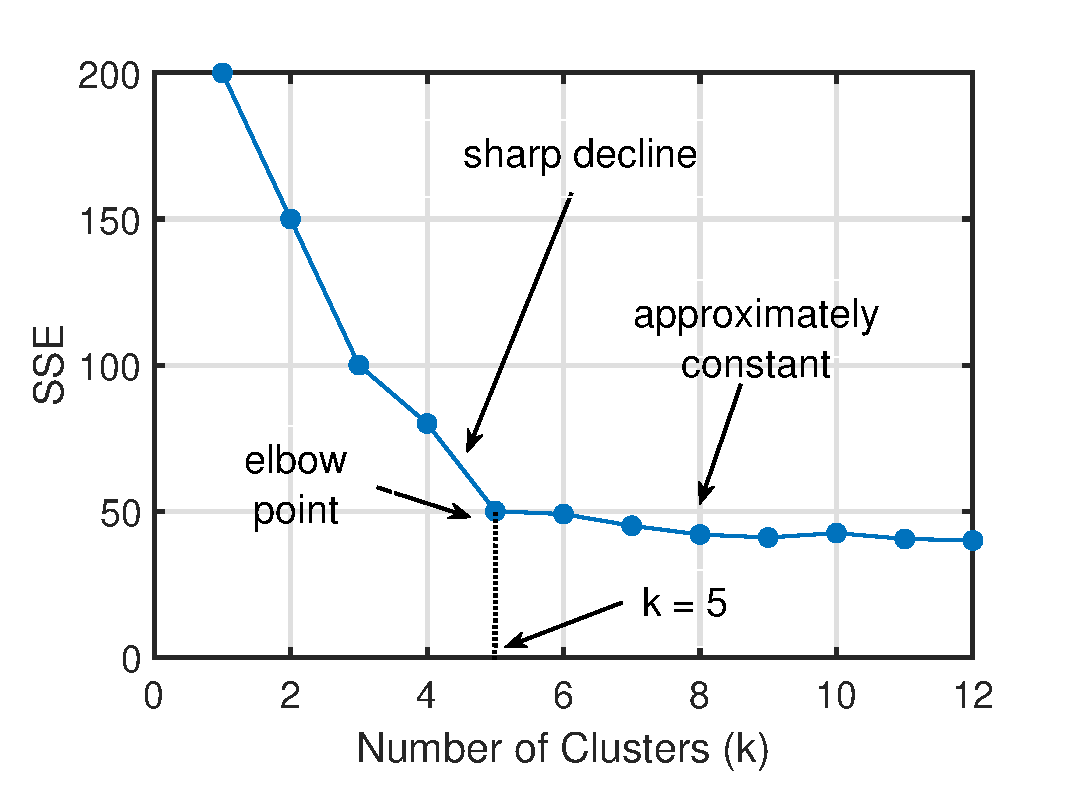
\includegraphics[width=0.45\textwidth]{../minicurso/elbow_ideal.eps}}
        }
        \mbox{
            \subfigure[Silhouette Method.]{
            \label{fig:silhouete-ideal}
            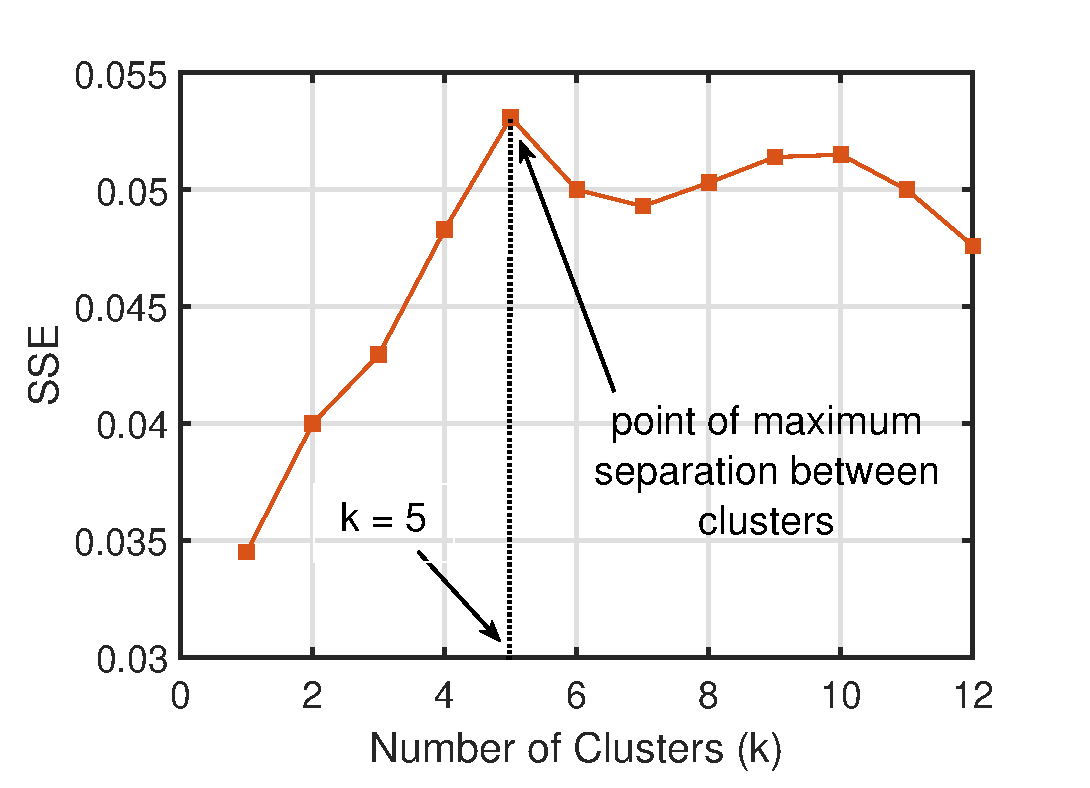
\includegraphics[width=0.45\textwidth]{../minicurso/silhouette_ideal.eps}}
        }
    \end{center}
    \caption{Elbow and Silhouette are complementary methods to determine the optimal number of clusters. Both methods ideally tend to converge to the same k, \textit{e.g.}, $k = 5$ in the example.}
    \label{fig:elbow_silhouette_ideal}
\end{figure}

Both k-means and k-medoids, as well as other algorithms in this classification, are subject to a unique disadvantage: indeterminacy of the appropriate number of clusters $ k $. To circumvent this indeterminacy, the Elbow and the Silhouette methods are used. The goal is to previously analyze the conformity of the data to different amounts of groups and thus obtain a result appropriate to the data. In particular, the Elbow method measures the compaction of clusters by establishing a relationship between the number of clusters and their influence on the total variation of data within the cluster. Graphically, the best $ k $ value is found by identifying the point at which the curve gain decreases dramatically, remaining approximately constant thereafter. Similarly, the Silhouette method measures the quality of a cluster. The ideal number of $ k $ clusters is the one that maximizes the average silhouette over a range of possible values for $ k $~\cite{ketchen1996application, rousseeuw1990finding}. Figure~\ref{fig:elbow_silhouette_ideal} shows a hypothetical usage example of the Elbow and Silhouette methods. In this hypothetical example, it is seen that for the value $ k = 5 $ there is a sharp change in the mean square error (SSE) internal to the clusters observed in the Elbow method and, for $ k = 5 $, there is also a maximum point of the mean error between the clusters in the Silhouette method, indicating a greater separation between clusters.

%Contudo ambos os algoritmos, assim como outros, estão sujeitos à uma desvantagem singular: a indeterminação quanto ao número adequado de grupos $k$. A fim de contornar essa indeterminação, são usados dois métodos, do Cotovelo (\textit{Elbow}) e da Silhueta (\textit{Silhouette}), para analisar previamente a conformidade dos dados a quantidades diferentes de grupos e, assim, obter um resultado adequado aos dados. Em particular, o método do Cotovelo mede a compactação dos agrupamentos estabelecendo uma relação entre o número de agrupamentos e sua influência na variação total dos dados dentro do grupo. Graficamente, o melhor valor de $k$ é encontrado identificando o ponto em que o ganho da curva diminui drasticamente, permanecendo aproximadamente constante depois disso. De forma análoga, o método da Silhueta mede a qualidade de um agrupamento. O número ideal de agrupamentos $k$ é aquele que maximiza a silhueta média em uma faixa de valores possíveis para $k$ \cite{ketchen1996application,rousseeuw1990finding}. A Figura~\ref{fig:elbow_silhouette_ideal} mostra um exemplo hipotético de uso dos métodos do Cotovelo e da Silhueta. Nesse exemplo hipotético, é visto que para o valor $k=5$ há uma mudança brusca no erro médio quadrático (SSE) interno aos agrupamentos no método do Cotovelo e, para $k=5$, também há um ponto máximo do erro médio quadrático entre os agrupamentos no método da Silhueta, indicando maior separação entre agrupamentos.


It should also be noted that there are variations of the \textit{k-means} and \textit{k-medoids} algorithms that consider the degree of relevance of a sample to different groups. In these cases, called \textit{fuzzy k-means} and \textit{fuzzy k-medoids}, the center of the clusters is calculated considering the partial relevance of each sample to the clusters.

%Ressalta-se ainda que há variações dos algoritmos \textit{k-means} e \textit{k-medoids} que consideram graus de pertinência de uma amostra a diversos grupos. Nesses casos, chamados \textit{fuzzy k-means} e \textit{fuzzy k-medoids}, o centro dos agrupamentos são calculados considerando a pertinência parcial de cada amostra aos agrupamentos.

%\subsubsection{Algoritmos Baseados em Densidade}
\subsubsection{Density-Based Algorithms}
\label{subsubsec:densidade}


Density-based clustering algorithms share a close relationship with the nearest neighbor approach. In this sense, a cluster, defined as a dense connected  component, grows in any direction that density leads. This logic of forming clusters is directly related to the main advantage of these algorithms compared to the partitioning algorithms, which is the possibility of discovering clusters with arbitrary shapes, differently from the typically spherical clusters returned by the k-means algorithm, for example.

%Algoritmos de agrupamento baseados em densidade compartilham uma relação próxima com a abordagem do vizinho mais próximo (\textit{nearest neighbour}). Nesse sentido, um agrupamento, definido como um componente denso conectado, cresce em qualquer direção que a densidade o conduza. Essa lógica de formação dos agrupamentos está diretamente relacionada à principal vantagem desses algoritmos em relação ao grupo dos algoritmos de particionamento, a possibilidade de descobrir agrupamentos com formas arbitrárias, diferente dos agrupamentos tipicamente esféricos retornados pelo algoritmo \textit{k-means}, por exemplo.


Among density-based algorithms, the \textbf{Density Based Spatial Clustering of Application with Noise} (DBSCAN) algorithm is the most popular. DBSCAN purpose is to find regions that satisfy an established minimum point density and that are separated by regions of lower density. To this end, the algorithm performs a simple estimate of the minimum density level, defining a limit for the number of neighbors, $ minPts $, within a radius $ \epsilon $. Thus, a sample with more than $ minPts $ neighbors within that radius is considered a central point. Similarly, a sample is considered to be borderline if, within its neighborhood, there are fewer samples than the defined minimum but the sample still belongs to the neighborhood of any central point. Finally, samples that are not reachable by density from any central point, that is, they are neither central nor border points, are labeled as outliers. A disadvantage of this method is its strongly polynomial complexity, which requires $ \Omega \left(n ^ {\frac {4} {3}}\right) $ time to converge, where $ n $ is the size of the dataset~\cite{fahad2014survey, gan2015dbscan, schubert2017dbscan}.

%Dentre os algoritmos baseados em densidade, o algoritmo de \textbf{Clusterização Espacial Baseada em Densidade de Aplicações com Ruído} (\textit{Density Based Spatial Clustering of Application with Noise} -- DBSCAN) é o mais popular. Seu intuito é encontrar regiões que satisfaçam uma densidade de pontos mínima estabelecida e que sejam separadas por regiões de menor densidade. Para isso, o algoritmo realiza uma estimativa simples do nível de densidade mínimo, definindo um limite para o número de vizinhos, $minPts$, dentro de um raio $\epsilon$. Assim, uma amostra com mais de $minPts$ vizinhos dentro desse raio, é considerada um ponto central. Analogamente, uma amostra é considerada como de borda, se dentro de sua vizinhança concentram-se menos amostras que o mínimo definido, porém a amostra ainda pertence à vizinhança de um ponto central qualquer. Por último, amostras que não são alcançáveis por densidade a partir de qualquer ponto central, ou seja, não se configuram nem como pontos centrais nem de borda, são rotulados como \textit{outliers}. Uma desvantagem associada ao seu uso consiste na sua complexidade fortemente polinomial, que requer $\Omega (n^{\frac {4}{3}})$ tempo para convergir, em que $ n $ é o tamanho do conjunto de dados~\cite{fahad2014survey, gan2015dbscan, schubert2017dbscan}.

\subsubsection{Hierarchical Algorithms}
%\subsubsection{Algoritmos Hierárquicos}
\label{subsubsec:hierarquico}

Hierarchical algorithms not only create clusters but consider multi-level logic and calculate a hierarchical representation of the input data. This representation is a particular type of tree, in which the leaf nodes express individual data, and can be constructed using an agglomerative or divisive method. The agglomerative method, also known as the bottom-up approach, begins by considering each sample as a unitary cluster and recursively merging two or more into a new cluster following a chosen link function. Such functions, when associated with distance or similarity metrics, define unique criteria that elect the merged clusters of each iteration. The single link function, for example, establishes the union considering the distance between the samples closest to each cluster. Conversely, the complete link function considers the distance of the most distant samples to each cluster. At the same time, the average link function averages the distances of all samples in one cluster concerning all samples in another cluster. In particular, Ward's criterion employs Euclidean distance in discovering the pair of clusters that minimize the increase in the total internal variance after the union.

%Os algoritmos hierárquicos não apenas criam agrupamentos, mas consideram uma lógica multinível e calculam uma representação hierárquica dos dados de entrada. Esta representação é um tipo particular de árvore, em que os nós-folhas expressam dados individuais, e pode ser construída seguindo um método aglomerativo ou divisivo. O método aglomerativo, conhecido também como abordagem \textit{bottom-up}, começa considerando cada amostra como um agrupamento unitário e mescla recursivamente duas ou mais em um novo agrupamento seguindo uma função de ligação escolhida. Tais funções, quando associados à métricas de distância ou de similaridade, definem critérios únicos que elegem os agrupamentos mesclados de cada iteração. A função de ligação única (\textit{single-linkage}), por exemplo, estabelece a união considerando a distância entre as amostras mais próximos de cada agrupamento. De forma oposta, a função de ligação completa (\textit{complete-linkage}) considera a distância das amostras mais distantes entre si cada agrupamento. Paralelamente, a função de ligação média (\textit{average linkage}) calcula a média das distâncias de todas as amostras de um agrupamento em relação a todas as amostras de outro agrupamento. Em especial, o critério de Ward emprega a distância euclidiana na descoberta do par de agrupamentos que minimizam o aumento na variância total interna após a união.

\begin{figure}[ht]
    \begin{center}
        \mbox{
            \subfigure[Linkage Criteria for the Agglomerative Method]{
            \label{fig:linkage}
            \includegraphics[width=0.45\textwidth]{../minicurso/linkage.png}}
        }
        \mbox{
            \subfigure[Dendrogram]{
            \label{fig:dendrograma}
            \includegraphics[width=0.4\textwidth]{../minicurso/dendograma.png}}
        }
    \end{center}
    \caption{(a) Two-dimensional representation of different connection criteria for the 6 samples already allocated in two clusters. b) Dendrogram resulting from the application of the hierarchical clustering algorithm on samples 1-6. The algorithm employs the agglomerative method using single bond criteria.}
    \label{fig:hiearquico}
\end{figure}

The divisive method, in turn, also known as the top-down approach, starts with a flat structure in which all samples belong to the same cluster, \textit{i.e.}, the same hierarchical level. Therefore, at each iteration, the algorithm divides a parent branch into two smaller subsets, the child branches. The process ends when a stop criterion is reached, often the number $ k $ of clusters. At the end of the algorithm, a clustering dendrogram is created, which is a binary tree hierarchy~\cite {benavent2019fca, icnc-2020-nicollas, fahad2014survey, govender2020application}. A possible hierarchical clustering considering the spatial arrangement between samples 1-6 of Figure~\ref{fig:linkage} is illustrated in Figure~\ref{fig:dendrograma}. Tracing the dotted lines A-D perpendicular to the vertical branches of the dendrogram, it is possible to identify different moments in the clustering process. In $ A $, there are 6 unit clusters, that is, each containing samples. In $ B $, there are 3 clusters: the unit cluster of sample 1, the cluster of samples 2 and 3, and the cluster formed by samples 4, 5, and 6. In $ C $, it is already possible to identify the same pair of groupings depicted in Figure \ref{fig:linkage}. Finally, in $ D $ we verify the presence of a single overpopulated cluster, containing all the initial samples.


%Por outro lado, o método divisivo, e.g. abordagem \textit{top-down}, inicia com uma estrutura plana em que todas as amostras pertencem ao mesmo agrupamento, ou seja, nível hierárquico. Portanto, a cada iteração, o algoritmo divide um ramo-pai em dois subconjuntos menores, os ramos-filhos. O processo termina quando um critério de parada é atingido, frequentemente, o número $ k $ de agrupamentos. No final do algoritmo, é criado um dendrograma de agrupamentos, uma hierarquia de árvore binária~\cite{benavent2019fca, icnc-2020-nicollas, fahad2014survey, govender2020application}. Um possível agrupamento hierárquico considerando a disposição espacial entre as amostras 1-6 da Figura \ref{fig:linkage} é ilustrada na Figura~\ref{fig:dendrograma}. Traçando as retas pontilhadas A-D perpendiculares aos ramos verticais do dendrograma é possível identificar diferentes momentos do processo de agrupamento. Em $A$, nota-se a existência de 6 agrupamentos unitários, ou seja, cada um contendo as amostras. Em $B$, constata-se a existência de 3 agrupamentos: o agrupamento unitário da amostra 1, o agrupamento das amostras 2 e 3, além do agrupamento formado pelas amostras 4, 5 e 6. Em $C$, já é possível identificar o mesmo par de agrupamentos retratados na Figura \ref{fig:linkage}. Por fim, em $D$ verificamos a presença de um único agrupamento superpopuloso, contendo todas as amostras iniciais. 


\subsection{Evaluation Metrics}
%\subsection{Métricas de Avaliação}
\label{subsec:metricasdeavaliação}


Regardless of the supervised or unsupervised algorithm, if there is prior knowledge about data labeled based on a ground truth, it is plausible to clearly identify the number of True Positive (TP), False Positive (FP), True Negatives (TN) and False Negatives (FN). Such classifications make up the calculation of various information retrieval metrics, summarized in Figure~\ref{fig:metricas_roc}, such as the following:

%Independente do algoritmo, supervisionado ou não-supervisionado, caso haja o conhecimento prévio sobre dados rotulados com base em uma verdade básica (\textit{ground truth}), torna-se plausível a clara identificação de quantidade de Verdadeiros Positivos (VP), Falsos Positivos (FP), Verdadeiros Negativos (VN) e Falsos Negativos (FN). Tais classificações compõem o cálculo de várias métricas de recuperação de informação, resumidas na Figura~\ref{fig:metricas_roc}, como:

\begin {itemize}
 \item\textbf{Accuracy} ($ A_c $) is defined by the ratio of the total of correctly classified samples (TP + TN), by the total number of samples (P + N). For unbalanced data sets, a performance assessment based solely on this metric can generate erroneous conclusions;
 
 \item\textbf{Precision} ($ P_r $), given a target class, is the ratio between the number of samples correctly classified for the class in question (TP), by the total set of predictions assigned to that class, \textit{i.e.}, correct and incorrect predictions (TP + FP);
 
 \item\textbf{Sensitivity} ($ S_s $), also known as recall or \textbf{true positive rate}, is defined by the ratio of the number of correctly predicted samples (TP) to a positive class and the total of samples that belong to this class, thus including both correct predictions and those that should have indicated this class (TP + FN). The analog for the negative class is called \textbf {specificity} or \textbf {true negative rate};
 
 \item\textbf {$\pmb{F_{1}} $-Score} relates precision and sensitivity by a harmonic mean expressed by
 
\begin{equation}
 F_{1}\text{-}Score = \frac {2} {\frac {1} {P_ {r}} + \frac {1} {S_ {s}}};
\end{equation}

 Generally, the higher the value of the $ F_ {1} $-Score, the better the classification, reflecting the mutual commitment between precision ($ P_r $) and sensitivity ($ S_s $):
\end{itemize}


%\begin{itemize}
%    \item \textbf{Acurácia} ($A_c$) é definida pela razão do total de amostras classificadas corretamente (VP + VN), pelo número total de amostras (P+N). Para conjunto de dados não-balanceados, uma avaliação de desempenho baseada exclusivamente nesta métrica pode gerar conclusões erradas;
%    \item \textbf{Precisão} ($P_r$) é a razão entre, dada uma classe alvo, a quantidade de amostras corretamente classificadas para a classe em questão (VP), pelo conjunto total de predições atribuídas a essa classe, isto é, corretas e incorretas (VP + FP);
%    \item \textbf{Sensibilidade} ($S_s$) também conhecida como revocação (\textit{recall}) ou \textbf{taxa de verdadeiros positivos} é definida pela razão entre a quantidade de amostras corretamente preditas (VP) para um classe positiva e o total de amostras que pertencem a esta classe, incluindo assim tanto predições corretas quanto as que deveriam ter indicado esta classe (VP + FN). O análogo para a classe negativa é chamado de \textbf{especificidade} ou \textbf{taxa de verdadeiros negativos};
%    \item \textbf{Medida-$F_{1}$} (\textit{$F_{1}$-Score}) relaciona a precisão e a sensibilidade por uma média harmônica expressa por 
%\begin{equation}
%    Medida-F_{1} = \frac{2}{\frac{1}{P_{r}}+\frac{1}{S_{s}}};
%\end{equation}
%    Geralmente, quando maior o valor da medida-$F_{1}$, melhor a classificação sendo um reflexo do compromisso mútuo entre a precisão ($P_r$) a sensibilidade ($S_s$): 
%\end{itemize}

\begin{itemize}
    \item \textbf{Area under the ROC Curve} (AUC) is measured using the Receiver Operation Characteristic (ROC) curve, shown in Figure~\ref{fig:_ideal}, which represents the ratio between the true positive rate (TPR) and the false positive rate (FPR), for several cutoff thresholds. This curve graphically describes the performance of a classification model. Briefly, the larger the area under the curve (closer to the unit value), the better the performance of the model, regardless of the cutoff point of the probability of the sample belonging to each class.
    %é medida através da curva Característica de Operação do Receptor (ROC), mostrada na Figura~\ref{fig:_ideal}, uma representação da razão entre a taxa de verdadeiros positivos (TPR) e a taxa de falsos positivos (FPR), para vários limiares de corte. Essa curva descreve graficamente o desempenho de um modelo de classificação. Sucintamente, quanto maior a área abaixo da curva (mais próxima ao valor unitário), melhor o desempenho do modelo, independentemente do ponto de corte da probabilidade de pertencimento de à classe de cada amostra. 
\end{itemize}

\begin{figure}[ht]
    \begin{center}
        \mbox{
            \subfigure[ROC Curve]{
            \label{fig:_ideal}
            \includegraphics[width=0.35\textwidth]{../minicurso/roc_ideal.png}}
        }
        \mbox{
            \subfigure[Information Retrieving Metrics]{
            \label{fig:metricas}
            \includegraphics[width=0.40\textwidth]{../minicurso/metricas.png}}
        }
    \end{center}
    \caption{(a) ROC curve of classifiers and comparison of the Area Under the ROC Curve (AUC). (b) Accuracy, precision and sensitivity metrics in a binary classification problem.}
    \label{fig:metricas_roc}
\end{figure}


\section{Research Initiatives}
\label{sec:research}

Several research activities exist and seek to characterize and mitigate the challenges caused by fake news. Lazer \textit {et al.} formalize an initial definition of fake news and discuss the historical background of fake news, starting with defamation in the First World War until the impact of fake news during the United States presidential election in 2016~\cite{lazer2018science}. Grinberg \textit{et al.} delve into the impact of fake news during the 2016 elections, analyzing messages from the  \textit{Twitter} social network~\cite{grinberg2019fake}. The authors collected tweets sent by 16,442 active accounts during the 2016 electoral season, from August 1 to December 6, 2016. The results show that groups of older users, who are between 60 and 80 years old, with right-wing or extreme right political affinity  are more likely to distribute and share fake political news. The recent 2019 Coronavirus Infectious Disease pandemic (COVID-19) is also an event in which a large amount of fake news is disseminated. Recent studies show the correlation between social media usage and misinformation during the pandemic~\cite{pennycook2020fighting, van2020using}.
%Diversas atividades de pesquisa estão ativas e buscam caracterizar e mitigar os desafios causados pelas notícias falsas.
%Uma definição inicial sobre as notícias falsas é feita por Lazer \textit{et al.}. No artigo, é abordada a historia das notícias falsas começando pela difamação na Primeira Guerra Mundial até o impacto das notícias falsas durante a eleição presidencial dos Estados Unidos em 2016~\cite{lazer2018science}. Grinberg \textit{et al.} aprofundam no impacto das notícias falsas durante as eleições de 2016, analisando as mensagens da rede social \textit{Twitter}~\cite{grinberg2019fake}. Os autores coletaram \textit{tweets} enviados por 16.442 contas ativas durante a temporada eleitoral de 2016, de 1º de agosto até 6 de dezembro de 2016. Os resultados mostram que os grupos de maior idade, entre 60 e 80 anos, com afinidade politica de direita ou extrema direita são mais propensos à distribuição e ao compartilhamento de notícias políticas falsas. A recente pandemia da Doença Infecciosa por Corona Vírus de 2019 (COVID-19) também é um evento no qual foram disseminadas grande quantidade de notícias falsas. Estudos recentes mostram a correlação entre o uso de mídia social e a desinformação durante a pandemia~\cite{pennycook2020fighting, van2020using}.  


The detection of fake news is studied from several perspectives, such as Machine Learning, Data Mining, and Natural Language Processing. The Bag-of-Words and the frequencies of categories are used to train classifiers such as Support Vector Machines (SVM) and naive Bayesian models \cite{poddar2019comparison}. Since the mathematical model is trained from known examples of the two categories, false and legitimate news, it is possible to predict future instances based on numerical clustering and distances. The use of different clustering methods and distance functions is one of the SVM algorithm bases. The naive Bayesian algorithm, in turn, makes classifications based on accumulated evidence of the correlation between a given variable, such as syntax, and the other variables present in the model.
%A detecção de notícias falsas é estudada sob várias perspectivas como Aprendizado de Máquina, Mineração de Dados e Processamento de Linguagem Natural. O Saco-de-Palavras e as frequências de categorias são utilizadas para  o treinamento de classificadores como as Máquinas de Vetores Suportes (\textit{Support Vector Machines } - SVM) e modelos bayesianos ingênuos~\cite{poddar2019comparison}. Uma vez que o modelo matemático é treinado a partir de exemplos conhecidos das duas categorias, notícia falsa ou não, é possível prever instâncias futuras com base em agrupamento numérico e distâncias. O uso de diferentes métodos de agrupamento e funções de distância entre os pontos de dados é uma das bases do algoritmo do SVM. Por outro lado, o algoritmo bayesiano ingênuo faz classificações com base em evidências acumuladas da correlação entre uma determinada variável, como a sintaxe, e as outras variáveis presentes no modelo.

Shu \textit {et al.} review the detection of fake news on social media from a data mining perspective, including characterization of fake news on psychology and social theories, existing algorithms, evaluation metrics, and representative datasets~\cite{shu2017fake}. Fake News Tracker is a solution for data collection, interactive visualization, and analytical modeling for detecting fake news. The solution uses Natural Language Processing techniques~\cite{shu2019fakenewstracker}.
%Shu \textit{et al.} fazem uma revisão da detecção de notícias falsas nas mídias sociais de uma perspectiva de mineração de dados, incluindo caracterização de notícias falsas sobre psicologia e teorias sociais, algoritmos existentes, métricas de avaliação e conjuntos de dados representativos~\cite{shu2017fake}. \textit{Fake News Tracker} é uma solução para coleta de dados, visualização interativa e modelagem analítica para detecção de notícias falsas. A solução utiliza técnicas de Processamento de Linguagem Natural~\cite{shu2019fakenewstracker}. 
%
Other papers present techniques and challenges related to the detection of fake news. Zhou and Zafarani identify and detail fundamental theories related to different disciplines for detecting fake news~\cite{zhou2018fake}. Sharma \textit{et al.} discuss existing methods and techniques that apply to the identification and mitigation of fake news, focusing on the significant advances in each method and their advantages and limitations~\cite{sharma2019combating}. Bondielli and Marcelloni survey the literature on the different approaches for automatically detecting fake news and rumors~\cite{BONDIELLI201938}. The authors highlight several approaches taken to collect fake news and rumor data.
%Alguns trabalhos apresentam técnicas e desafios sobre a detecção de notícias falsas. Zhou e Zafarani identificam e detalham as teorias fundamentais relacionadas em diferentes disciplinas para a detecção de notícias falsas~\cite{zhou2018fake}. Sharma \textit{et al.} discutem os métodos e técnicas existentes aplicáveis à identificação e à mitigação de notícias falsas, com foco nos avanços significativos em cada método e suas vantagens e limitações~\cite{sharma2019combating}. Bondielli e Marcelloni fazem um levantamento da literatura sobre as diferentes abordagens para a detecção automática de notícias falsas e rumores~\cite{BONDIELLI201938}. Os autores destacam várias abordagens adotadas para coletar dados de notícias falsas e rumores. 

Oshikawa \textit {et al.} presents a comparison of the methods used to detect fake news using Natural Language Processing (NLP)~\cite{oshikawa2018survey}. Similarly, Sharma \textit{et al.} analyze the literature review on NLP applied to fake news, highlighting the comparison between different machine learning techniques, deep learning, and other techniques~\cite{sharma2019combating}. Deepak and Chitturi compare different types of neural networks in detecting fake news~\cite{deepak-lstm}. Feng \textit{et al.} propose a two-level convolutional neural network with a user response generator, in which the neural network captures semantic information from the text, representing it at  phrase- and word-level. The user-response generator learns a model of the user's response to the news text~\cite{fengAndSharma}.
%Oshikawa \textit{et al.} apresentam uma comparação dos métodos usados na detecção de notícias falsas usando Processamento de Linguagem Natural (PLN)~\cite{oshikawa2018survey}. De forma semelhante, Sharma \textit{et al.} analisam a revisão da literatura sobre PLN aplicado em notícias falsas, ressaltando a comparação entre as diferentes técnicas de aprendizado de máquina, aprendizado profundo e outras técnicas~\cite{sharma2019combating}. Deepak and Chitturi compararam diferentes tipos de redes neuronais na detecção de notícias falsas~\cite{deepak-lstm}. Feng \textit{et al.} propõem uma rede neural convolucional de dois níveis com gerador de resposta do usuário, em que a rede neural captura informações semânticas do texto, representando-as no nível de frase e de palavra, e o gerador de resposta de usuário aprende um modelo da resposta do usuário ao texto da notícia~\cite{fengAndSharma}. 


% definition
% https://www.tandfonline.com/doi/full/10.1080/21670811.2017.1360143?scroll=top&needAccess=true

% surveys

% https://www.pnas.org/content/pnas/116/16/7662.full.pdf
% https://arxiv.org/pdf/1812.00315.pdf
% https://dl.acm.org/doi/pdf/10.1145/3289600.3291382?casa_token=kqo_C2LbUlEAAAAA:E4Nq2-EEpAmvSdtIbxt6ZZbXRlhd86f_sqiohFtWo09Bzvz3tu5d_676sVrHfrFaI8Ntu8i13ACE
% https://dl.acm.org/doi/pdf/10.1145/3377330.3377334?casa_token=lNBcZUFGRuIAAAAA:mVMmVItRoPLuxK1DqxP8tiRhXyqVcrJfjuMvVztT7NyvuulMiSFmYVJbhCOilfwTb2CdQ9MjY9bF
% http://pike.psu.edu/publications/abs19.pdf
% https://philpapers.org/archive/PEPWNA.pdf
% https://onlinelibrary.wiley.com/doi/abs/10.1111/soc4.12724
% http://www.andrewtlittle.com/papers/little_fakenews_cp.pdf
% https://www.sciencedirect.com/science/article/abs/pii/S016792362030035X
% http://sbp-brims.org/2018/proceedings/papers/challenge_papers/SBP-BRiMS_2018_paper_116.pdf
% https://commons.emich.edu/cgi/viewcontent.cgi?article=1322&context=loexquarterly
% https://dspace.lib.uom.gr/bitstream/2159/23448/4/RaptiMatinaMsc2019.pdf
% https://www.sciencedirect.com/science/article/pii/S2352250X20300439
% https://www.researchgate.net/profile/Xinyi_Zhou26/publication/342762209_A_Survey_of_Fake_News_Fundamental_Theories_Detection_Methods_and_Opportunities/links/5f1644f9a6fdcc3ed71b23cd/A-Survey-of-Fake-News-Fundamental-Theories-Detection-Methods-and-Opportunities.pdf

% covid 
% https://www.researchgate.net/profile/Beatriz_Villarejo/publication/340658737_COVID-19_infodemic_More_retweets_for_science-based_information_on_coronavirus_than_for_false_information/links/5e99749c299bf13079a203b8/COVID-19-infodemic-More-retweets-for-science-based-information-on-coronavirus-than-for-false-information.pdf
% https://www.ncbi.nlm.nih.gov/pmc/articles/PMC7202120/
% https://arxiv.org/pdf/2007.09682
% https://www.ncbi.nlm.nih.gov/pmc/articles/PMC7390799/


% us election
% https://dl.acm.org/doi/pdf/10.1145/3308558.3313721?casa_token=jLo5nde502UAAAAA:S6SpC1qIVkMjWIJdLFFd8Ux5sTZsqfeWOaj6XP9yhdSY0nkr0qDIhOc1vmzpVXivHijj85dmYYs5
% https://www.nber.org/papers/w23089.pdf
% http://www.ask-force.org/web/Fundamentalists/Guess-Selective-Exposure-to-Misinformation-Evidence-Presidential-Campaign-2018.pdf

% data mining
% http://www.vldb.org/pvldb/vol12/p1990-lakshmanan.pdf


% model
% https://apps.dtic.mil/dtic/tr/fulltext/u2/1061567.pdf
% https://dl.acm.org/doi/pdf/10.1145/3377478

% portuguese and detection
% https://www.sciencedirect.com/science/article/abs/pii/S0957417420300257
% https://arxiv.org/pdf/1705.00648.pdf
% https://asistdl.onlinelibrary.wiley.com/doi/pdf/10.1002/pra2.2015.145052010083
% https://asistdl.onlinelibrary.wiley.com/doi/pdf/10.1002/pra2.2015.145052010082

% facebook
% https://advances.sciencemag.org/content/5/1/eaau4586.full

% social bots
% https://www.andyblackassociates.co.uk/wp-content/uploads/2015/06/fakenewsbots.pdf

% NLP
% https://sci-hub.st/https://ieeexplore.ieee.org/abstract/document/8665593
% https://www.sciencedirect.com/science/article/abs/pii/S095741741930661X

% machine learning
% https://www.researchgate.net/profile/Marina_Ibrishimova/publication/335191041_A_Machine_Learning_Approach_to_Fake_News_Detection_Using_Knowledge_Verification_and_Natural_Language_Processing/links/5dd0b7db299bf1b74b48ac28/A-Machine-Learning-Approach-to-Fake-News-Detection-Using-Knowledge-Verification-and-Natural-Language-Processing.pdf

%\section{Desafios e Oportunidades de Pesquisa}
\section{Research Challenges and Opportunities}
\label{sec:desafios}

Research into identifying, detecting, and mitigating the spread of fake news is still under development. Nevertheless, it is already possible to identify the main challenges in combating fake news, which are listed following~\cite{sharma2019combating}.

%Embora as pesquisas na identificação, detecção e mitigação da propagação de notícias falsas estejam em pelo desenvolvimento, alguns dos principais desafios no combate às notícias falsas são listados a seguir~\cite{sharma2019combating}.

\begin{itemize}

\item{\bf Great interests and the plurality of actors involved.} Due to the volume that the spread of fake news reaches on social networks in a short period, fake news pose a threat to traditional sources of information, such as traditional press. The spread of fake news occurs as a distributed event, and involves multiple entities and technological platforms. Thus, there is an increasing difficulty in studying and designing computational, technological, and business strategies to combat fake news without compromising speed and collaborative access to high-quality information.

%\item {\bf Grandes interesses e a pluralidade de atores envolvidos.} Devido ao volume que a propagação de notícias falsas atinge em redes sociais em um período curto, as notícias falsas representam uma ameaça às fontes tradicionais de informações, como a impressa tradicional. O espalhamento de notícias falsas ocorre como um evento distribuído e, então, envolve múltiplas entidades e plataformas tecnológicas. Assim, há uma crescente dificuldade de estudar e projetar estratégias computacionais, tecnológicas e de negócios de combate às notícias falsas sem que haja o comprometimento da rapidez e do acesso colaborativo a informações de alta qualidade.

\item{\bf Opponent's malicious intent.} The fake news content is designed to make it difficult for humans to identify the fake news, exploiting our cognitive skills, emotions, and ideological prejudices. Moreover, it is challenging for computational methods to detect fake news, as the way fake news is presented is similar to true news, and sometimes fake news uses artifices to make it difficult to identify the source or falsify the real source of the news.

%\item {\bf Intenção maliciosa do adversário.} O conteúdo das notícias falsas é projetado para dificultar a identificação por humanos das notícias falsas, explorando suas habilidades cognitivas, emoções e preconceitos ideológicos. Além disso, é desafiador para métodos computacionais detectar notícias falsas, pois a forma como as notícias falsas são apresentadas é semelhante à de notícias verídicas e, por vezes, as notícias falsas usam artifícios para dificultar a identificação da fonte ou falsificam a verdadeira fonte da notícia.


\item{\bf Susceptibility and lack of public awareness.} The user of social networks is subject to a large amount of information from dubious origins, from information with a humorous nature, such as satires, to information intended to deceive the consumer of the information posing as legitimate news. However, the user of social networks is not able to differentiate fake news from legitimate news just by content. The user does not have information about the credibility of the source or patterns of spreading of the news on the network. Thus, to increase public awareness, several articles and advertising campaigns are run to provide tips on how to differentiate between false and legitimate news. For example, the University of Portland in the United States provides a guide for identifying misinformation (fake news)\footnote{Available at https://guides.library.pdx.edu/c.php?g=625347\&p=4359724}.

%\item {\bf Suscetibilidade e falta de conscientização do público.} O usuário de redes sociais está sujeito a uma grande quantidade de informações de origens duvidosas, desde informações com cunho humorístico, como sátiras, até informações com o intuito de enganar o consumidor de informações se passando por notícias verídicas. Contudo, o usuário de redes sociais não é capaz de diferenciar uma notícia falsa de uma verídica apenas pelo conteúdo. O usuário não dispõe de informações sobre a credibilidade da fonte ou padrões de propagação da notícia na rede. Assim, para aumentar a conscientização pública, vários artigos e campanhas publicitárias são veiculados para fornecerem dicas sobre como diferenciar notícias verídicas de falsas. Por exemplo, a Universidade de Portland, nos Estados Unidos, disponibiliza um guia para a identificação de desinformação (notícias falsas)\footnote{Disponível em https://guides.library.pdx.edu/c.php?g=625347\&p=4359724.}. 

\item {\bf Propagation dynamics.} The spread of fake news on social media complicates detection and mitigation, as fake information can easily reach and affect large numbers of users in a short time. The information is transmitted quickly and easily, even when its veracity is doubtful~\cite{friggeri2014}. Verification of veracity must be carried out in an agile way, but it must also consider the patterns of propagation of information throughout the network~\cite{meel2020}.

%\item {\bf Dinâmica de propagação.} A propagação de notícias falsas em mídia social complica a detecção e a mitigação, pois as informações falsas podem facilmente alcançar e afetar um grande número de usuários em pouco tempo. A informação é transmitida de maneira rápida e fácil, mesmo quando sua veracidade é duvidosa~\cite{friggeri2014}. A verificação da veracidade deve ser realizada de forma ágil, mas também deve considerar os padrões de propagação da informação ao longo da rede~\cite{meel2020}.

\item{\bf Constant changes in the characteristics of fake news.} Developments in the automated identification of fake news also drive the adaptation of the generation of new disinformation content to avoid being classified as such. The detection of fake news based on writing style, differentiating false and legitimate news by an analysis based on Natural Language Processing, is one of the main used alternatives due to the unsolved challenges in automatic fact verification from pre-defined knowledge bases. Thus, current approaches to identify fake news based on the content focus on extracting facts directly from the news content and subsequent verification of the facts against knowledge bases~\cite{ciot-nicollas-2020}.

%\item {\bf Mudanças constante das características das notícias falsas.} Os desenvolvimentos na identificação automatizada de notícias falsas também impulsionam a adaptação da geração de novos conteúdos de desinformação para evitarem de serem classificados como tal. A detecção de notícias falsas baseada em estilo de escrita, diferenciando notícias falsas e verdadeiras por uma análise baseada no processamento de linguagem natural, é uma das principais alternativas usadas devido aos desafios não resolvidos na automatização da verificação de fatos a partir de bases de conhecimento pré-definidas. Assim, abordagens atuais de identificação de notícias falsas baseadas no conteúdo focam na extração de fatos diretamente do conteúdo da notícia e a posterior verificação dos fatos contra bases de conhecimento~\cite{ciot-nicollas-2020}.


\item{\bf Attacks on natural language learning.} Zhou {\it et al.} argue that the use of Natural Language Processing to identify fake news is vulnerable to attacks on the machine learning itself~\cite{zhou-arxiv}. Zhou {\it et al.} identify three attacks: the distortion of facts, the exchange between subject and object, and the confusion of causes. The distortion is, in fact, to exaggerate or modify some words. Textual elements, such as characters and time, can be distorted to lead to a false interpretation. The exchange between subject and object aims to confuse the reader between those who practice and those who suffer the reported action. The attack of confusion of cause consists of creating non-existent causal relations between two independent events or cutting parts of a story, leaving only the parts that the attacker wishes to present to the reader~\cite{zhou-arxiv}.

%\item {\bf Ataques ao aprendizado por linguagem natural.} Zhou {\it et al.} argumentam que o uso de processamento de linguagem natural para a identificação de notícias falsas é vulnerável a ataques ao aprendizado de máquina em si~\cite{zhou-arxiv}. Zhou {\it et al.} identificam três ataques: a distorção de fatos, a troca entre sujeito e objeto; e a confusão de causas. A distorção de fato consiste em exagerar ou modificar algumas palavras. Elementos textuais, como personagens e tempo, podem ser distorcidos para levar a uma interpretação falsa. A troca entre sujeito e objeto tem como objetivo confundir o leitor entre quem pratica e quem sofre a ação relatada. O ataque de confusão de causa consiste em criar relações causais inexistentes entre dois eventos independentes ou cortar partes de uma história, deixando apenas as partes que o atacante deseja apresentar para o leitor~\cite{zhou-arxiv}.

\end{itemize}

Research opportunities to identify and mitigate fake news focus on rapid or real-time detection of the source, controlling the spread of false information and reducing the impact of fake news on society. Dataset collected in real-time, automatic detection of rumors, and location of the source are challenging research questions~\cite{meel2020}. The main opportunities for research and development of solutions to combat fake news are highlighted following.

%As oportunidades de pesquisa na identificação e mitigação de notícias falsas focam na detecção rápida ou em tempo real da fonte, no controle da propagação das informações falsas e na redução do impacto das notícias falsas na sociedade. Conjuntos de dados coletados em tempo real, detecção automática de rumores e localização da fonte original são questões de pesquisa desafiadoras~\cite{meel2020}. A seguir destacam-se as principais oportunidades de pesquisa e desenvolvimento de soluções para o combate às notícias falsas.

\begin{itemize}
    \item {\bf Extracting the most significant features.} Determining the most effective features for detecting fake news from multiple data sources is an open research opportunity. Fundamentally, there are two main data sources: news content and social context~\cite{shu2017fake}. From a news content perspective, techniques based on Natural Language Processing and feature extraction can be used to extract information from the text. Embedding techniques, such as word embedding and deep neural networks are the focus of current researches for the extraction of textual characteristics, and they have the potential to learn better representations for the data. Visual characteristics extracted from the images are also important indicators of fake news. The use of deep neural networks is an opportunity for research in the extraction of visual characteristics for the detection of fake news~\cite{sharma2019combating, meel2020}.
    
    %\item {\bf Extração de características mais significativas.} Determinar as características mais eficazes para detectar notícias falsas de múltiplas fontes de dados é uma oportunidade de pesquisa em aberto. Fundamentalmente, existem duas fontes de dados principais: o conteúdo das notícias e contexto social~\cite{shu2017fake}. Da perspectiva de conteúdo de notícias, técnicas baseadas em processamento de linguagem natural e extração de características podem ser usadas para extrair informações do texto. Técnicas de incorporação, como incorporação de palavras (\textit{word embedding}) e redes neurais profundas são foco de pesquisas atuais para a extração de características textuais e têm o potencial para aprender melhores representações para os dados. Características visuais extraídas das imagens também são indicadores importantes para notícias falsas. O uso de redes neurais profundas é uma oportunidade de pesquisa na extração de características visuais para a detecção de notícias falsas~\cite{sharma2019combating,meel2020}.

    \item{\bf Detection on different platforms and different domains.} Since that users use different social networks, fake news, and rumors spread across different platforms, making it difficult to locate the source of the news or rumor. Tracing the source of false information between different social media platforms is a research opportunity. Therefore, several aspects of the information must be considered. However, most of the existing approach focuses only on one way of detecting false information: analysis of content, propagation, style, among others. The analysis must then consider different attribute domains, such as topics, web sites, images, and URLs~\cite{meel2020}.
    
    %\item {\bf Detecção em diferentes plataformas e diferentes domínios.}  Devido ao fato dos usuários utilizarem diferentes redes sociais, as notícias falsas e boatos se espalham nas diferentes plataformas, dificultando a localização da origem da notícia ou do boato. O rastreamento da origem da informação falsa entre plataformas distintas de redes sociais é uma oportunidade de pesquisa. Para tanto, devem ser considerados diversos aspectos da informação. Contudo, a maior parte da abordagem existente se concentra apenas em uma das formas de detecção da informação falsa: análise de conteúdo, da propagação, do estilo, entre outras. A análise deve considerar, então, diferentes domínios de atributos, como tópicos, sítios \textit{web}, imagens e URLs~\cite{meel2020}.

    \item{\bf Identification of echo chambers and bridges between chambers.} Social media tends to form echo chambers in communities where users have similar views and ideologies. Users have their views reinforced and are not aware of the opposite beliefs. Therefore, research is needed to identify conflicting echo chambers and connect chambers with opposite positions so that users are faced with different points of view. This bridging also helps in discovering the truth, making users think carefully and rationally in multiple dimensions~\cite{meel2020}.

    %\item {\bf Identificação de câmaras de eco e ponte entre as câmaras.}  A mídia social tende a formar câmaras de eco em comunidades em que usuário têm visões e ideologias semelhantes. Os usuários têm suas visões reforçadas e não estão cientes das crenças opostas. Portanto, pesquisas são necessárias para identificar câmaras de eco conflitantes e ligar as câmaras com posições opostas para que os usuários sejam confrontados com visões distintas. Isso também ajuda na descoberta da verdade, fazendo os usuários pensarem criteriosamente e racionalmente em múltiplas dimensões~\cite{meel2020}.
    
    \item {\bf Development of machine learning models.} There is a need for research in the development of real-time learning models, such as incremental learning and federated learning, capable of learning from manually verified articles and providing real-time detection of new articles with fraudulent information. Another important point is the development of unsupervised models in which the algorithms learn from real data and, then, articles that escape the behavior of real data are classified as false. There is still a dearth of specific datasets for fake news. The lack of publicly available large-scale datasets implies a lack of tests (benchmarks) for comparing the performance of different algorithms~\cite{meel2020}.
    
    %\item {\bf Desenvolvimento de modelos de aprendizado de máquina.} Há a necessidade de pesquisa no desenvolvimento de modelos de aprendizado em tempo real, tais como aprendizado incremental e aprendizado federado, capazes de aprender com artigos verificados manualmente e fornecer detecção em tempo real de novos artigos com informações fraudulentas. Outro ponto importante é o desenvolvimento de modelos não-supervisionados em que os algoritmos aprendem com dados reais e, então, artigos que fogem do comportamento de dados reais são classificados como falsos. Há ainda uma escassez de conjuntos de dados específicos para notícias falsas. A falta de conjuntos de dados de larga escala publicamente disponíveis implica a carência de testes (\textit{benchmarks}) para a comparação de desempenho entre algoritmos diferentes~\cite{meel2020}.

    \item {\bf Development of data structures capable of handling complex and dynamic network structures.} The complexity and dynamics of social network relationship structures make the task of identifying and tracking posts more complicated. Thus, there is a need to develop complex data structures that reflect the dynamics of relationships in social networks to allow the extraction of knowledge about the spread of false information throughout the network~\cite{meel2020}.

    %\item {\bf Desenvolvimento de estruturas de dados capazes de lidar com a estrutura de rede complexa e dinâmica.}  A complexidade e a dinamicidade das estruturas de relacionamento em redes sociais tornam a tarefa de identificação e rastreamento de publicações mais complicadas. Assim, há a necessidade de pesquisa para o desenvolvimento de estruturas de dados complexas que reflitam a dinamicidade das relações em redes sociais para permitir a extração de conhecimento acerca da propagação de informações falsas na rede~\cite{meel2020}.

\end{itemize}


\section{Conclusion}
\label{sec:conclusion}

In this paper, definitions, characteristics and the process of disseminating fake news were presented. We also discussed the traditional methods for detecting fake news. The most recent reference databases used in this area of research were compared. The literature shows that Natural Language Processing (NLP) has been used to detect fake news. We discussed how NLP can be used to evaluate information from  social networks and a comparison with the different machine learning methods was also presented. % This short course tries to provide a holistic view of the information pollution ecosystem in terms of taxonomy of fraudulent content, life cycle of a complete ecosystem, different digital media platforms, main driving forces behind the spread of disinformation and different platforms of credibility analysis.
In addition, open questions and challenges are also highlighted to explore potential research opportunities. This work is useful for researchers to understand the different components of online digital communication from a social and technical perspective. Dissemination of fake news on multiple multilingual platforms, complex and dynamic network structure, large volumes of real-time unlabeled data and early detection of rumors are some challenging problems that are yet to be solved and need further research. %Finally, the practical activity developed shows the feasibility in detecting false news.
Improving the reliability and future of the information ecosystem online is a joint responsibility of the scientific community, digital policy makers, management and society.

%Nesse minicurso foram apresentadas as definições, características e o processo de disseminação de notícias falsas. Em seguida, foram discutidos os métodos tradicionais para a detecção de notícias falsas. Foram comparados os conjuntos de dados de referência mais recentes. Com base em trabalhos da literatura, foi proposto a utilização do Processamento de Linguagem Natural (PLN) na de detecção de notícias falsas. Foram mostrados como o PLN pode ser usado sobre redes sociais e uma comparação com os diferentes métodos de aprendizado de máquina utilizados.
%Este minicurso tenta fornecer uma visão holística do ecossistema de poluição da informação em termos de taxonomia de conteúdos fraudulentos, ciclo de vida de um ecossistema completo, diferentes plataformas de comunicação social digital, principais forças motrizes por trás da disseminação da desinformação e diferentes plataformas de análise de credibilidade. 
%Além disso, questões em aberto e desafios também são destacados para explorar as oportunidades de pesquisa em potencial. Esse trabalho é útil para os pesquisadores compreendam os diferentes componentes da comunicação digital \textit{online} de uma perspectiva social e técnica. Divulgação de notícias falsas em várias plataformas multilíngues, estrutura de rede complexa e dinâmica, grandes volumes de dados em tempo real não rotulados e detecção precoce de boatos são alguns problemas desafiadores que ainda não foram resolvidos e necessitam mais pesquisas. 
%Finalmente, a atividade prática desenvolvida mostrar a viabilidade na detecção de notícias falsas.
%Melhorar a confiabilidade e o futuro do ecossistema de informações \textit{online} é uma responsabilidade conjunta da comunidade científica, formuladores de políticas digitais, administração e da sociedade em geral.


\bibliographystyle{IEEEtran}
\bibliography{biblio}


\begin{IEEEbiography}[{\includegraphics[width=1in,height=1.25in,clip,keepaspectratio]{photos/nicollas.png}}]{Nicollas Rodrigues de Oliveira} is currently a PhD student in Telecommunications Engineering at Universidade Federal Fluminense. He got his master's degree in Telecommunications Engineering from Universidade Federal Fluminense (UFF) in 2020, and he graduated in Telecommunications Engineering at the same university in 2018. Between 2016 and 2018, he was a volunteer student, and later, he was a scholarship holder for a scientific initiation project. 
\end{IEEEbiography}

\begin{IEEEbiography}[{\includegraphics[width=1in,height=1.25in,clip,keepaspectratio]{photos/martin.jpg}}]{Martin Andreoni Lopez} is a researcher of the Secure Systems Research Centre (SSRC) at Technology Innovation Institute (TII), United Arab Emirates. He graduated as an Electronics Engineer from \textit{Universidad Nacional de San Juan} (UNSJ), Argentina, in 2011. He got his Master's degree in Electrical Engineering from the \textit{Universidade Federal do Rio de Janeiro} (COPPE / UFRJ) in 2014. He got his PhD degree both from the \textit{Universidade Federal do Rio de Janeiro} (COPPE / UFRJ) in the Teleinformatics and Automation Group (GTA), and from \textit {Sorbonne Université} in the Phare team of the \textit {Laboratoire d'Informatique de Paris VI} (LIP6), France. He has several publications and patents in security, virtualization, network traffic analysis, and Big Data analytics. 
\end{IEEEbiography}

\begin{IEEEbiography}[{\includegraphics[width=1in,height=1.25in,clip,keepaspectratio]{photos/dianne.jpg}}]{Dianne Scherly Varela de Medeiros} is a professor at the Universidade Federal Fluminense (UFF). Dianne received her Master’s degree on Telecommunications Engineering from UFF in 2013, and her D.Sc. degree on Electric Engineering from the Universidade Federal do Rio de Janeiro in 2017. Between 2015 and 2016, she had a sandwich scholarship to work on her Ph.D. Thesis on the LIP6 (Laboratoire d’Informatique de Paris 6) at Sorbonne Université, Paris, France.
\end{IEEEbiography}

\begin{IEEEbiography}[{\includegraphics[width=1in,height=1.25in,clip,keepaspectratio]{photos/diogo.jpg}}]{Diogo Menezes Ferrazani Mattos} is a professor at the Universidade Federal Fluminense (Niterói, Brazil). He received his degrees of D.Sc. and M.Sc. in Electrical Engineering from Universidade Federal do Rio de Janeiro, Rio de Janeiro, Brazil, in 2017 and 2012. Between 2015 and 2016, he had a sandwich scholarship to work on his Ph.D. Thesis on the LIP6 (Laboratoire d’Informatique de Paris 6) at Université Pierre et Marie Curie, Paris, France. He received a Computer and Information Engineer degree from Universidade Federal do Rio de Janeiro, in 2010, awarded with Magna Cum Laude.
\end{IEEEbiography}
\vfill
\EOD

\end{document}
